%\newif\iffull
%\fulltrue

%\iffull
%\documentclass{article}
%\else
%\documentclass{llncs}
%\fi

%\usepackage{epsf}

%% macros.tex
%
% Macros for this paper. (Include build/headers.tex, then this.)
%\usepackage{times}
%\usepackage[dvipdf]{graphicx}
\usepackage{pifont} % \ding{109}
\usepackage{afterpage} % \afterpage{ ... }

% Query spaces
\newcommand{\qrysp}{\capgreekfont{\Gamma}}
\newcommand{\univ}{\setfont{U}}
\newcommand{\results}{\setfont{R}}
\newcommand{\queries}{\setfont{Q}}

% Data structures
\newcommand{\struct}{\capgreekfont{\Pi}}
\newcommand{\Rep}{\schemefont{Rep}}
\newcommand{\Qry}{\schemefont{Qry}}
\newcommand{\ky}{K}
\newcommand{\pub}{\procfont{pub}} % TODO Change to \rep?
\newcommand{\qry}{\procfont{qry}}
\newcommand{\res}{a}
\newcommand{\keys}{\setfont{K}}
\newcommand{\col}{\setfont{S}}
\newcommand{\elts}{\setfont{X}} % TODO What does "elts" mean?

% Constructions
\newcommand{\BF}{\schemefont{BF}}
\newcommand{\SBF}{\schemefont{SBF}}
\newcommand{\SKBF}{\schemefont{KBF}}
\newcommand{\PRLBF}{\schemefont{PPRL}}
\newcommand{\DICT}{\schemefont{DICT}}
\newcommand{\bi}{\mathrm{bi}}
\newcommand{\bloom}{\mathrm{bf}}
\newcommand{\saltybloom}{\mathrm{sbf}}
\newcommand{\prfbloom}{\mathrm{kbf}}
\newcommand{\dict}{\mathrm{dict}}
\newcommand{\hash}{\schemefont{Hash}}
\newcommand{\hashbf}{\schemefont{2Hash}}
\newcommand{\hashlin}{\schemefont{K2Hash}}
\newcommand{\hashprf}{\schemefont{stupid}} % FIXME remove

% Adversaries
\newcommand{\advA}{\adversaryfont{A}}
\newcommand{\advB}{\adversaryfont{B}}
\newcommand{\advD}{\adversaryfont{D}}
\newcommand{\dist}{\advD}

% Oracles
\newcommand{\OO}{\oraclefont{O}}
\newcommand{\REPO}{\oraclefont{Rep}}
\newcommand{\QRYO}{\oraclefont{Qry}}
\newcommand{\PRFO}{\oraclefont{F}}
\newcommand{\HASHO}{\oraclefont{Hash}}

% Notions
\newcommand{\prf}{\notionfont{PRF}}
\newcommand{\errep}{\notionfont{ER\mbox{-}REP}}
\newcommand{\ssrep}{\notionfont{SS\mbox{-}REP}}
\def\ssrepX#1{\mbox{\ssrep-#1}}
\newcommand{\owrep}{\notionfont{OW\mbox{-}REP}}
\newcommand{\errepone}{\notionfont{ER\mbox{-}REP1}}

% Sets
\newcommand{\setA}{\setfont{A}}
\newcommand{\setB}{\setfont{B}}
\newcommand{\setC}{\setfont{C}}
\newcommand{\setI}{\setfont{I}}
\newcommand{\setK}{\setfont{K}}
\newcommand{\setM}{\setfont{M}}
\newcommand{\setN}{\setfont{N}}
\newcommand{\setP}{\setfont{P}}
\newcommand{\setQ}{\setfont{Q}}
\newcommand{\setR}{\setfont{R}}
\newcommand{\setS}{\setfont{S}}
\newcommand{\setT}{\setfont{T}}
\newcommand{\setV}{\setfont{V}}
\newcommand{\setX}{\setfont{X}}
\newcommand{\setW}{\setfont{W}}
\newcommand{\setZ}{\setfont{Z}}

% Variables
\newcommand{\ct}{\varfont{ct}}
\newcommand{\err}{\varfont{err}}
\newcommand{\Ans}{\varfont{Ans}}
\newcommand{\coins}{r}

% Vectors
\newcommand{\vv}{\vectorfont{v}}
\newcommand{\hh}{\vectorfont{h}}

% Misc.
\def\ticks(#1,#2){\procfont{T}_{\hspace*{-1.5pt}#1}({#2})}
\newcommand{\leak}{\procfont{lk}}
\newcommand{\Sim}{\procfont{Sim}}
\newcommand{\salt}{Z}
\newcommand{\bigram}{\procfont{bigram}}
\newcommand{\tableM}{\vectorfont{M}}
\newcommand{\tableT}{\vectorfont{T}}

% Authors' comments.
\definecolor{darkgreen}{RGB}{50,127,0}
\newcommand{\cpnote}[1]{\note{darkgreen}{Chris}{#1}}
\newcommand{\cptodo}[1]{\todo{red}{Chris}{#1}}
\newcommand{\tsnote}[1]{\note{blue}{Tom}{#1}}
\newcommand{\jnote}[1]{\note{cyan}{Jon}{#1}}
\newcommand{\review}[2]{\note{red}{Reviewer #1}{#2}}
\newcommand{\anytodo}[1]{\todo{red}{\ignorespaces}{#1}}

% Boxes
\newcommand{\boxPrivacyNotions}[6]{
  \makebox[\textwidth][c]{
  \begin{tabular}{|@{\gamespadleft}l@{}@{\gamespad}l@{}|@{\gamespad}l|}
    \hline
    \rule{0pt}{1\normalbaselineskip}
    \begin{minipage}[t]{#1\textwidth}\gamesfontsize
      #4 \vspace{6pt}
    \end{minipage} &
    \begin{minipage}[t]{#2\textwidth}\gamesfontsize
      #5 \vspace{6pt}
    \end{minipage} &
    \begin{minipage}[t]{#3\textwidth}\gamesfontsize
      #6 \vspace{6pt}
    \end{minipage} \\
    \hline
  \end{tabular}
  }
}

\newcommand{\boxThmBFSaltCorrect}[5]{
  \makebox[\textwidth][c]{
  \begin{tabular}{|@{\gamespadleft}l@{}@{}@{\gamespad}l|}
    \hline
    \rule{0pt}{1\normalbaselineskip}
    \begin{minipage}[t]{#1\textwidth}\gamesfontsize
      #2 \vspace{6pt}
    \end{minipage} \vline &
    \begin{minipage}[t]{#1\textwidth}\gamesfontsize
      #3 \vspace{6pt}
    \end{minipage} \\
    \hline
    \rule{0pt}{1\normalbaselineskip}
    \begin{minipage}[t]{#1\textwidth}\gamesfontsize
      #4 \vspace{6pt}
    \end{minipage} &
    \begin{minipage}[t]{#1\textwidth}\gamesfontsize
      #5 \vspace{6pt}
    \end{minipage} \\
    \hline
  \end{tabular}
  }
}

\newcommand{\boxThmBFPRFCorrect}[7]{
  \makebox[\textwidth][c]{
  \begin{tabular}{|@{\gamespadleft}l@{}@{}@{\gamespad}l|}
    \hline
    \rule{0pt}{1\normalbaselineskip}
    \begin{minipage}[t]{#1\textwidth}\gamesfontsize
      #2 \vspace{6pt}
    \end{minipage} \vline &
    \begin{minipage}[t]{#1\textwidth}\gamesfontsize
      #3 \vspace{6pt}
    \end{minipage} \\
    \hline
    \rule{0pt}{1\normalbaselineskip}
    \begin{minipage}[t]{#1\textwidth}\gamesfontsize
      #4 \vspace{6pt}
    \end{minipage} &
    \begin{minipage}[t]{#1\textwidth}\gamesfontsize
      #5 \vspace{6pt}
    \end{minipage} \\
    \hline
    \rule{0pt}{1\normalbaselineskip}
    \begin{minipage}[t]{#1\textwidth}\gamesfontsize
      #6 \vspace{6pt}
    \end{minipage} \vline &
    \begin{minipage}[t]{#1\textwidth}\gamesfontsize
      #7 \vspace{6pt}
    \end{minipage} \\
    \hline
  \end{tabular}
  }
}

\definecolor{lightgreen}{RGB}{200,255,200}
\definecolor{lightred}{RGB}{255,215,215}
\definecolor{lightgray}{RGB}{230,230,230}
\newcommand{\diff}[1]{\colorbox{grey}{\parbox{\dimexpr\linewidth-2\fboxsep-2\fboxrule\relax}{#1}}}
%\newcommand{\diffplus}[1]{\colorbox{lightgreen}{#1}}
%\newcommand{\diffplusbox}[1]{\colorbox{lightgreen}{\parbox{\dimexpr\textwidth-2\fboxsep-2\fboxrule\relax}{#1}}}
%\newcommand{\diffminus}[1]{\colorbox{lightred}{#1}}
%\newcommand{\diffminusbox}[1]{\colorbox{lightred}{\parbox{\dimexpr\textwidth-2\fboxsep-2\fboxrule\relax}{#1}}}
\newcommand{\diffplus}[1]{\fbox{#1}}
\newcommand{\diffplusbox}[1]{\fbox{\parbox{\dimexpr\textwidth-2\fboxsep-2\fboxrule\relax}{#1}}}
\newcommand{\diffminus}[1]{\colorbox{lightgray}{#1}}
\newcommand{\diffminusbox}[1]{\colorbox{lightgray}{\parbox{\dimexpr\textwidth-2\fboxsep-2\fboxrule\relax}{#1}}}


% Notions
\newcommand{\errep}{\notionfont{ERR\mbox{-}Pub}}
\newcommand{\erreps}{\notionfont{ERR\mbox{-}Priv}}
\newcommand{\indrep}{\notionfont{IND\mbox{-}UP}}
\newcommand{\indrepr}{\notionfont{IND\mbox{-}UPR}}
\newcommand{\prf}{\notionfont{PRF}}
\newcommand{\ssrep}{\notionfont{SS\mbox{-}REP}}
\def\ssrepX#1{\mbox{\ssrep-#1}}
\newcommand{\owrep}{\notionfont{OW\mbox{-}REP}}
\newcommand{\errepone}{\notionfont{ER\mbox{-}REP1}}
\def\indrepX#1{\indrep\mbox{-}#1}
\def\indreprX#1{\indrepr\mbox{-}#1}
\def\prfX#1{\prf\mbox{-}#1}

% Structures
\newcommand{\struct}{\capgreekfont{\Pi}}
\newcommand{\Init}{\schemefont{Init}}
\newcommand{\Up}{\schemefont{Up}}
\newcommand{\Qry}{\schemefont{Qry}}
\newcommand{\Rep}{\schemefont{Rep}}
\newcommand{\qry}{\procfont{qry}}
\newcommand{\lk}{\procfont{lk}}
\newcommand{\up}{\procfont{up}}
%\newcommand{\pub}{\procfont{pub}}
\newcommand{\pub}{\procfont{repr}}
\newcommand{\param}{\procfont{par}}
\newcommand{\key}{K}
\newcommand{\pp}{\mathit{pp}}
\renewcommand{\sp}{\mathit{sp}}

\newcommand{\ky}{K}
\newcommand{\res}{a}
\newcommand{\elts}{\setfont{X}} % TODO What does "elts" mean?

% Constructions
\newcommand{\BF}{\schemefont{BF}}
\newcommand{\SBF}{\schemefont{SBF}}
\newcommand{\KBF}{\schemefont{KBF}}
\newcommand{\SKBF}{\schemefont{KBF}} % FIXME deprecate
\newcommand{\PRLBF}{\schemefont{PPRL}}
\newcommand{\DICT}{\schemefont{DICT}}
\newcommand{\bloom}{\schemefont{Bloom}}
\newcommand{\bff}{\mathrm{bf}}
\newcommand{\saltybloom}{\mathrm{sbf}}
\newcommand{\prfbloom}{\mathrm{kbf}}
\newcommand{\sketch}{\schemefont{Sketch}}
\newcommand{\CMS}{\schemefont{CMS}}
\newcommand{\SCMS}{\schemefont{SCMS}}
\newcommand{\KCMS}{\schemefont{KCMS}}
\newcommand{\countbloom}{\schemefont{Count}}
\newcommand{\dict}{\mathrm{dict}}
%\newcommand{\hashprf}{\schemefont{stupid}} % FIXME remove

% Other schemes
\newcommand{\hashbf}{\schemefont{2Hash}}
\newcommand{\hash}{\schemefont{Hash}}
\newcommand{\hashlin}{\schemefont{2Hash}}
\newcommand{\tinyhash}{\schemefont{Tiny}}
\newcommand{\kbf}{\schemefont{KBF}}

% Sets
\newcommand{\univ}{\setfont{U}}
\newcommand{\queries}{\setfont{Q}}
\newcommand{\results}{\setfont{R}}
\newcommand{\mutants}{\setfont{M}}
\newcommand{\keys}{\setfont{K}}
\newcommand{\col}{\setfont{S}}

\newcommand{\zeroes}{\mathrm{zeroes}}

\newcommand{\setA}{\setfont{A}}
\newcommand{\setB}{\setfont{B}}
\newcommand{\setC}{\setfont{C}}
\newcommand{\setD}{\setfont{D}}
\newcommand{\setI}{\setfont{I}}
\newcommand{\setK}{\setfont{K}}
\newcommand{\setM}{\setfont{M}}
\newcommand{\setN}{\setfont{N}}
\newcommand{\setP}{\setfont{P}}
\newcommand{\setQ}{\setfont{Q}}
\newcommand{\setR}{\setfont{R}}
\newcommand{\setS}{\setfont{S}}
\newcommand{\setT}{\setfont{T}}
\newcommand{\setU}{\setfont{U}}
\newcommand{\setV}{\setfont{V}}
\newcommand{\setX}{\setfont{X}}
\newcommand{\setY}{\setfont{Y}}
\newcommand{\setW}{\setfont{W}}
\newcommand{\setZ}{\setfont{Z}}
% Adversaries
\newcommand{\advA}{\adversaryfont{A}}
\newcommand{\advB}{\adversaryfont{B}}
\newcommand{\advC}{\adversaryfont{C}}
\newcommand{\dist}{\adversaryfont{D}}

% Variables
\newcommand{\err}{\varfont{err}}
\newcommand{\ct}{\varfont{ct}}
\newcommand{\salt}{Z}

% Oracles
\newcommand{\REPO}{\oraclefont{Rep}}
\newcommand{\UPO}{\oraclefont{Up}}
\newcommand{\QRYO}{\oraclefont{Qry}}
\newcommand{\PRFO}{\oraclefont{F}}

% Vectors
\newcommand{\xx}{\vectorfont{x}}
\newcommand{\vv}{\vectorfont{v}}
\newcommand{\REVO}{\mathbf{Reveal}}
\newcommand{\HASHO}{\oraclefont{Hash}}
\newcommand{\INTO}{\oraclefont{Int}}
\newcommand{\diffplus}[1]{\fbox{#1}}
\newcommand{\diffplusbox}[1]{\fbox{\parbox{\dimexpr\textwidth-2\fboxsep-2\fboxrule\relax}{#1}}}
\newcommand{\diffminus}[1]{\colorbox{lightgray}{#1}}
\newcommand{\diffminusbox}[1]{\colorbox{lightgray}{\parbox{\dimexpr\textwidth-2\fboxsep-2\fboxrule\relax}{#1}}}
\newcommand{\hh}{\vectorfont{h}}
\newcommand{\fff}{\schemefont{Fn}}
\newcommand{\Rnd}{\schemefont{Rand}}
\newcommand{\Repx}{\Rep1}
\newcommand{\Qryx}{\Qry1}
\newcommand{\Upx}{\Up1}
\newcommand{\Ans}{\varfont{Ans}}
\newcommand{\setE}{\mathcal{E}}
\newcommand{\Resp}{\varfont{Resp}}
%\def\ticks(#1,#2){\procfont{T}_{\hspace*{-1.5pt}#1}({#2})}
\newcommand{\ticks}{\mathsf{T}}
\newcommand{\highlighto}[1]{\colorbox{lightgray}{$\scriptstyle #1$}}
\newcommand{\highlight}[1]{\colorbox{lightgray}{$\displaystyle #1$}}

% Added by cp
\def\v.#1{\boldsymbol{#1}}
\newcommand{\bmap}{{B}}
\newcommand{\cmap}{{B}}
\newcommand{\hw}{{w}}
\newcommand{\id}{\schemefont{id}}

\newcommand{\emptystring}{\varepsilon}
\ignore{
\tsnote{Intro structure, thoughts...}
\begin{itemize}
\item Point to NY, quickly pivot to mutable DS
\item Our syntax and what it captures
\item Our correctness and what it captures (don't forget: immutability as an
  adversarial restriction, not a syntactic one) 
\item Loosely speaking, what the results say (see picture of
  chalkboard) --~rough ``structure'' of all results: non-adaptive
  term, plus ``(informed) guessing'' term)
\item Data structures we consider: BF, counting filter, cuckoo filter,
  CMS,... what about Bloomier filter results from old paper?
\item future directions
\end{itemize}
}

\section{Introduction}
Probabilistic data structures, which use space-efficient
representations of data to provide (approximately correct) answers to
queries about the data, find myriad uses in modern communication,
storage, and computational systems.  The Bloom
filter~\cite{bloom1970space}, for example, is
ubiquitous in distributed computing, including web caches (e.g., Squid) and hash
tables (e.g., BigTable and Hadoop), resource and packet routing, and network
measurement. (We refer the reader to the
surveys~\cite{broder2004network,tarkoma2012theory} for a comprehensive list of
applications.) 

The traditional approach to analyzing the correctness of a data structure is to
assume that all inputs, and all queries, are independent of any internal
randomness used to construct it.  But as highlighted by Naor and
Yogev (CRYPTO '15~\cite{naor2015bloom}), there are important use-cases in which the inputs
and queries may be chosen \emph{adversarially} and \emph{adaptively}, based on
partial information and prior observations about the data structure. Attacks of
this sort can be used to disrupt or reduce the availability of real systems
\cite{crosby2003denial,gerbet2015power,lipton1993clocked}.

Naor and Yogev (hereafter NY) formalized a notion of adversarial correctness for 
Bloom-filter-like structures.  Recall that a Bloom filter encodes a
set~$\col$ into a length-$m$ array of bits (initially all zeros), where~$m$ is much less than the
number of bits needed to store~$\col$ in full.  Elements $x \in \col$
are encoded by computing multiple hash values
$h_1(x),h_2(x),\ldots,h_k(x)\in [m]$, then setting the indicated array positions
to~$1$.  This bit-array representation of~$\col$ allows for
set membership queries, i.e., ``is $x\in\col$?'', 
by hashing~$x$ and responding positively iff all of the indicated
positions hold a 1-bit. 
%We will often refer to Bloom filters and similar
%structures as `representations' because they represent the data from a set or
%multiset without actually storing the entire (multi)set in full. 
False-negative respones are not possible, but false-positive responses
are.  Classical results relate $|\col|,m,k$ to the probability of false-positive query
responses~\cite{broder2004network,kirsch2006less}, where the
probability is over the sampling of the hash functions.  (These are
usually modeled as independent random functions.)  
Crucially, these results assume that $\col$ and the $h_1,\ldots,h_k$ are independent of
each other.  Said another way, even if~$\col$ is adversarially chosen,
this choice cannot depend on particular hash functions that are used
to produce the Bloom filter and compute the query responses.
%
The conceptual innovation of NY was remove this assumption an explore
the consequences upon the probability of Bloom filter query-response errors.  In
particular, NY allowed the adversary to specify a (fixed)
set~$\col$ that may depend on the hash functions, and then attempt to
induce errors via set-membership queries.

We expand upon NY in several ways, providing syntax and security
notions that allow analysis of a large class of data structures (not
only Bloom filters), in settings where the data may not be a set and
may change over time, and where the structure's representation of the data may (or may not) be publicly visible.
 
\paragraph{Beyond sets and Bloom filters}
Our first significant extension of NY is that our attack model allows the adversary to adaptively \emph{update} the
collection~$\col$ during its attack.  This captures settings in which
the data to be represented may change over time, e.g., streaming data applications.
Many data structures are designed for such settings ---~the counting filter~\cite{fan2000summary}, count-min
sketch~\cite{cormode2005improved}, cuckoo filter~\cite{fan2014cuckoo}, and
stable Bloom filter~\cite{deng2006approximately}, to name a few~--- by providing
updatable, or\emph{mutable}, representations.  Our syntactic formalization of
data structures captures this reality. 
%Attacks that treat representations as immutable (after creation) are captured as a special case.

%What all of these have in common is that they are designed to \emph{compactly}
%represent the data so that certain types of mutations and queries are supported,
%but a small amount of error is permitted.
%
Next, while the Bloom filter was designed to represent data collections~$\col$
that are sets, streaming data (for example) is more accurately 
modeled as a multiset.  Here one is often interested in information
about frequency, e.g., ``how many times does~$x$ appear
in~$\col$?''
%As with Bloom filters, the challenge is to answer this question with
%as little space consumption as possible, at the cost of admitting a reasonable
%amount of error.
Thus, in addition to admiting mutable respresentation, our
formalization of data structures allows for rich
query spaces.  Specifically, we define a data structure to be a triple of algorithms $(\Rep,
\Qry, \Up)$ denoting the \emph{representation}, \emph{query-evaluation}, and
\emph{update} algorithms, respectively. Associated to the data structure is a
set of supported query \emph{functions}~$\mathcal{Q}$, and a set~$\mathcal{U}$
of allowed update functions.  For reasons we will elucidate in a moment, all
three algorithms take a key~$\ky$ as input, and both~$\Rep$ and~$\Up$ may be
randomized.

The combination of mutability and rich query spaces has significant implications
for security. Consider the counting filter
structure~\cite{fan2000summary}.  It is similar to a Bloom filter, but 
instead of a bit array, a counting filter represents an updatable
multiset~$\col$ as an array of~$m$ integers; these serve as counters.
To add~$x$ to~$\col$, hash values $h_1(x), \ldots,
h_k(x)\in[m]$ are computed, and the indicated counters are
incremented.  Decrementing the counters implements \emph{deletion} of
an occurrence of~$x$ from~$\col$. %(Counters are typically floored at 0.)
%
Like a Bloom filter, a counting filter provide approximately correct
answers to set-membership queries\footnote{Indeed, they were initially
introduced to support deletions from a \emph{set}, without having to
rebuild the representation, as one would for a Bloom filter.}, where a
query about~$x$ results in a positive response iff all of the
hash-indicated counters are at least one.%
%
%
%
Unlike a Bloom filter, this structure admits both false-positive \emph{and} false-negative responses.
In particular, if the representation is updated by ``removing'' an element~$y$
that does not appear in the underlying~$\col$, one or more of the counters
associated to~$x$ may be decremented, potentially causing~$x$ to become a false
negative.

%In this paper, we consider the behavior of these structures in adversarial
%environments: under what circumstances can an adaptive adversary produce a large
%number of errors? We show that the standard implementations of these structures
%are not secure, but that with a series of simple and efficient embellishments we
%can establish reasonable provable security bounds. While we focus primarily on
%the familiar case of Bloom filters, we also show that our syntax and security
%notions can be used to capture other probabilistic structures by looking at the
%case of the count min-sketch.

Both the Bloom and counting filters have binary query responses,
making the notion of response error easy to define: the response is
correct, or it isn't.  But practically important structures, like the count-min sketch, admit
frequency-of-element queries, which have integer responses.  What
constitutes an error is less clear, when this is the case.
Even in the traditional analyses (i.e., non-adaptive attacks) one is
guaranteed only that responses will be ``close'' to correct,
with probability ``close'' to one. 
%In general, more structures with more complex data objects and queries may require a more sophisticated classification of errors than a simple binary indicator.
We therefore parameterize our security experiments with a specifiable
\emph{error function}~$\delta$.  If the correct response to an adversarial
query is~$a$ and the data structure responds with~$a'$, the
experiments award the adversary with an error weight $\delta(a,a') \geq 0$.
%
Our experiments are additionally parameterized by an \emph{error capacity}
$r\geq0$, and the adversary is considered to ``win'' if the total cost of the
errors it induces is greater than this value.  As it turns out, even calculating
this total cost is not straightforward in our setting: one must determine whether
or not the cost of a given error should be carried across (adaptive,
adversarial) updates to~$\col$ and its representation.

\paragraph{Public vs.\ Private Representations}
We define two experiments, one in which representations are shown to
the adversary, and one in which they are not.
%
In the \errep\ game, the adversary is given a
representation-oracle~$\REPO$ that, on input a collection~$\col$,
returns the resulting representation $\Rep_K(\col)$. Note that the
key~$K$ (which may be the empty string, to capture unkeyed structures)
is fixed across all calls; however, per-representation randomness
(e.g. salts) may be present.  The adversary is permitted to
(adaptively) update any established representation via an
update-oracle~$\UPO$ and, at any time, it may query a representation
via a query-oracle~$\QRYO$. The adversary is given credit (determined
by~$\delta$) for each $\QRYO$-query that results in an error.

The \erreps\ game is defined in much the same way, except that representations
are not shown to the adversary unless it explicitly asks for them to be
revealed.

There are many applications in which the adversary would not have unfettered
access to the structure~\cite{gerbet2015power}, and for which the assumption of
a private data structure is most fitting. However, we do not want to rule out
the possibility that the adversary may eventually learn the contents of some
data structures, which are likely to have looser access controls than long-term
private keys or similar critical data. When possible, we would also like to
account for cases where the adversary may be able to freely view the data
structures as well, such as in the cases where Bloom filters are used for
distributed computations. This corresponds to the \errep\ case, though this is a
much stronger notion which we will find is not always achievable.

%To summarize, our high-level contributions are: formal syntax for
%mutable data structures, and two notions of adversarial
%correctness for these.  Our notions capture settings in which representations
%are made public, or kept private, respectively.

\paragraph{Case studies and our findings}
We exercise our syntax and notions by analyzing three important, real-world data
structures: Bloom filters~\cite{bloom1970space} (Section~\ref{sec:bloom}), count
min-sketches~\cite{cormode2005improved} (Section~\ref{sec:sketch}), and counting
filters~\cite{fan2000summary} (Appendix~\ref{sec:count}), summarized in
Figure~\ref{fig:tab-structures}. Our studies examine the basic
versions of each, as well as variants that may take a key or a
per-representation random salt, and variants that incorporate measures
of representation saturation.  Each of the basic structures supports different queries and
update operations; taken together, they provide interesting coverage
of the structure/attack-model landscape.

\begin{figure}[tp]
\begin{center}
\small
  \begin{tabular}{ |p{2.5cm} | p{5cm}|}
    \hline
    {\bf Structure} & {\bf Results}\\ \hline
    \parbox[c][2.4cm]{2.5cm}{Bloom\;filter\\(Fig.~\ref{fig:bf-def}, Fig.~\ref{fig:bft-def})}
          & \parbox[c][2cm]{5cm}{Traditional implementation
            insecure.\\\emph{Immutable case:} structure can be secured
    with per-representation salt. \emph{Mutable case:} structure additionally require a secret key or\\keeping representations private, and benefit from thresholding.}
          \\ \hline
    \parbox[c]{2.5cm}{Counting filter (Fig.~\ref{fig:cbf-def})}
          & \parbox[c][1.6cm]{5cm}{Traditional implementation insecure.\\Security can be achieved by combining a per-representation salt, thresholding, and private representations.}
         \\ \hline
     \parbox[c]{2.5cm}{Count-min\;sketch\\(Fig.~\ref{fig:cms-def})}
          & \parbox[c][1.6cm]{5cm}{Traditional implementation insecure.\\Security can be achieved by combining a per-representation salt, thresholding, and private representations.}
          \\ \hline
  \end{tabular}
\caption{A high-level, informal summary of our results.}
  \label{fig:results-summary}
\end{center}
\end{figure}

We find
that \emph{none of the (basic) structures meets either of our security
  notions}.  In particular, if the data being represented,
the updates, and the queries all may depend on the choice of hash function, then each of
these structures is susceptible to a class of attacks we call \emph{target-set
coverage attacks} (described in Section~\ref{sec:bad-bfs}).  These are closely
related to \emph{pollution attacks} against standard Bloom
filters~\cite{gerbet2015power}, which we will discuss in some detail.

On the positive side, we show how these structures can be
modified in order to prove security.  These modification are conceptually
straightforward and intuitive; we do not, however, study the deployment
implications of these modifcations.

\paragraph{Bloom filters, our in-depth study}
Due to their wide-spread and varied use (and following NY), we begin
with a deep look at Bloom filters.
%
It is well-known that standard Bloom filters do not perform well in adversarial
settings~\cite{naor2015bloom,gerbet2015power}; we first corroborate these
findings via an explicit \erreps\ attack (Section~\ref{sec:bad-bfs}).
%
We then consider the security of several variants of the basic Bloom
filter for which we can derive correctness (i.e., security) bounds.
%
The first idea is to generate a short, random \emph{salt}, which we prepend to
the input of the hash. Thus, instead of computing $h_i(x)$ for each $1\leq i
\leq k$ we compute $h_i(Z \cat x)$, where~$Z$ is a short (say, 128-bit) string
chosen by the representation algorithm.
%
This leads to our first positive result, for this \emph{salted} Bloom filter, in the
public-representation setting when attacks treat representations as
immutable (i.e., updates are forbidden); this is Theorem~\ref{thm:sbf-errep-immutable}.
%
Following the traditional approach~\cite{broder2004network}, we model
the hash functions as random oracles 
(ROM)~\cite{BR93}.  Our security argument must account for any hash-exploiting
precomputation performed by the adversary via the random oracle. This leads to
fairly weak bounds, which means that larger filters must be used to achieve a
reasonable correctness upper bound (Figure~\ref{fig:bf-bound}). 
%
On the other
hand, we find far better bounds, even in the mutable setting, if the
representation is kept private (Theorem~\ref{thm:sbf-erreps}). 

We derive a similarly good bound for \emph{keyed} Bloom filters, which use a
secretly-keyed pseudorandom function (PRF) instead of a hash function
(in addition to salts). This result is in the mutable \emph{and}
public-representation setting (Theorem~\ref{thm:kbf-errep}), the
strongest attack model we formalize.

Normally, Bloom filters are considered to be ``full'' when some
pre-determined set size, or
\emph{capacity}, is reached.  Indeed, Bloom filter parameters are generally chosen
as a function of this maximum capacity~\cite{kirsch2006less}.
%
We explore an alternative definition of fullness, whereby the filter is deemed full
once the Hamming weight of the filter (i.e., the number of 1s) crosses a
pre-determined \emph{threshold}.  While the two definitions are more or
less interchangeable in the non-adaptive, traditional setting, we show
that this alternative definition has substantial
analytical value in adversarial environments.  In
Theorem~\ref{thm:sbf-erreps-th}, we reconsider the security of salted
BFs in the mutable, private setting, and exhibit substantially tighter bounds. In
particular, we find that as long as salts are reasonably large, we can use
a 1 kilobyte filter to store 100 objects, while incurring less than one in a million
chance of a \emph{single} false positive.  This holds even if the adversary is allowed
to completely control the filter's construction and make up to $2^{16}$ queries
(see Figure~\ref{fig:bf-th}).


\paragraph{Count min-sketches}
Following the deep dive into Bloom filters in Section~\ref{sec:bloom}, we then
consider count min-sketches (CMS), which provide a compact representation of a
multiset, allowing additions and deletions, and yielding approximate queries for
approximate frequency of an element in the multiset. While a count-min sketch
hashes in much the same way as a Bloom filter, it uses a 2D array of non-negative
integer counters rather than a linear array of bits, allowing the structure to
keep track of how many times each counter is incremented.
%
We find that, CMSes are not secure in the
public-representation setting, even if we use a salt or use a PRF in place of
the hash function. The fact that the adversary can see exactly which filters are
incremented or decremented with each update, along with the fact that updates can be
trivially reversed (deletion undoes insertion and vice versa) allows the
adversary to mount attacks by trial and error even if it lacks the ability to
predict in advance where an element will be sent by the hash functions.
%
However, we are able to derive a good correctness in the mutable/private setting
(Theorem~\ref{thm:scms-erreps-th}), using a per-representation salt and a
notion of ``fullness'' similar to threshold Bloom filters.

\heading{Counting filters}
In Appendix~\ref{sec:count}, we include a discussion of the security
of counting filters.
%
In a loose sense, these fall somewhere between the CMS and Bloom
filters: they admit both addition and deletion
updates to the representation (like CMS), but only support set-membership queries.
%
Due to their structural similarities, CMS and counting filters
exhibit similar security properties (Theorem~\ref{thm:counting-erreps}).

\ignore{
%
The central aim of this work is to provide a formal framework for
analyzing probabilistic data structures in adversarial environments,
and to establish the first provable security results for real-world
structures. Our treatment of Bloom filters explores, somewhat deeply,
a neighborhood of designs around the classic structure.  Our
analysis of count min-sketches and counting filters exhibit the broader
applicability of our framework.

The security story is nuanced, and multi-dimensional.  Whether or not
a given data structure is secure depends not only on
the cryptographic primitives it employs (i.e., hash functions or PRF), but also on what
sort of queries the data structure supports, and what sorts of updates are
allowed (and how these interact).  Moreover, highly similar structures
can exhibit structural similarities among different schemes does not always
correspond to similar security properties.
%
It is our hope that our work will catalyze further exploration of these kinds of
structures.
}

\begin{figure*}[tp]
\begin{center}
\small
  \begin{tabular}{ |p{1.75cm} | p{2.5cm} | p{2.95cm} | p{4cm} | p{3.7cm}|}
    \hline
    {\bf Structure} & {\bf Data Objects} & {\bf Supported Queries} & {\bf Supported Updates} & {\bf Parameters} \\ \hline
    \parbox[c]{1.5cm}{Bloom\\ filter (Fig.~\ref{fig:bf-def})}
          & \parbox[c][6ex]{2cm}{Sets\\$\col\subseteq \bits^*$} %, or\\ $\col \in \Func(\bits^*,\{0,1\})$}
          & $\qry_x(\col) = [x \in \col]$
          &  $\up_x(\col) = \col \cup \{x\}$
          & \parbox[c]{4cm}{$n$, max $|\col|$\\$k$, \# hash functions\\$m$, array size (bits)}
          \\\hline
     \parbox[c]{2cm}{$\ell$-thresholded\\ Bloom filter\\ (Fig.~\ref{fig:bft-def})}
          & \parbox[c]{2.5cm}{Sets\\ $\col \subseteq \bits^*$}
          & $\qry_x(\col) = [x \in \col]$
          & \parbox[c][10ex]{4cm}{$\up_x(\col) = \col \cup \{x\}$}
          & \parbox[c]{3.75cm}{$\ell$, max no. 1s in array\\$k$, \# hash functions\\$m$, array size (bits)}
          \\ \hline
     \parbox[c]{2cm}{Count-min\\ sketch (Fig.~\ref{fig:cms-def})}
          & \parbox[c]{2.5cm}{Multisets\\ $\col \in \Func(\bits^*,\N)$}
          & $\qry_x(\col) = \col(x)$
          & \parbox[c][10ex]{4cm}{$\up_{x,0}(\col)(x) = \col(x)+1$ \\ $\up_{x,1}(\col)(x) = \col(x)-1$ \\ $\up_{x,b}(\col)(y) = \col(y)$ for $x \neq y$}
          & \parbox[c]{3.75cm}{$\ell$, max no. nonzero counters\\$k$, \# hash functions and arrays\\$m$, array size (counters)}
          \\ \hline
    \parbox[c]{1.5cm}{Counting\\ filter (Fig.~\ref{fig:cbf-def})}
          & \parbox[c]{2.5cm}{Multisets\\ $\col \in \Func(\bits^*,\N)$}
          & $\qry_x(\col) = [\col(x) > 0]$
          & \parbox[c][10ex]{4cm}{$\up_{x,1}(\col)(x) = \col(x)+1$ \\ $\up_{x,-1}(\col)(x) = \col(x)-1$ \\ $\up_{x,b}(\col)(y) = \col(y)$ for $x \neq y$}
          & \parbox[c]{3.5cm}{$\ell$, max no. non-zero counters\\$k$, \# hash functions\\$m$, array size (counters)}
         \\ \hline
    \ignore{\parbox[c]{1.5cm}{Cuckoo\\ filter}
          & \parbox[c]{2.5cm}{Multisets\\ $\col \in \Func(\bits^*,\N)$}
          & $\qry_x(\col) = [\col(x) > 0]$
          & \parbox[c][10ex]{4cm}{$\up_{x,1}(\col)(x) = \col(x)+1$ \\ $\up_{x,-1}(\col)(x) = \col(x)-1$ \\ $\up_{x,b}(\col)(y) = \col(y)$ for $x \neq y$}
          & \parbox[c]{3.5cm}{$n$, max $|\col|$\\$m$, \# buckets\\$b$, bucket size (entries)\\$f$, fingerprint size (bits)}
          \\ \hline}
  \end{tabular}
\caption{The data structures that we consider. Each data structure yields a
space-efficient representation of its input data object and, in the presence of
non-adaptive attacks, provides approximately correct responses to the supported
queries.  For counting filters and count-min sketches, typical
implementations prevent updates that would cause $\col(x)-1 < 0$.}
  \label{fig:structures-summary}
  \label{fig:tab-structures}
\end{center}
\end{figure*}


\heading{Future work}
%
The focus of this work is the data structures themselves.  Even so, we
were only able to consider a handful of (important, real-world)
examples.  We hope that future work will apply our formalisms to the
many probabilistic data structures that exist.

Going into a different direction, future work should
also address how adversarial correctness impacts high-level protocols that use
these probabilistic data structures. A good example is content-distribution
networks~\cite{byers2002informed}, where many servers propagate representations
of their local cache to their neighbors. (In Section~\ref{sec:bloom} we will
touch briefly on the real-world attacks that are possible in this setting.) The
Bloom filter family alone has a wide range of practical applications, for
example in large database query processing~\cite{broder2004network}, routing
algorithms for peer-to-peer networks~\cite{reynolds2003efficient}, protocols for
establishing linkages between medical-record databases~\cite{schnell2011novel},
fair routing of TCP packets~\cite{feng2001stochastic}, and Bitcoin wallet
synchronization~\cite{gervais2014privacy}.
%
Analyzing higher-level primitives or protocols will require establishing
appropriate syntax and security notions for those, too; hence we leave this for
future work.
%
Another interesting direction is to consider what information data structures
leak via their public representations. A large variety of data structures with
interesting privacy properties have been proposed. For example, variants of
Bloom filters that ensure privacy of the \emph{query} have been
studied~\cite{bellovin2004privacy,nojima2009cryptographically}. These prior work
leave open the security of more conventional data structures, like those studied
in this paper.


\subsection{Related work}
\paragraph{Comparison with Naor-Yogev}
As previously noted, Naor and Yogev~\cite{naor2015bloom} were the first to
formalize adversarial correctness of Bloom filters.  Our work extends theirs
significantly in several directions. First, we consider abstract data
structures, rather than only set-membership structures.  Even with respect to
the specific case of correctness for set-membership structures, our work offers
several advantages as compared to the Naor-Yogev treatment.
%
One, our syntax distinguishes between the (secret) key and the public portion of
a data structure, an important distinction that is missing in their work.
%
Two, the Naor-Yogev definition of correctness allows the adversary to make
several queries, some of which may produce incorrect results; the attacker then
succeeds if it outputs a \emph{fresh} query that causes an error. This
separation seems arbitrary, and we propose instead a parameterized definition in
which the attacker succeeds if it can cause a certain number of (distinct)
errors during its entire execution.
%
Three, Naor and Yogev analyze the correctness of a new Bloom filter variant of
their own design. In contrast, we are mainly interested in analyzing existing,
real-world constructions to understand their security.

\paragraph{Other related works}
There is a long tradition in computer science of designing structures that
concisely (but probabilistically) represent data so as to support some set of
queries, and each of these structures has its own interesting security
characterisitcs~\cite{chazelle2004bloomier,cormode2005improved,DP08a,DF03,fredman1984storing,mironov2011sketching}.

We have already mentioned the ubiquity of Bloom filters in support of efficient
network communication and computing protocols.  They also find use in
security-critical environments, including spam filters, (distributed)
denial-of-service attack detection, and deep packet
inspection~\cite{tarkoma2012theory}.  Recently, Bloom filters were proposed as a
means of efficient certificate-revocation list (CRL)
distribution~\cite{larisch2017crlite}, a crucial component of public-key
infrastructures.

% Correctness attacks
Correctness of data structures in adversarial settings is well-motivated in the
security literature and in practice.
%
Perhaps the earliest published attack on the correctness of a data structure was due to
Lipton and Naughton~\cite{lipton1993clocked} who showed that timing analysis of
record insertion in a hash table allows an adversary to adaptively choose
elements so as to increase look-up time, effectively degrading a service's
performance.
%
Crosby and Wallach~\cite{crosby2003denial} exploited hash collisions to increase
the average URL load time in Squid, a web proxy used for caching content in
order to reduce network bandwidth.
%
More recently, Gerbet \etal~\cite{gerbet2015power} described \emph{pollution
attacks} on Bloom filters, whereby an adversary inserts a number of
adaptively-chosen elements with the goal of forcing a high false-positive rate.
Although some of their attacks exploit weak (i.e., non-cryptographic) hash
functions (as do~\cite{crosby2003denial}), their methodology is effective even
for good choices of hash functions.
%
They suggest revised parameter choices for Bloom filters (i.e., filter length and
number of hashes) in order to cope with their attacks.


\ignore{
Finally, we note that the dictionary construction considered in
Section~\ref{sec:dict} bares resemblance (at least structurally) to
\emph{garbled Bloom filters}, a tool used recently for efficient private-set
intersection~\cite{dong2013when,rindal2017improved}.
}

% NOTE(all) Below are notes and references we considered adding to related work.
\if{0}{
  Correctness in adversarial settings has been considered for broader ranges of
  data structures.  Mironov, Naor, and Segev~\cite{mironov2011sketching} studied
  a setting in which non-colluding parties interact with a third-party
  \emph{referee} in order to compute a function of their data: For example,
  whether their sets are equal, or the approximate size of their intersection.
  The parties, which share a common reference string, but otherwise do not
  communicate, send a concise \emph{sketch} of their data to the referee, who
  performs the computation and publishes the result  The adversary is modeled as
  a malicious party attempting to skew the result.
  %
  \cpnote{It would be interesting to see if there's a connection between our
  notion of correctness and their setting.}
}\fi

\if{0}{
  \emph{Secure indexes}, proposed by Eu-Jin Goh~\cite{goh2003secure}, structure
  a document so that it can be searched by keyword if the querying party has a
  special \emph{trapdoor} for the keyword. The party issuing trapdoors has a
  secret key.  \jnote{I'm not sure the work of Goh is super relevant. Or, if it
  is, then so is any searchable encryption scheme.}
  %
  \cpnote{I agree ... I included it since it was cited in the
  survey~\cite{tarkoma2012theory} as an example of a ``secure'' Bloom filter
variant.}
}\fi

\if{0}{
  Other security notions for data structures, beyond correctness and privacy,
  have been considered.  For example, \emph{authenticated data
  structures}~\cite{tamassia2003authenticated} allow a trusted third party to
  certify the validity of a query on a data set maintained by an untrusted
  server.
}\fi

\if{0}{
  We recommend reading the Naor-Yogev paper for a survey of related work and a
  discussion of related papers. Here we mention a few additional practical
  works, but stress that this only scratches the surface.
  %
  \jnote{Rather random collection of papers using Bloom filters and variants. I
  removed it for now, since it's not clear that they have any particular
relevance to us. I kept only the refs that seemed directly relevant.}
  %
  As previously mentioned, Bloom filters and their relatives are some of the most
  widely used data structures supporting set-membership queries. As examples,
  Hbase, the open-source implementation of Google's BigTable storage
  system~\cite{chang2008bigtable}, a Hadoop-based NoSql database designed to
  handle large datasets, includes an implementation of Bloom filters and
  counting Bloom filters, and he Squid proxy~\cite{fan2000summary} uses a Bloom
  filter as a ``summary'' of the set of URLs in its cache in order to improve
  latency for web-object retrieval. Reynolds and
  Vahdat~\cite{reynolds2003efficient} proposed an efficient distributed search
  engine that can be used to search for files containing a particular keyword.
  Their search engine maps the keywords of each file into a Bloom filter; a
  look-up of the keyword in the Bloom filter tells whether the node has files
  containing that keyword or not. Stochastic Fair Blue~\cite{feng2001stochastic}
  uses counting Bloom filter to manage non-responsive TCP traffic.
}\fi

\if{0}{
  \cite{gao2006internet} is an application of BFs for detecting pollution
  attacks on web caches.
  %
  \heading{Related work: attacks}
  \tsnote{Brought these back into the text just to help Chris get up to speed.}
  \begin{itemize}
    \item Niedermeyer et al., ``Cryptanalysis of Basic Bloom Filters Used for
      Privacy-Preserving Record Linkage'', breaking privacy of
      secret-hash-function Bloom filters. \tsnote{Journal of Privacy and
      Confidentiality, 2014}

    \item Gerbet, Kumar and Lauradoux, ``The power of evil choices in bloom
      filters''. \tsnote{DSN'15: Looks like a real goldmine of related work!}

    \item Crosby and Wallach, ``Denial of Service via Algorithmic Complexity
      Attacks'' \tsnote{Gives attacks on Squid}

    \item Gao et al., ``Internet Cache Pollution Attacks and Countermeasures''
  \end{itemize}

  %\ignore{
  \heading{Related work: definitions(?)}
  \begin{itemize}
    \item Nojima and Kadobayashi, ``Cryptographically Secure Bloom Filters''.
      \tsnote{Gives some security definitions for privacy. Quick scan, not super
      clear what they achieve. The definition of client-privacy (Definition 1) for
      example, makes no sense to me.  Actually, likewise for server-privacy
      (Definition 2).  Both seem vague and thoroughly underspecified.}

    \item Naor and Yogev

    \item Eujin Goh, ``Secure Indexes'' \tsnote{A secure index can
      be used for set membership.  Builds a secret-key data
      structure (an Index) that allows searching for keyword~$w$
      if one holds the trapdoor $T_w$ for~$w$, where the trapdoor
      depends on the secret key.  Main construction uses
      traditional Bloom filters and a PRF.  Construction appears
      quite inefficient, needing a very long secret key, turning a
      keyword~$w$ into a bunch of PRF outputs, and then storing
      each of these PRF outputs in the BF.  Haven't read the full
      analysis; don't know if this was ever published. }
      \jnote{Never published. I think this work uses Bloom filters
      for encrypted search; I don't remember the paper having much
      to say about Bloom filters themselves.}
  \end{itemize}

  \heading{Related work: constructions}
  \begin{itemize}
    \item Bellovin and Cheswick, ``Privacy-Enhanced Searches Using Encrypted Bloom
    Filters''.

  \item Kerschbaum , ``Public-Key Encrypted Bloom Filters with
    Applications to Supply Chain Integrity''.

  \item S\"{a}rell\"{a} et al., ``BloomCasting: Security in Bloom Filter Based Multicast''.

  \item Dong, Chen,
      Wen, ``When Private Set Intersection Meets Big Data: An Efficient and
      Scaleable Protocol'' \tsnote{``garbled bloom filters'', which actually store
      the set element by storing~$k$ xor-shares, one at each of the~$k$ hash
      indices (with care for reusing shares if hash collisions occur); also
      and``oblivious bloom intersection''}\tsnote{If the filter and the hash
      functions are public, there is a naive attack that works for some
      interesting parameters.}

  \item Tarkoma, Rothenberg, Lagerspetz ``Theory and Practice of Bloom Filters in Distributed
      Systems''
      %
      \tsnote{Great high-level coverage.  Only found preprint version though.}
      \cpnote{{ieeexplore.ieee.org/iel5/9739/6151681/05751342.pdf}}

    \item Durham, Kantarcioglu, Xue, Kuzu, Malin ``Composite Bloom Filters for
      Secure Record Linkage'' \tsnote{Per-field BFs, sampled and composed into
      single BF that is then permuted by a secret random permutation.  No clear
      statement of the problem that is being solved.  Should pull full version and
      get details.}
  \end{itemize}

  \heading{Related work: tangential}
  \begin{itemize}
    \item Chang and Mitzenmacher ``Privacy Preserving Keyword Searches on Remote Encrypted Data''.

    \item Mitzenmacher and Vadhan. ``Why Simple Hash Functions Work: Exploiting
      the Entropy in a Data Stream''.

    \item Dodis et al. ``Fuzzy Extractors: How to Generate Strong Keys from
      Biometrics and Other Noisy Data'' \tsnote{Introduces ``secure sketches'',
      which is a representation of a single-element set that is information
      theoretically private (up to some function of the min-entropy of the
      element); only tangentially related to ``sketches'' as defined in the Bloom
      filter literature.}
  \end{itemize}
}\fi



\ignore{
\tsnote{old stuff below here}

\ignore{ %possibly move elsewhere in the intro, or the opening to the
         %bloom filter section
Bloom filters are
ubiquitous in distributed computing, including web caches (e.g., Squid) and hash
tables (e.g., BigTable and Hadoop), resource and packet routing, and network
measurement. (We refer the reader to the
surveys~\cite{broder2004network,tarkoma2012theory} for a comprehensive list of
applications.) 
Bloom filters have also been modified and co-opted for security-critical
applications; perhaps unsurprisingly, things go wrong. Schnell
\etal~\cite{schnell2011novel} proposed using secretly-keyed Bloom filters in
order to enable privacy-preserving record linkage (PPRL) across data sets.  This
was deployed in medical-data applications in Australia, Brazil, Germany, and
Switzerland~\cite{niedermeyer2014cryptanalysis}. 
%As one exercise of our
%notions, we study their proposal in detail. % in Section~\ref{sec:bf-bigram}.
%
}


\heading{Data structures and their correctness.}
%
We formalize a data structure as a triple of algorithms $(\Rep, \Qry, \Up)$ denoting
the \emph{representation}, \emph{query-evaluation}, and \emph{Update} algorithms, respectively.
Associated to the data structure is a set of supported queries~$\mathcal{Q}$.
The representation algorithm is randomized, taking as input a
key~$\ky$ and a collection of data~$\col$, and returning a
representation~$\pub$ of~$\col$.  (To capture unkeyed data structures,
one sets $\ky=\varepsilon$.)
%
The deterministic query-evaluation algorithm~$\Qry$ uses~$\ky$ and $\pub$ in
order to respond to a requested query~$\qry \in \queries$ on~$\col$.
\textcolor{blue}{[[...]]}

For better efficiency, many data structures only approximately
represent the collection~$\col$. In this case, the query-evaluation
algorithm~$\Qry$ may err in its response to queries.  \oldstuff{Roughly
speaking,  our notion of adversarial correctness (\errep) captures how
difficult it is for an attacker (given $\pub$) to find~$r>0$ distinct queries on
which $\Qry$ returns an incorrect answer.}

For Bloom filters, the representation~$\pub$ includes a bit array~$M$ that
represents a set~$\col \subseteq \elts$ using hash functions
$h_1,\ldots,h_k$. The supported queries are the predicates
$\{\qry_x\}_{x\in\elts}$, where $\qry_x(\col)=1$ iff $x \in \col$. It is well
known that Bloom filters may have false positives, and their false-positive rate
for \emph{independently chosen} inputs and queries is well understood. (See
Appendix~\ref{sec:mitz}.) Our correctness notion quantitatively captures the
error rate even in the presence of an attacker that adaptively attempts to
induce errors. \textcolor{blue}{[[...]]}

We note that Naor and Yogev~\cite{naor2015bloom} were the first to formalize
adversarial correctness of Bloom filters and, indeed, their work
provided inspiration for this paper.  Our work significantly extends
theirs in several ways, as we will detail, shortly.  \textcolor{blue}{[[...]]}
% ss-rep
\if{0}{
  \anytodo{Several reviewers have made the same complaint : why these notions?
  In particular, are they interesting beyond an academic exercise?  We need to
  address this head-on.  One idea is to try to build something on top of these
  notions, but I really see that as a separate paper.  Unless we can build some
  \emph{well known} primitive... but I'm not sure what it would be, or how
  interesting.}
  %
  \cpnote{Alex Davidson's paper (ia.cr/2017/448) suggests that garbled Bloom
  filters (or some variation of them) can be used for private-set intersection. We
  could ask if privacy in our sense suffices for this application.
  But \ssrep is not the right notion since it requires a key, and \owrep is
  probably too weak. Davidson views GBFs as distributional virtual black-box
  obfuscators, which are stronger than \owrep-secure structures.}
  %
  \cpnote{To my thinking, these notions were originally devised from the
  perspective of what security properties do existing data structures admit. If
  our intention is to use these properties in order to achieve some higher-level
  goal, I don't think we have the right ones. Short of strengthening them, I think
  our best bet  is to \emph{own} our original perspective. To that end, the place
  we need the most motivation is \ssrep privacy of $\SKBF$, the PRF-based BF. See
  my comments in Section~\ref{sec:bf-prf} for two ways we've already thought of.}
}\fi

\heading{Constructions we analyze.}
%
We put our syntax and security notions to work in several case studies.
%
The brief description of Bloom filters given above was silent as to how the hash
functions $h_1, \ldots, h_k$ are chosen, and whether or not they are
public. In fact, these details have a significant effect on what notions of
security the resulting structure satisfies:
\begin{itemize}
  \item
    (Section~\ref{sec:bf}) If the hash functions are fixed and known to the
    attacker prior to the filter being constructed, the data structure offers
    neither correctness nor privacy for any practically interesting parameters.
    We show this by exhibiting explicit attacks and analyzing their performance.

  \item (Section~\ref{sec:bf-salt}) If \emph{salted} hash functions are used,
    and the adversary is given the salt only after the collection $\col$ is
    chosen, then %with modest changes to the parameters (i.e., the filter length and number of hashes), 
    the structure can achieve the same correctness guarantees in the adversarial setting as do Bloom filters in the traditional
    non-adversarial setting. 
    %(Our analysis here treats the hash functions as random oracles; the usual analysis treats them as ideal random functions.)
    We also show that this structure achieves our privacy notion of one-wayness.

  \item (Section~\ref{sec:bf-prf}) We explore a natural, keyed variant of a
    Bloom filter in which the hash functions are derived from a secretly keyed
    pseudorandom function. (This is similar to a construction proposed by Naor
    and Yogev~\cite{naor2015bloom}.) We show that this variant enjoys
    simulation-based privacy, as well as a tighter security bound for
    correctness than the salted Bloom filter.
\end{itemize}
%
\noindent
Our particular realization of the salted and secretly keyed Bloom filters
leverages results from Kirsch and Mitzenmacher~\cite{kirsch2006less} that allow
one to effectively implement $h_1,\ldots, h_k$ by making only two \emph{actual}
evaluations of an underlying hash function or PRF, respectively.
%
In addition to the comprehensive analysis of Bloom filters described above, we
also apply our definitions to:
\begin{itemize}
  \item (Section~\ref{sec:bf-bigram}) A keyed structure for privacy-preserving
    record linkage introduced by Schnell \etal~\cite{schnell2011novel}, and
    subsequently attacked by Niedermeyer
    \etal~\cite{niedermeyer2014cryptanalysis}. In our framework we are able to
    show precisely how their scheme breaks down.

  \item (Section~\ref{sec:dict}) A dictionary proposed by Charles
    and Chellapilla~\cite{charles2008bloomier2} that stores a set of~$n$
    key/value pairs, where the keys are arbitrary bitstrings and the values are
    of length at most~$m$, using just $O(mn)$ bits.
\end{itemize}
}


\section{Syntax}
\label{sec:syntax}
\subsection{Preliminaries}
\label{sec:prelims}

Let $x \getsr \setX$ denote sampling~$x$ from a set~$\setX$ according to the
distribution associated with~$\setX$; if~$\setX$ is finite and the distribution
is unspecified, then it is uniform.
%
Let $[i..j]$ denote the set of integers $\{i, \ldots, j\}$; if $i > j$, then
define $[i..j] = \emptyset$. For all $m$ let $[m] = [1..m]$.

\heading{Bitstring operations}
Let $\bits^*$ denote the set of bitstrings and let~$\emptystr$ denote the empty
string.
%
Let $X \cat Y$ denote the concatenation of bitstrings~$X$ and~$Y$.
%
For all $m\geq0$ define~$\bmap_m$ as the following function: for all
$\v.x\in[m]^*$ let $\bmap_m(\v.x) = X_1X_2\cdots X_m\in\bits^m$, where
$X_v=1$ if and only if $\v.x_i = v$ for some $i\in[|\v.x|]$.
%
We call $\bmap_m(\v.x)$ the \emph{bitmap} of~$\v.x$.
%
Let~$X$ and~$Y$ be equal-length bitstrings. We write $X \OR Y$ for their
bitwise-OR, $X \AND Y$ for their bitwise-AND, and $X \XOR Y$ for their
bitwise-XOR. Let $\NOT X = 1^{|X|} \xor X$ (bitwise-NOT), and let $\hw(X)$ denote the Hamming
weight of (i.e., the number of 1s in)~$X$.
%
For an array~$\v.M$ of integers, we analogously define $\hw'(\v.M)$ to be the number
of \emph{nonzero} integers in the array. We also let $\zeroes(m)$ denote the
length~$m$ vector of zeros.

Let $\Func(\setX,\setY)$ denote the set of functions $f:\setX\to\setY$.
%
For every function~$f: \setX \to \setY$, define $\id^f: \{\emptystr\} \times \setX \to \setY$ so that
$\id^f(\emptystr, x) = f(x)$ for all $x$ in the domain
of~$f$. This allows us to use unkeyed hash functions $H$ in situations where,
syntactically, a keyed function (e.g., a pseudorandom function) is called for.

\heading{Adversaries}
Adversaries are randomized algorithms that expect access to one or more oracles
defined by the experiment in which it is executed. We say that an adversary is
$t$-time if it halts in $t$ time steps (with respect to some model of
computation, which we leave implicit) regardless of its random coins or the
responses to its oracle queries. By convention, the adversary's runtime includes
the time required to evaluate its oracle queries.

\heading{Pseudorandom functions}
%
For sets $\setX$ and $\setY$ and a keyspace $\setK$, we define a pseudorandom
function to be a function $F: \setK \times \setX \to \setY$. The intent is for
the outputs of the function to appear random for a uniformly randomly chosen key, which is
formally captured by the game described in Figure~\ref{fig:prf-def}. We define
the advantage of an adversary $\advA$ to be
$\Adv{\prf}_F(\advA) = \Prob{\Exp{\prf}_F(\advA) = 1}$, and the function
$\Adv{\prf}_F(t,q)$ to be the maximum advantage of any $t$-time adversary
making $q$ queries to~$\PRFO$.
%\cpnote{We could save a few inches here by changing the definition. I personally
%like a nice, concrete PRF notion like this one, however.}

\begin{figure}
  \twoColsNoDivide{0.24}
  {
    \experimentv{$\Exp{\prf}_F(\advA)$}\\[2pt]
      $b \getsr \bits$; $\key \getsr \keys$\\
      $b' \getsr \advA^{\PRFO}$\\
      return $[b = b']$
  }
  {
    \oraclev{$\PRFO(x)$}\\[2pt]
      if $b = 1$ then return $F_\key(x)$\\
      if $T[x] \neq \bot$ then return $T[x]$\\
      $T[x] \getsr \setY$; return $T[x]$
  }
  \caption{The PRF experiment used to define the pseudorandomness of function
  $F$ with key space $\setK$.
  }
  \label{fig:prf-def}
  \vspace{-8pt}
\end{figure}

\subsection{Data structures}
Fix non-empty sets $\mathcal{D}, \mathcal{R}, \keys$ of \emph{data objects},
\emph{responses} and \emph{keys}, respectively.  Let $\mathcal{Q}\subseteq
\Func(\mathcal{D},\mathcal{R})$ be a set of allowed \emph{queries}, and let
$\mathcal{U} \subseteq \Func(\mathcal{D},\mathcal{D})$ be a set of allowed
data-object \emph{updates}.  A {\em data structure} is a tuple $\Pi =
(\Rep,\Qry,\Up)$, where:

\begin{itemize}[leftmargin=.2in]
  \item $\Rep\colon \keys \times \mathcal{D} \to \{0,1\}^* \cup \{\bot\}$ is a
  randomized {\em representation algorithm}, taking as input a key $\key \in
  \keys$ and data object $\col \in \mathcal{D}$, and outputting the
  representation $\pub \in \{0,1\}^*$ of $D$, or $\bot$ in the case of a
  failure. We write this as $\pub \getsr \Rep_\key(\col)$.
%
  \item $\Qry\colon \keys \times \{0,1\}^* \times \mathcal{Q} \to \mathcal{R}$
  is a deterministic {\em query-evaluation algorithm}, taking as input $\key \in
  \keys$, $\pub \in \{0,1\}^*$, and $\qry \in \mathcal{Q}$, and outputting an
  answer $a \in \mathcal{R}$. We write this as $a \gets \Qry_\key(\pub,\qry)$.
%
  \item $\Up\colon \keys \times \{0,1\}^* \times \mathcal{U} \to \{0,1\}^* \cup
  \{\bot\}$ is a randomized {\em update algorithm}, taking as input $\key \in
  \keys$, $\pub \in \{0,1\}^*$, and $\up \in \mathcal{U}$, and outputting an
  updated representation $\pub'$, or $\bot$ in the case of a failure. We write
  this as $\pub' \getsr \Up_\key(\pub,\up)$.
\end{itemize}

Allowing each of the algorithms to take a key~$K$ lets us separate (in our
security notions) any secret randomness used across data structure operations,
from per-operation randomness (e.g., generation of a salt).  Note that our syntax admits the
common case of \emph{unkeyed} data structures, by setting
$\keys=\{\emptystring\}$.

We formalize $\Rep$ as randomized to admit defenses against offline attacks and,
as we will see, per-representation randomness will play an important role in
achieving our notion of correctness in the presence of adaptive adversaries.
Both~$\Rep$ and the~$\Up$ algorithm can be viewed (informally) as mapping data
objects to representations ---~explicitly so in the case of~$\Rep$, and
implicitly in the case of~$\Up$~--- so we allow~$\Up$ to make per-call random
choices, too.  Many common data structures do not have randomized representation
updates, but some do, e.g. the Cuckoo filter~\cite{fan2014cuckoo} and the stable
Bloom filter~\cite{deng2006approximately}.

Note that $\Up$ takes a function operating on data objects as an argument, even
though $\Up$ itself operates on \emph{representations} of data objects. This is
intentional, to match the way these data structures generally operate.
In a data structure representing a set or multiset, we often think of performing
operations such as `insert $x$' or `delete $y$'. When the set or multiset is not
being stored, but instead modeled via a representation, the representation must
transform these operations into operations on the actual data structure it is
using for storage.
A Bloom filter, for example, will handle an `insert $x$' query by hashing $x$
and setting the resulting bits in the filter to 1. In this way, the abstract
insertion function $\up_x$, operating on sets, is handled by $\Up$ as a concrete
action of setting certain bits in the filter. Side-effects of $\Up$,
or cases where the algorithm's behavior does not perfectly match the intended
update $\up$, are a potential source of errors that an adversary can exploit.

We also note that the query algorithm $\Qry$ is deterministic.  This reflects
the overwhelming behavior of data structures in practice, in particular those
with space-efficient representations. It also allows us to focus on correctness
errors caused by the actions of an adaptive adversary, without attending to
those caused by randomized query responses.  Randomized query responses may be
of interest from a data privacy perspective, but our focus is on correctness.


\section{Notions of Adversarial Correctness}
\label{sec:correctness}
\begin{figure*}[t]
\fourColsNoDivide{0.22}{.18}{.275}{.25}
{
  \raisebox{-5pt}{\experimentv{$\Exp{\errep}_{\struct,\delta,r}(\advA)$
          \diffminus{$\Exp{\erreps}_{\struct,\delta,r}(\advA)$}}}\\[2pt]
    $\setP \gets \emptyset$; $\ct \gets 0$; $\key \getsr \keys$\\
    $i \getsr \advA^{\REPO,\UPO,\QRYO,\highlighto{\REVO}}$\\
    \diffminus{if $i \in \setP$ then return 0} \\[2.0pt]
    return $[\sum_\qry \err_i[\qry] \geq r]$
  \\[8pt]
  \diffplusbox{
  \oraclev{$\HASHO(X)$}\\[2pt]
    if $X \not\in \setX$ then return $\bot$\\
    if $T[X]=\bot$ then $T[X] \getsr \setY$\\
    return $T[X]$
  }\vspace{-4pt}
}
{
  \oraclev{$\REPO(\col)$}\\[2pt]
    $\pub \getsr \Rep_\key(\col)$\\
    if $\pub = \bot$ return $\bot$\\
    $\ct\gets\ct+1$ \\
    $\pub_\ct \gets \pub$\\
    %$\setC_\ct \gets \emptyset$\\
    $\col_\ct \gets \col$\\
    $\mathsf{rv} \gets \pub_\ct$; \diffminus{$\mathsf{rv} \gets \top$}\\
    return $\mathsf{rv}$
}
{
  \oraclev{$\UPO(i, \up)$}\\[2pt]
    %$X \gets \col^{v[i]}_i
    %$v[i] \gets v[i]+1$\\
    $\pub \getsr \Up_\key(\pub_i, \up)$\\
    if $\pub = \bot$ return $\bot$\\
    $\col_i \gets \up(\col_i)$\\
    $\pub_i \gets \pub$\\
    for $\qry$ in $\err_i$ do\\
    \tab $a \gets \Qry_K(\pub_i, \qry)$\\
    \tab if $\err_i[\qry] > \delta(a,\qry(\col_i))$ then\\
    \tab\tab$\err_i[\qry] \gets \delta(a,\qry(\col_i))$\\
    $\mathsf{rv} \gets \pub_i$; \diffminus{$\mathsf{rv} \gets \top$}\\
    return $\mathsf{rv}$
}
{
  \oraclev{$\QRYO(i, \qry)$}\\[2pt]
    $a \gets \Qry_K(\pub_i, \qry)$\\
    if $\err_i[\qry] < \delta(a,\qry(\col_i))$ then\\
    \tab$\err_i[\qry] \gets \delta(a,\qry(\col_i))$\\
    return $a$
  \\[6pt]
  \oraclev{$\REVO(i)$}\\[2pt]
    $\setP \gets \setP \cup \{i\}$ \\
    return $\pub_i$
}
  \caption{Two notions of adversarial correctness. The \errep\ notion captures
  correctness when the representation is always known to the adversary, while
  the \erreps\ notion captures correctness when the representation is secret.
  When modeling a function $H:\setX\to\setY$ as a random oracle, the $\HASHO$
  oracle is given to $\advA$, $\Rep$, $\Up$ and $\Qry$.}
  \vspace{6pt}\hrule
  \label{fig:security}
\end{figure*}


\newcommand{\oneColCCS}[2]{
  \makebox[.3\textwidth]{
    \begin{tabular}{|@{\gamespadleft}l@{\gamespad}|}
    \hline
    \rule{0pt}{1\normalbaselineskip}
    \begin{minipage}[t]{#1\textwidth}\gamesfontsize
      #2 \vspace{6pt}
    \end{minipage} \\
    \hline
  \end{tabular}
  }
}

\ignore{
\begin{figure}[t]
\oneColCCS{0.25}
{
\oraclev{$H(X)$}\\[2pt]
$V \getsr \mathcal{V}$\\
if $\mathrm{T}[X] \neq \undefn$ then $V \gets \mathrm{T}[X]$\\
$\mathrm{T}[X]\gets V$\\
return~$V$
}
\caption{Pseudocode for a Random Oracle~$H$ with outputs in set $\mathcal{V}$}
\label{fig:ROM}
\end{figure}
}

%We will measure error with the help of an error function $d: \mathcal{R}^2 \to
%[0,\infty)$, which may depend on the application rather than being given by the
%specification of a data structure alone. The value $\delta(x,y)$ represents the
%`badness' of getting an erroneous result of $x$ from $\Qry$ when $y$ should
%actually have been returned. In general we require $\delta(x,x) = 0$, but otherwise
%place no restrictions on what the error function might look like.

Let $\struct=(\Rep,\Up,\Qry)$ be a data structure with result space~$\results$.
%
We define two adversarial notions of correctness given by a pair of related
experiments for~$\struct$, \emph{error function} $\delta:\results^2 \to \R^+$,
and \emph{error capacity}~$r$. The values $\delta(x,y)$ of the error function represent
the `badness' of getting an erroneous result of $x$ from $\Qry$ when $y$ should
actually have been returned. In general we require $\delta(x,x) = 0$ for all
$x$, but otherwise place no restrictions on what the error function might look
like.

The two correctness notions are given by the experiments in
Figure~\ref{fig:security}. One corresponds to cases where the representations of
the true data are public (\errep) and the other to where they are private
(\erreps). We will describe the former and then give a brief explanation of how
the latter differs, as the two are closely related to each other.

\cpnote{Awkward.}
While many potential errors may exist for a given representation of a set, in
the form of queries $\qry$ that would return an inaccurate answer when sent to
$\QRYO$, we want an experiment that forces the adversary to actually find
specific erroneous queries. In particular, we only give the adersary credit when
they actually make a $\QRYO$ call that produces an error.

Both experiments aim to capture the total \emph{weight} of the errors caused by the
adversary, at any point in time, with respect to the current data objects
$\col_i$ and their representations $\pub_i$.  Because we consider mutable data
objects and representations, the notion of ``current'' is defined by calls to
the $\REPO$ and $\UPO$ oracles.

To track errors, both experiments maintain an array $\err_i[]$ for every data
object~$\col_i$ that has been defined.  Initially, $\err_i[]$ is implicitly
assigned the value of~$\undefn$ at every index. (We will silentely adopt the
same convention for all uninitialized arrays.) For purposes of value
comparison, we adopt the convention that $\undefn < n$ for all $n \in \R$.
%
Now, the array~$\err_i$ is indexed by query functions~$\qry$, and the value of
$\err_i[\qry]$ is the weight of the error caused by~$\qry$, with respect to
the \emph{current} data object~$\col_i$ and \emph{current}
representation~$\pub_i$ (of~$\col_i$).
%
The value of~$\err_i[\qry]$ is updated within the $\QRYO$- and $\UPO$-oracles,
but observe that $\err_i[\qry] = \undefn$ until $(i,\qry)$ is queried to the
$\QRYO$-oracle.  Intuitively, a representation~$\pub_i$ of data object~$\col_i$
cannot surface errors until it is queried.

When~$\QRYO(i,\qry)$ executes, the value in $\err_i[\qry]$ is overwritten iff
the error caused by~$\qry$ is larger than the existing value of $\err_i[\qry]$.
The first time $(i,\qry)$ is queried to~$\QRYO$ this is guaranteed, since the
minimum possible value output by~$\delta$ is~$0$. After this, the adversary gets
credit only for making a worse error than the one already found. This prevents
the adversary from trivially winning by repeatedly sending the same
error-producing query to $\QRYO$.

When a query $\UPO(i,\up)$ is made, the oracle first updates the data
object~$\col_i$ and its corresponding representation.
%
Now, for each defined value~$\err_i[\qry]$, we reevaluate the error that
\emph{would} be caused by the previously asked~$\qry$ WRT the newly updated
$\col_i$ and $\pub_i$. If the existing value of $\err_i[\qry]$ is larger than
the error that~$\qry$ would cause to WRT the newly updated~$\col_i$ and
$\pub_i$, then we overwrite $\err_i[\qry]$ with the smaller value.  Doing so
insures that the array~$\err_i$ does not overcredit the attacker for errors
against the current data object and representation.

For a concrete example of why these choices are necessary, consider a
representation~$\pub$ of the set~$\col = \{1,2,3\}$ in some structure that
supports set membership queries. Suppose an adversary learns that~$4$ is a
false-positive value for $\pub$. If the adversary later uses an $\UPO$ query to
add~$4$ to~$\col$, this should no longer count as a false positive. Our
definition ensures that these known false positives are checked for and no
longer counted if added to the set.

\erreps\ differs from \errep\ only in that the $\REPO$ and $\UPO$ oracles do not
reveal the representation to the adversary. This models the case where the data
structure is stored privately, where the adversary can ask queries but not see
the full representation. To model the possibility that information about a
representation is eventually leaked, we also give the adversary a $\REVO$ oracle
that reveals a given representation. However, to prevent this from being
trivially equivalent to the public-representation case we do not allow the
adversary to win by finding errors in a representation which has been revealed
using $\REVO$.
%
\cpnote{As far as I can tell, the $\REVO$ oracle does add any power to the
adversary in any of our results. Is it really worth having in the game?}
%
Security in the private-representation case is implied by security in the
public-representation case, since any attack in the private-representation
setting also works in the public-representation setting.
%
\cpnote{Even though this seems trivial, we should at least state it as a
Theorem.}

Given the experiments defined here, we define the advantage of an adversary
$\advA$ as the probability it succeeds at the experiment, i.e.,
\[\Adv{\errep}_{\struct,\delta,r}(\advA) = \Prob{\Exp{\errep}_{\struct,\delta,r}(\advA) = 1}\]
in the public-representation setting. The advantage of~$\advA$ in the
private-represetnation is defined analogously.
%
We define the function
$\Adv{\errep}_{\struct,\delta,r}(t,q_R,q_T,q_U,q_H)$ to be the maximum advantage
attained by an adversary running in $t$ time steps and making $q_R$ calls to
$\REPO$, $q_T$ calls to $\QRYO$, $q_U$ calls to $\UPO$, and $q_H$ calls
to~$\HASHO$ in the ROM. (similarly for \erreps.) We sometimes use \errep1 to
refer to the restriction of the \errep\ game to the case of $q_R = 1$, and
define $\Adv{\errep1}_{\struct,\delta,r}(t,q_T,q_U,q_H) = \Adv{\errep}_{\struct,\delta,r}(t,1,q_T,q_U,q_H)$
for convenience.

%%%%%%%%%%%%%%%%%%%%%%%%%%%%%%%%%%%%%%%%%%%%%%%%
\subsection{Generic results}

\cpnote{Just stop we all agree on what are the things that are ``obviously
true`` at data structures, let's state them all as lemmas here. We might end up
removing them, but we at least need to have a picture in our heads of the
generic relationships. So far I've counted:
\begin{itemize}
  \item \errep\ implies \erreps\ for all data structures.
  \item \errep\ implies \errep1 for all data structures (losing a factor of $q_R$).
  \item Mutable security implies immutable security for all data structures.
\end{itemize}
}

\todo{DC}{State all relations as lemmas.}

\heading{Keyed structures.}
\cpnote{I'm not clear on what this means.}
%
As in the keyless case, we can reduce the case of \erreps\ for a secretly-keyed
hash to the case of \erreps1 using a true random function. Though the proof is
different, we achieve a similar bound as in the unkeyed private-representation
case. Despite the similar-looking bounds, the secret-keyed case is preferable in
practice because the $q_R$ $\REPO$ queries are `online' while the $q_H$ $\HASHO$
queries are `offline', limited only by the computational capabilities of the
adversary.
%

\cpnote{This isn't a precise theorem statement, and I don't see how you could
make it more precise. for starters, you haven't defined ``salted, keyed hash
function.'' I suggest cutting it and proving what you need to prove
in-line.}
\begin{lemma}\label{lemma:keytorand}
  Let $\struct = (\Rep, \Qry, \Up)$ be a data structure with key space
  $\mathcal{K}$ and salt space $\bits^\lambda$, and let $\struct'$ be the same
  structure using true random functions in place of salted and keyed hash
  functions. For every $t, q_R, q_T, q_U, q_H, r \geq 0$, it holds that
  \begin{equation*}
    \begin{aligned}
      \Adv{\errep1}_{\struct,\delta,r}(t,\,&q_R, q_T, q_U, q_H) \leq \\
        &\frac{q_R^2}{2^\lambda} + q_R \cdot \Adv{\errep1}_{\struct',r}(t, q_R, q_T, q_U, q_H)
     \end{aligned}
  \end{equation*}
  \cpnote{Note the inconsistency in the advantage functions above.}
\end{lemma}

\cpnote{Muting the proof for now.}
\ignore{
\begin{proof}
In each of the structures considered here, we model the use of a secretly keyed
hash function with the use of a pseudorandom function $F_K$. Let $\game_0$ be
the \errep game on this structure. Our first step is to move to a game $\game_1$
where the pseudorandom function $F_K$ is replaced by a true random function
$\Rnd$ which is lazily evaluated as necessary when $\REPO$, $\QRYO$, and $\UPO$
are called. By a conditioning argument, the advantage of the adversary is given
by $\Adv{\errep}_{\struct,\delta,r}(\advA) = \Adv{\prf}_F(\advB) +
\Prob{\game_1(\advA)=1}$.

Consider another game $\game_2$ that ensures the salts do not repeat, by
choosing $\salt$ exclusively from salts which have not been previously used. The
game is identical to $\game_1$ until a salt repeats, which by the birthday bound
occurs with probability $q_R^2/2^\lambda$. Therefore
$\Adv{\errep}_{\struct,\delta,r}(\advA) = \Adv{\prf}_F(\advB) + q_R^2/2^\lambda
+ \Prob{\game_2(A) = 1}$.

Next, we revise the game to $\game_3$ where the adversary gets credit for
queries $\QRYO(i,\qry)$ which are false positives for any $\pub_j$, regardless
of the actual argument $i$ given to $\QRYO$. Since this can only benefit the
adversary, $\Adv{\errep}_{\struct,\delta,r}(\advA) \le \Adv{\prf}_F(\advB) +
q_R^2/2^\lambda + \Prob{\game_3(A) = 1}$.

However, because each representation makes use of a random function for
determining the value of all representations, updates, and queries, the
probability of a previously unqueried element producing an error in one
representation is independent of its probability of producing an error in the
other representations. When we move to the final game $\game_4$ where the
adversary is only allowed to call $\REPO$ once, the adversary's advantage will
then decrease by a factor of at most $q_R$. This gives us the final result:

$$\Adv{\errep}_{\struct,\delta,r}(\advA) \le \Adv{\prf}_F(\advB) +
\frac{q_R^2}{2^\lambda} + q_R \cdot \Prob{\game_4(A) = 1}$$\missingqed
\todo{DC}{Remove all missingqed's from the paper.}
\end{proof}
}

\heading{Invertible structures}
%
Several structures are designed to implement both insertion and deletion
operates. This allows the adversary a great deal of variety in the updates it
can perform during the security experiment. For a more general notion, we define
an \textit{invertible} structure \cpnote{\bf already defined above} as one
where, for any initial representation $\pub$ and any other representation $\pub'
= \Up_K(\ldots\Up_K(\pub,\up_1)\ldots,\up_n)$ generated by a sequence of update
operations applied to the initial representation, there exists another sequence
of update operations such that $\Up_K(\ldots\Up_K(\pub',\up'_1)\ldots,\up'_m) =
\pub$. In other words, any sequence of updates applied to any representation can
be undone by further updates.

\cpnote{In general, prefer short lemma/theorem titles.}
\cpnote{As above, this statement is not precise enough. You need to say what a
salt is and how your're transforming $\Pi$ to $\Pi'$. If you really want to, and
it is useful to do so, I think this can be made precise. Still, you should state
and prove at first-use (i.e., it should appear in the first proof that uses it.}
\begin{lemma}[Salts do not affect \errep\ for invertible
  structures]\label{lemma:noinvsalt}
  %
  Let $\struct = (\Rep, \Qry, \Up)$ be a data structure with a salt randomly
  initialized at runtime and $\struct'$ be the same structure using a fixed
  value from the salt space in place of a randomized salt. For every $t, q_R,
  q_T, q_U, q_H, r\geq 0$, it holds that
  \begin{equation*}
    \begin{aligned}
    \Adv{\errep}_{\struct,\delta,r}(t,\,&q_R, q_T, q_U, q_H) \leq \\
      & \Adv{\errep}_{\struct',r}(O(t), 1, q_T, q_U+2n(q_R+q_T+q_U), q_H) \,,
    \end{aligned}
  \end{equation*}
  where $n$ is the longest minimal sequence of update operations needed to
  generate a data structure in the space.
  \cpnote{$n$ is not clearly defined.}
\end{lemma}
\begin{proof}
\cpnote{I didn't read this. I'll take a look after the statement is made more
precise and the proof is revised to match.}
%
Consider an adversary $A$ in the case of a non-salted data structure which makes
$q_R$ queries to $\REPO$ and $q_T$ queries to $\QRYO$. We construct an adversary
$B$ for the salted case which produces the same errors as follows. First, $B$
initializes a counter $ct$ to 0 and calls the $\REPO$ oracle on the empty set,
receiving an empty representation $\pub$ together with the salt used to create
the representation. Then $B$ runs $A$, answering its oracle queries as follows.
Whenever $A$ makes a query of the form $\REPO(\col)$, $B$ sets $ct \gets ct + 1$
and calls $\UPO$ repeatedly on $\pub$ to transform it into a representation of
$\col$. Then $B$ returns the modified $\pub$ to $A$, stores $\col_{ct} \gets
\col$, and performs the opposite updates in reverse order to return to the
original empty representation $\pub$. If $A$ makes a query of the form
$\QRYO(i,\qry)$, $B$ calls $\UPO$ repeatedly to transform $\pub$ into a
representation of $\col_i$ and then returns the result of querying its own
oracle with $\QRYO(1, \qry)$. Then once again $B$ performs the inverse updates
to transform $\pub$ back into the original empty representation. If $A$ queries
for $\UPO(i, \up)$, $B$ sets $\col_i \gets \up(\col_i)$ and again uses $\UPO$
queries to transform $\pub$ into a representation of $\col_i$, returns the value
of $\pub$, and then performs opposite $\UPO$ queries to return $\pub$ to the
empty representation. Finally, $B$ forwards any of $A$'s RO queries to its own
RO.

In general this may use as many as $2n(q_R+q_T+q_U)$ update queries, where $n$
is the longest minimal sequence of update operations needed to generate a data
structure in the space. Furthermore $B$ succeeds if $A$ does, so the
adversaries' advantages are equal.
%
\todo{DC}{Fix extra QED everywhere it appers.}
\missingqed
\end{proof}

%\subsection{Immutabilization}

%We say that a structure has `independent representations' if knowing the
%representation of one set does not provide any additional information about the
%representation of any other set. More formally, $\Pi$ has independent
%representations if $\Prob{\Rep_K(\col) = \pub | \Rep_K(\col')}$

%For example, the standard Bloom filter vacuously has independent
%representations, since the adversary can perfectly predict the representation
%of any set without needing to see the representation of other sets. A filter
%which uses true random sampling in place of hash functions also has independent
%representations, but a filter which uses a secret key need not have independent
%representations.

%In each of our example structures involving the use of a secret key, we
%formalize the system using a pseudorandom function. In each correctness proof,
%the first thing we do is always moving to a game where the pseudorandom
%functions are replaced by true random functions, since this gives very similar
%adversarial advantage (assuming the use of a good prf) while making the
%behavior of the game much easier to reason about.

%In the case of a structure with sufficiently `independent' representations, we
%may assume without loss of generality that the adversary never calls the
%$\REVO$ oracle, since doing so can only decrease their probability of success.

%Note that most of the data structures we consider have some degree of
%per-representation randomness, such as a salt chosen for hash functions. We
%consider an alternate correctness game that forces this randomness to behave
%the same across all representations constructed. In particular, any
%randomly-chosen parameters which would be chosen during the computation of
%$\REPO$ are selected at the beginning of the game, using the same random
%distribution, before the adversary makes any oracle queries. The $\REPO$ oracle
%then uses this fixed value for any random parameters in place of sampling a new
%random value.

%\begin{lemma}[]\label{lemma:immutabletomutable} Let $\struct = (\Rep, \Qry,
%\Up)$ be a data structure, and $\struct'$ be the same structure except that any
%per-representation random parameters are chosen once and fixed across
%representations. For every $t, q_r, q_T, q_U, q_H, q_V, r \geq 0$, it holds
%that \[ \Adv{\errep}_{\struct,\delta,r}(t, q_R, q_T, q_U, q_H, q_V) \leq
%\Adv{\prf}_F(\advB) + \Adv{\errep}_{\struct',r}(O(t), q_R + q_U, q_T, 0, q_H,
%0) \,, \] \end{lemma} \begin{proof} Given an adversary $\advA$ making queries
%$(q_R, q_U, q_T, q_H)$, we can construct $\advB$ making queries $(q_R+q_U, 0,
%q_T, q_H)$ which achieves the same advantage.

%For a structure $\Pi$, we denote by $\Pi'$ the same structure with
%pseudo-random functions replaced by true-random functions. Using conditional
%probabilities, we have $\Adv{\errep}_{\struct,\delta,r}(\advA) \le \Adv{\prf}_F(\advB)
%+ \Adv{\errep}_{\struct_1,r}(\advA)$.

%In the truly random structure $\struct_1$, the representation of a set is
%simply a randomly-chosen valid representation of that set. Revealing this
%therefore reveals no new information about any other representations which have
%been constructed, and so calling $\REVO$ can only decrease an adversary's
%chance of success. We may now assume $\REVO$ is never called.

%We next modify the structure to $\struct_2$, where all randomized parameters
%are fixed across representations at the beginning of the experiment, but not
%revealed to the adversary. We create an adversary $C$ for the correctness
%experiment on $\struct_2$ which simulates $\advA$ as follows. The adversary $C$
%keeps track of a counter $ct$ and list $L$ of indices and simulates $\advA$.
%When $\advA$ calls $\REPO$, $C$ appends $ct$ to the end of $L$ and then
%increments $ct$. When $\advA$ calls $\UPO(i,\up)$, $C$ calls
%$\REPO(\up(\col_{I(i)}))$, sets $L(i) \gets ct$, and increments $ct$. Finally,
%when $\advA$ calls $\QRYO(i,\qry)$, $C$ calls $\QRYO(L(i),\qry)$. Since $\REVO$
%is never called, $C$ need not implement this oracle. Since all queries are
%called on representations of the same sets, $C$ has the same probability of
%success as $A$.  \end{proof}

%If we raise the threshold for what counts as an error, it can only become more
%difficult for the adversary to succeed, so in fact all error functions of the
%form $\delta(x,y) = [|x - y| > c]$ for some constant $c$ also have this upper
%bound.

%Another obvious alternative is to simply use the Euclidean distance metric, so
%that $\delta(x,y) = |x - y|$. Using this notion of error in fact turns out to
%be at least as good for the adversary as the binary error metric. Any attack in
%the correctness experiment with error function $d'(x,y) = [|x - y| \ge 1]$ and
%$r' = r$ performs at least as well against a count-min sketch with error
%function $\delta(x,y) = |x - y|$. Similarly, any attack in the game with error
%function $d'(x,y) = [x - y > 2]$ and $r' = r/2$ performs at least as well in
%the game with error function $\delta(x,y) = |x - y|$, and so on for any other
%binary error function which gives some fixed credit for finding an error which
%is off from the correct value by at least some minimum constant value. This
%means that, if $d$ is the Euclidean distance error function and $d_k'$ is the
%binary function $d_c'(x,y) = [|x - y| \ge c]$, we have
%$\Adv{\erreps}_{\struct_s,r,d}(t, q_R, q_T, q_U, q_H) \le
%\Adv{\erreps}_{\struct_s,r/c,d'}(t, q_R, q_T, q_U, q_H)$.

%In fact, not only is the advantage for the Euclidean metric game bounded below
%by that of the binary-error-function game, the bound is in some cases strict.
%The fact that the Euclidean error function allows for unboundedly large errors
%to be produced by a single query provides the adversary with new possible
%attacks. For example, the adversary can pick a set $\col$ of size $\frac{n}{r}$
%and use $\REPO$ to create a sketch containing each element of $\col$ exactly
%$r$ times. They then use select several values $x \not\in \col$ and use $\QRYO$
%to test each $x$'s membership in the representation. A single such mistake is
%by definition sufficient for the adversary to win the experiment, so the
%probability of adversarial victory is the same as the probability of an
%adversary finding a single element that creates a hash collision in each of the
%$k$ rows of the sketch. Each of the rows acts as a Bloom filter with a single
%hash function, so the probability of a collision within a single row is on the
%order of $(1-e^{-n/(rm)})$, and the probability of such a collision in each of
%$k$ rows is $(1-e^{-n/(rm)})^k$. Over the course of $q_T$ calls to $\QRYO$, the
%adversarial advantage is the probability that they find a collision in each row
%for any value of $x$ tested, which is $1-(1-(1-e^{-n/(rm)})^k)^{q_T}$. When
%$q_T$ is large but the other resource constraints are small, this may exceed
%the bound for the binary error function given in the theorem above. For
%example, if $k = 4$, $m = 1024$, $n = 100$, $r = 4$, $q_T = $, $q_R = 1$, and
%$q_U = q_H = 0$, we find that the bound for the binary error function is _
%while the advantage of this attack is about $3.4 \cdot 10^{-4}$.

%

%Depending on the choice of $d$, it is possible no such $c$ exists. One natural
%choice of $d$ is the Euclidean metric, with $\delta(x,y) = |x-y|$, but an
%alternative is to simply define $\delta(x,y)$ to be 1 if $|x-y| \ge n\epsilon$
%and 0 otherwise, where $n$ is the maximum allowed stream size and $\epsilon$ is
%one of the error parameters. The non-adaptive guarantee for count-min sketch is
%that each point query has probability no more than $1-\delta$ of producing an
%error.

%What if the threshold for an error is 1? In other words, the adversary gets a
%point for every `false positive'. Assuming the hash functions are independent,
%the false positive probability in a count-min sketch is the same as the
%probability of getting simultaneous false positives in each of $k$ Bloom
%filters using a single hash function each, which is
%$\left(1-e^{-n/m}\right)^k$.

% Note that if there is a linear error function rather than a binary threshold,
% it becomes even easier for the adversary to produce errors. After all,
% anything that produces an error in the binary case will also produce an error
% in the linear case, with the only difference being that the adversary may be
% able to make the error even worse and get even more `credit' for it later on.
% This means we have a linear ordering of correctness bounds, with
% linear-error-function count-min sketches below binary-error-function count-min
% sketches, which in turn are below counting filters.

%Given that there is a binary error threshold, we can assume without loss of
%generality that the adversary never adds an element multiple times, since doing
%so cannot cause additional errors.

% the adversary can: query for a previously-tested element, query for an
% untested element, insert an unknown element, insert a known correct element,
% insert a known overestimated element, insert a known underestimated element,
% delete an unknown element, delete a known correct element, delete a known
% overestimated element, or delete a known underestimated element

% inserting an unknown element can increase the number of overestimated
% elements, and can increase the amount they are overestimated by; it can also
% decrease the number of underestimaged elements, and can decrease the amount
% they are underestimated by; it does not affect the estimate of the inserted
% element inserting a known correct element does the same thing, and also does
% not affect the estimate of the inserted element, so this is equivalent to
% inserting an unknown element

% inserting any element can increase the number of overestimated elements, and
% can increase the amount they are overestimated by; it can also decrease the
% number of underestimaged elements, and can decrease the amount they are
% underestimated by; it does not affect the estimate of the inserted element;
% the estimate of the element itself remains unchanged the opposite is true for
% deletion there is no upper bound on the number of errors that can be caused by
% a single insertion or deletion(!) in particular, deleting an element
% immediately causes all otherwise-correct elements that overlap at any point to
% become off by 1 (too low)

% provide the same $\INTO$ as for a counting filter

%Getting rid of the $q_R$ bound in the salted private-representation case...

%We need a salt, since otherwise the adversary can ask for two representations
%and reveal one to see what the other looks like.

%In fact, we need independent random representations. Once we have this, seeing
%representations does not help the adversary. What benefit can there be, then?
%Suppose an adversary wants to select for representations with certain
%properties, and ignore others. Since the representation is private, these
%properties can only be determined by $\QRYO$ calls.

\section{Bloom Filters}
\label{sec:bloom}
\begin{figure}
  \twoColsNoDivide{0.22}
  {
    \underline{$\Rep^R_K(\col)$}\\[2pt]
      $\salt \getsr \bits^\lambda$;
      $\pub \gets \langle 0^m, \salt, 0\rangle$\\
      for $x \in \col$ do \\
        $\tab \pub \gets \Up^R_K(\pub, \qry_x)$\\
        $\tab$if $\pub = \bot$ then return $\bot$\\
      return $\pub$
  }
  {
    \underline{$\Qry^R_K(\langle M, \salt, c \rangle,\qry_x)$}\\[2pt]
      $X \gets \bmap_m(R_K(\salt \cat x))$\\
      return $M \AND X = X$
    \\[6pt]
    \underline{$\Up^R_K(\langle M, \salt, c \rangle,\qry_x)$}\\[2pt]
      if $c \geq n$ then return $\bot$\\
      $M \gets M \vee \bmap_m(R_K(\salt \cat x))$\\
      return $\langle M, \salt, c+1 \rangle$
  }
  \caption{Keyed structure $\bloom[R,n,\lambda]$ given by
  $(\Rep^R,\Qry^R,\Up^R)$ is used to define Bloom filter variants used to
  rerpresent sets of at most~$n$ elements.  parameters are a function $R:
  \keys\by\bits^* \to [m]^k$ and integers $n, \lambda \geq0$. A concrete scheme
  is given by a particular choice of parameters. The function~$\bmap_m$ is
  defined in Section~\ref{sec:prelims}.
  %
  }
  \label{fig:bf-def}
\end{figure}
In this section we consider two classes of Bloom filters, each employing a
different strategy to determine when the filter reaches full capacity. The first
class, specified in Figure~\ref{fig:bf-def}, we call the $n$-capped Bloom
filter. This class captures the classical definition of a Bloom filter which is
capped at storing some fixed constant number of elements $n\geq0$. Our
construction $\bloom[R,\ell,n,\lambda] = (\Rep^R,\Qry^R,\Up^R)$ has two
additional parameters besides the cap: a function~$R:\keys\by\bits^*\to[m]^k$
and the \emph{salt length}~$\lambda\geq0$.
%
Let $H:\bits^*\to[m]^k$ be a hash function and let $\ell, n, \lambda\geq0$ be
integers.
%
The standard Bloom filter is the structure $\BF[H,n] =
\bloom[\id^H,n,0]$, which we will term the \emph{basic} Bloom filter. It
has no key (the key sapce of $\id^H$ is $\{\emptystr\}$, see
Section~\ref{sec:prelims}) and does not use a salt.
%
The \emph{salted} Bloom filter $\SBF[H,n,\lambda] =
\bloom[\id^H,n,\lambda]$ is the same except that it allows a nonempty salt.
%
We also consider a salted variant that uses a PRF instead of a hash
function. The \emph{keyed} Bloom filter $\KBF[F,n,\lambda]$ is the
structure $\bloom[F,n,\lambda]$, where $F:\keys\by\bits^*\to[m]^k$ is a
PRF.
%
Note that the basic and salted BFs have key spaces $\{\emptystr\}$ and the keyed
BF has key space~$\keys$.

In this section, we will show that the basic Bloom filter construction
$\BF[H,n]$ is flawed, allowing the adversary to make an offline attack that
has a high probability of success while using a minimal number of queries. In
the immutable setting, where the adversary is constrained to never use the
$\UPO$ oracle, i.e. $q_U = 0$, it suffices to use the $\SBF$ construction in
order to provide a good security guarantee in either the public-representation
or private-representation settings. However, in the case where we allow
$q_U > 0$ so that the adversary can make updates, we will find that $\SBF$ is
not secure in the public-representation setting. Instead, $\KBF$ must be used to
guarantee security.

At the end of the section, we discuss the second class of filter, we call the
$\ell$-thresholded filter. This construction uses a \emph{filter threshold}
$\ell\geq0$ in place of the set threshold, which bounds the number of bits in
the filter that can be set to 1 instead of the number of elements in the
underlying set. In the absence of an adaptive adversary this construction
performs very similarly to the standard Bloom filter, since for a random input
set the number of bits set to 1 can be predicted with a high degree of accuracy
from the number of elements in the underlying set. However, a filter threshold
allows us to obtain better bounds against adaptive adversaries and has the
additional advantage of not requiring a separate counter to keep track of the
number of elements in the filter. Each of the above special cases can be
extended to the filter-threshold construction in the natural way, though we only
consider the unkeyed and salted construction $\SBF_\mathrm{ft}$ to provide an example
of the tighter error bounds this alternate construction can provide.


\heading{Non-adaptive false-positive probbility.}
Let~$\rho$ be a function, $\lambda\geq0$ be an intger, and define
$\bloom[\id^\rho,n,\lambda] = (\Rep^\rho, \Qry^\rho, \Up^\rho)$ as in
Figure~\ref{fig:bf-def}. (Note the mild abuse of notation by which we write
``$\rho$'' instead of ``$\id^\rho$''.)
%
Let $\setS\subseteq\bits^*$ be a set of length~$n$ and let
$x\in\bits^*\setminus\setS$. We define the non-adaptive, false positive
probabiity for Bloom filters as
\begin{equation}\label{eq:bf-fp}
  \begin{aligned}
    P_{k,m}(n) =
      \Pr\big[&\rho \getsr \Func(\bits^*,[m]^k);
              \pub \getsr \Rep^\rho(\setS): \\
              &\Qry^\rho(\pub, \qry_x) = 1 \given \pub \ne \bot
      \big] \,.
  \end{aligned}
\end{equation}
%
(Note that, since the probability is conditioned on the event that
$\pub\ne\bot$, this quantity is the same for both classes of filter.)
%
That is, $P_{k,m}(n)$ is the probability some~$x$ a false positive for the
representation of some~$\setS$ for which $|\setX|=n$ and $x\not\in\setS$, when a
random function is used for hashing.
%
A tight, concrete upper bound is elusive; \todo{DC (or Tom?)}{Briefly comment
on why this is difficult.} However, we do understand its asymptotic behavior
quite well. Kirsch and Mitzenmacher~\cite{kirsch2006less} prove that, for
particular choices of $k$ and $m$ as functions of~$n$, it holds that
$
  P_{k,m}(n) = \lim_{n\goesto\infty} (1-e^{-kn/m})^k \,.
$
%
Moreover, they demonstrate via simulation that this is a very good approximation
of the false positive probability for parameters of practical interest.
%
In lieu of a concrete upper bound, we will refer to $P_{k,m}(n)$ as defined in
Equation~(\ref{eq:bf-pf}) in the remainder of this section.

\heading{Error function for set-mempership queries}
%
Throughout this section we will use the error function~$\delta$ defined as
\begin{equation}
  \delta(x, y) =
  \begin{cases}
    0 & \text{if}\ x=y \\
    1 & \text{otherwise.}
  \end{cases}
\end{equation}
This simply indicates whether the query result matched the correct response.

\subsection{Insecurity of unsalted BFs}
Fix a hash function $H:\bits^*\to[m]^k$ and integer $n\geq0$ and
let $\Pi = \BF[H,n]$.
%
Suppose the adversary is interacting with a system representing a dataset
with~$\Pi$ and that it is able to choose some fraction of the input data.  For
example, consider a web crawler which performs a `crawl' of webpages, following
the links on each page it visits in order to index, archive, or otherwise
analyze websites. In order to keep track of the set of webpages which have
already been visited during a crawl, some crawlers use a Bloom filter which is
updated to include each new page the crawler visits. Suppose the adversary
controls at least one such webpage along the crawl's path and wishes to deny the
spider access to a different webpage, the `target webpage'. The adversary can
choose the links present on its own webpage, which will cause the spider to
visit the chosen webpages and set the corresponding bits of its Bloom filter to
1. If those links are chosen in such a way that they produce a false positive
for the target webpage, the spider will then erroneously believe it has already
visited the target webpage. The target webpage will therefore never be visited
during the spider's crawl.

\heading{Pollution attacks}
%
\ignore{\cpnote{Overall, I think this part needs to be revised to make it more clear.
Answer the following questions. (1) How does their attack model compare to ours,
i.e., are pollution attacks effective in the sense of \errep? (2) What makes
their attacks possible? Is is it the use of weak (non-cryptographic) hash
functions? How dependent is their attack on controlling a fraction of the
inputs? Do they assume that the inputs they don't control are \emph{known} to
the adversary? (3) Are their mitigigations sufficient for security in the sense
of \errep, or is their an attack? (The answer is there's an attack: target-set
coverage)}}
%
The goal of the attacks pointed out by Gerbet \etal~~\cite{gerbet2015power} is
to pollute the filter such that the ``average'' set-membership query yields a
false positive with high probability; to do so, the attacker chooses a set of
inputs that maximize the number of 1s in the filter. This strategy is especially
effective when the structure of the hash function is known to the adversary. In
particular, as long as the choice of hash function and any associated parameters
are public, the adversary can compute the hash function on its own in order to
determine which choices will set the maximum number of bits to 1, or which
choices will set certain target bits to 1 in order to cause specific false
positives. They show that with $m = 3200$ and $k = 4$, the adversary can double
the false positive rate if they control 200 out of a total of $n = 600$
insertions.

Significantly, the attack model considered assumes that the representations of
the filter are always kept private. This gives the adversary less power than in
our \errep\ or even \erreps\ attack model, since there is no analogue to the
$\REVO$ oracle. Within this model, Gerbet \etal show various ways to mitigate
pollution attacks, such as choosing the parameters of the filter pesimistically,
so that even if a pollution attack occurs, the false positive rate is kept below
some threshold of acceptability. This strategy is  potentially viable, but may
significantly increase the amount of memory required to store the data structure.
The bounds we provide show how the parameters of a filter can be tweaked to keep
the error rate low not just in the presence of this specific type of attack, but
in the presence of any adversary covered by our more general attack model.

The authors also discuss the possibility of using a secretly-keyed
hash function. In the attack model they consider, where representations are kept
private indefinitely, this suffices to prevent the pollution attack they
describe. However, under the more general attack models where the representation
may eventually be recovered (in the private-representation setting) or is simply
available to potential adversaries (in the public-representation setting).
Simply using a MAC with a long-term secret key does not suffice to
secure a Bloom filter in the \errep\ and \erreps\ scenarios we consider.

\heading{Target-set coverage attacks}
%
Of course, exhibiting a high false positive rate is not the only way a Bloom
filter might fail to be correct. In particular, it would be undesirable if the
filter were consistently incorrect on a \emph{particular set of inputs}. Rather
than pollute the filter, the adversary's goal might be to craft a set of
legitimate looking inputs that cover some disjoint target set of inputs.
%
This type of attack is nicely captured by our adversarial model.
%
In a \emph{target-set coverage attack}, the adversary is given a small target set
$\setT\subseteq\bits^*$ and searches for a cover set $\setR\subseteq\bits^*$
such that $\Qry^H(\Rep^H(\setR),\qry_x)=1$ for each $x\in\setT$.
%
Once a suitable cover set is found, the adversary queries $\Rep(\setR)$. Then
for each $x\in\setT$, it asks $\Qry(x)$, achieving a score of $r = |\setT|$.

This \erreps1 attack succeeds with probability~$1$ assuming a covering set can
be found.  If $|\setT| \leq |\setR|$, then such a set exists; but finding it may be
computationally infeasible, depending on the size of the cover set, the size of
the target set, and the parameters of the Bloom filter.
%
In Appendix~\ref{app:unsalted-attack} we demonstrate that target-set coverage
attacks are feasible for practical BF parameters. We do so by simulating the
attack when~$H$ is a random function (i.e., for each distinct input we choose
$k$ integers from $[m]$ at random) for typical choices of $k$, $m$, and~$n$.
%
\todo{CP}{Add simulation to appendix.}

The key to pollution attacks and target-set coverage attacks is that the
adversary can compute the representation of the set on its own. In the remainder
of this section, we examine ways of enhancing the basic BF structure so that it
avoids this pitfall.

\subsection{Salted BFs in the (im)mutable setting}
%
Here we consider the correctness of Bloom filters when the hashed input is
preppended with a salt.
%
Fix $H:\bits^*\to[m]^k$ and $n,\lambda\geq0$ and let
$\Pi = \SBF[H,n,\lambda]$.

\ignore{\todo{DC}{Simplify the description of this attack, as well as the next
paragraph. Simply say that, given the salt, the adversary can construct the
representation on its own, just as in the attacks described in the previous
section.}}

In the mutable setting, we can perform an \errep\ attack against~$\Pi$ in an
almost identical manner to the previous section. If the adversary calls
$\REPO(\emptyset)$, the salt will be given to the adversary along with an empty
filter. The adversary can use this salt to construct representations on its own
just as described in the target-set coverage attack. The only further alteration
is that the adversary will need to use $\UPO$ to insert the elements of the
covering set into the filter before making its $\QRYO$ calls to win the game.
This attack succeeds whenever the original pollution attack succeeds against an
unsalted filter.

The attack succeeds because the adversary can search for false positives on its
own as soon as it learns the salt. An adversary in the real world may not be
able to perform this exact attack, since even in the streaming setting it is
possible that the salt is not immediately revealed to the adversary. However, as
soon as the adversary does learn the salt, it can immediately launch a pollution
attack against the filter, without having to make any queries directly to the
filter. Just as in the immutable setting the adversary can exploit its knowledge
of the hash functions to find false positives without needing to make queries,
in the mutable and public-representation setting the adversary can identically
exploit its knowledge of the hash functions \textit{and salt} to find false
positives without needing to make queries.

\ignore{
The security of this structure depends upon how it is used.
%
\todo{DC (lead)}{As concisely as you can, articulate the \errep\ attack against~$\Pi$.
Remember that the adversarial model (i.e., the security experiment) is supposed
to reflect how the primitive is supposed to be used. So when giving attacks, try
to make it clear what the attack is. You should answer the following questions:
What is the sequence of queries made by the adversary?
How efficient is the attack?
Is the attack devastating? Is it a real attack, or is it more theoretical?
What about the scheme and setting make it possible?
%
Note that I've left your text in a ignore\{\} so that you can lift from it as
needed.
}
The use of a salt without a private key in the \errep\ setting is
insufficient to defeat [the attacka above]. In this setting, the adversary need only
make its $\REPO$ query for $\setT$ in advance, at which point it will receive
both the representation $\pub$ and the salt $\salt$ used to construct it. Using
this known salt, the adversary is still able to simulate $\REPO$ for arbitrary
singleton representations. The previous attack therefore still works with the
same (minimal) number of $\QRYO$ calls at the very end of the experiment, after
it has determined $\setR$ using offline computations.
\cpnote{I don't think this is true, since each $\ROPO$ query returns a filter
with a different, independently generated salt.}

The opposite of this, using a private key without a salt, does weaken the attack
somewhat. Even with public representations, the adversary cannot locally
simulate $\REPO$ without guessing the private key. However, they can still
outperform random $\QRYO$ calls by making $\REPO$ queries for singleton elements
without fixing any $\setT$ in advance. After selecting a random set $\col$ of
size $q_R-1$, the adversary performs offline computations to find $\setT$,
$\setR \subseteq \col$ such that the elements of $\setR$ are false positives for
the representation of $\setT$ (which can be computed from the representations of
the singleton subsets of $\setT$). The adversary wins if there is a partition
where $\setR$ produces at least $r$ errors on $\REPO(\setT)$.
\cpnote{This might be the case, but I don't think it's worth spending too much
time on. We're going to have other reasons for needing to add salt even when
there's a key.}

Using a salted Bloom filter in the private representation setting, however, does
provide some security. At the time a representation is created, the structure
chooses a salt $\salt$ which it will use for all further queries and updates. In
order for maximum security to be guaranteed, we must ensure that the
representation, and in particular the salt, is kept secret from the adversary.
We define this structure $\SBF[H,k,m,n,\lambda]$ as the Bloom filter structure
that uses $H(s) = (h_1(s),\ldots,h_k(s))$ for hashing inputs to $k$ values in
$[m]$. Furthermore, each call of $\Rep$ first involves picking a salt $\salt$
from the salt space $\bits^\lambda$, and all hashes made to insert or query for
an element $x$ are determined using $H(x \Vert \salt)$. Finally, the parameter
$n$ means that any attempts to represent sets with more than $n$ elements fail.
\todo{DC lead}{Specify what exactly is being analyzed.  What are the updates?}
}

Without this exploitation of mutability, and in particular the ability to insert
elements even after the salt has been seen, the above attack fails. Indeed, when
we restrict ourselves to the immutable setting, we can prove the following.
%
\begin{theorem}[Immutable \errep\ security of salted BFs]\label{thm:sbf-errep-immutable}
  For all integers $q_R, q_T, q_H, r, t \geq 0$ it holds that
  \begin{equation*}
    \begin{aligned}
            \Adv{\errep}_{\Pi,\delta,r}(t,\,&q_R,q_T,0,q_H) \leq \\
        & q_R \cdot \left[\frac{q_H}{2^\lambda} +
        \left(\frac{pq}{r}\right)^re^{r-pq}\right] \,,
    \end{aligned}
  \end{equation*}
  where $H$ is modeled as a random oracle, $p=P_{k,m}(n)$, $q = q_T + q_H$, and
  $p > pq$.
\end{theorem}
We consider only the case of $r > pq$ because $pq$ is the expected number of
false positives obtained by an adversary that simply uses its knowledge of the
salt (after the representation is created) to guess as many random elements as
possible. Because this simple adversary can get $pq$ successes on average, we
can only hope to provide good security bounds against arbitrary adversaries in
the case that $r > pq$.

This bound can be broken down into three main components. The multiplicative
factor of~$q_R$ means that the bound will be weak in the case that a number of
representations are used. The $q_H/2^\lambda$ term corresponds to the
probability of the adversary guessing the salt before the representation is
constructed, but this will be negligible as long as $\lambda$ is chosen to be
sufficiently large (say, $\lambda=128$). The final, messier term comes from
applying a Chernoff bound to the non-adaptive adversary's probability of
succeeding in the experiment given $q = q_H+q_T$ guesses.
%
By way of clarifying the performance of our bound, we have plotted the last
component for various parameters of interest. Let
%
\begin{equation}\label{eq:zeta}
  \zeta_{k,m,n}(q,r) = \left(\frac{p^*q}{r}\right)^re^{r-p^*q}
\end{equation}
%
where
$
  p^* = \lim_{n\goesto\infty} (1-e^{-kn/m})^k \,,
$
the approximation of the non-adaptive false positive probability given by Kirsch
and Mitzenmacher~\cite{kirsch2006less}.
%
Figure~\ref{fig:bf-bound} shows values
of~$\zeta_{k,m,n}(q,r)$ for varying~$m$.
%
What this plot shows is that, for a given error capacity~$r$, once a certain lower
bound on the filter size is reached, the $\zeta$ term decreases quite quickly.
Moreover, the rate at which~$\zeta$ decreases scales nicely with the error
capacity.  For example, if one is willing to tolerate up to~$r=10$ false
positives for a filter representing $n=100$ elements, then picking a filter
length of $3$ kilobytes is sufficient to ensure that observing~$10$ false
positives occurs with probability less than $2^{-17}$, even when the adversary
can make~$2^{64}$ RO queries.
%
We compare this (rather conservative) result to Gerbet \etal at the end of this section.

\begin{figure}
  \hspace*{-10pt}
  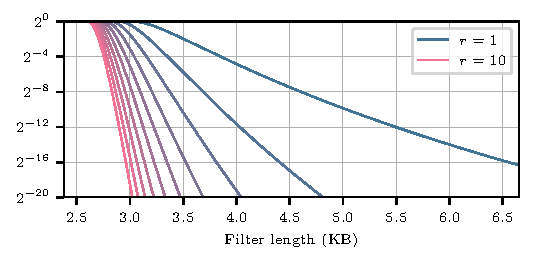
\includegraphics{fig/bf-bound}
  \vspace{-24pt}
  \caption{
    The value of $\zeta_{k,m,n}(q,r)$ (Equation~\ref{eq:zeta}) for $q=2^{64}$,
    $k=16$, $n=100$, varying values of~$r$ (one line per $r$-value) and filter
    length~$m$ (the x-axis).  Note the log-2 scale on the y-axis.
  }
  \label{fig:bf-bound}
\end{figure}

\begin{proof}[Proof of Theorem~\ref{thm:sbf-errep-immutable}]
  \begin{figure*}
\threeColsOneDivideUnbalanced{0.40}{0.27}{0.27}
{
  \vspace{-7pt}
  \experimentv{$\game_{0}(\advB)$}
      \hfill \diffplus{$\game_1$}\\[2pt]
    $M^* \gets \bot$;
    $\salt^* \getsr \bits^\lambda$\\
    $\advB^{\REPO,\QRYO,\HASHO_1}$;
    return $\big[\sum_x \err[x] \geq r\big]$
  \\[6pt]
  \oraclev{$\REPO(\col)$}\\[2pt]
    $M^* \gets \bigvee_{x \in \col} \bmap_m(\HASHO_2(\salt^* \cat x))$;
    $\setS^* \gets \col$;
    return $\langle M^*, Z^* \rangle$
  \\[6pt]
  \oraclev{$\QRYO(\qry_x)$}\\[2pt]
    $X \gets \bmap_m(\HASHO_3(\salt^* \cat x))$;
    $a \gets X = M^* \AND X$\\
    if $\err[x] < \delta(a,\qry_x(\col^*))$ then
          $\err[x] \gets \delta(a,\qry_x(\col^*))$\\
    return $a$
  \\[6pt]
  \oraclev{$\HASHO_c(\salt \cat x)$}\\[2pt]
    $\vv \getsr [m]^k$\\
    if $M^*=\bot$ and $\salt=\salt^*$ and $c=1$ then \com{Caller is~$\advB$}\\
    \tab $\bad_1 \gets 1$; \diffplus{return $\vv$}\\
    if $T[Z,x] = \bot$ then $\vv \gets T[Z,z]$\\
    $T[Z,x] \gets \vv$; return $\vv$
}
{
  \vspace{-2pt}
  \oraclev{$\HASHO_c(\salt \cat x)$}\\[2pt]
    $\vv \getsr [m]^k$\\
    if $M^*=\bot$ and $\salt=\salt^*$ and $c=1$ then\\
    \tab $\bad_1 \gets 1$; return $\vv$\\
    if $T[Z,x] = \bot$ then $\vv \gets T[Z,z]$\\
    $T[Z,x] \gets \vv$\\[2pt]
    \diffplusbox{
    \com{Caller is~$\advB$ or $\QRYO$}\\
    if $c=1$ or $c=3$ then\\
    \tab if $\salt \ne \salt^*$  then return $\vv$\\
    \tab $\Ans[x] \gets \bmap_m(\vv) = M^* \AND \bmap_m(\vv)$\\
    \tab if $\err[x] < \delta(\Ans[x],\qry_x(\col^*))$ then
    \tab\tab $\err[x] \gets \delta(\Ans[x],\qry_x(\col^*))$
    }
    return $\vv$
}
{
  \vspace{-7pt}
  \oraclev{$\QRYO(\qry_x)$}\
      \hfill \diffminus{$\game_1$} \diffplus{$\game_2$}\\[2pt]
    \diffminusbox{%
      $X \gets \bmap_m(\HASHO_3(\salt^* \cat x))$\\
      $a \gets X = M^* \AND X$\\
      if $\err[x] < \delta(a,\qry_x(\col^*))$ then\\
      \tab $\err[x] \gets \delta(a,\qry_x(\col^*))$
    }\\[2pt]
    \diffplusbox{
      $\HASHO_3(Z^* \cat x)$\\
      $a \gets \Ans[x]$
    }
    return $a$
}
\caption{Games 0, 1, and 2 for proof of Theorem~\ref{thm:sbf-errep-immutable}.}
\label{fig:sbf-errep-immutable/games}
\end{figure*}

We will use the following lemma for keyless structures, which is proved in appendix~\ref{sec:keyless-proof}. We use $\errep1$ and
$\erreps1$ to denote the public-representation and private-representation
experiments where the adversary makes a single $\REPO$ query. In writing the
advantage for these games we omit the $q_R$ parameter since it is fixed at 1.

\begin{lemma}\label{thm:lemma1}
  For every $q_R, q_T, q_U, q_H, r, t \geq 0$ and keyless structure~$\Gamma$ it
  holds that
  \begin{eqnarray*}
    \begin{aligned}
      \Adv{\errep}_{\Gamma,\delta,r}(t, q_R, q_T, q_U, q_H) &\leq \\
      & q_R \cdot \Adv{\errep1}_{\Gamma,\delta,r}(O(f(t)), q_T, q_U, q_H) \,,
    \end{aligned}
  \end{eqnarray*}
  where $f(t) = t + (q_R-1)\ticks(\Rep,t) + q_T\ticks(\Qry,t) + q_U\ticks(\Up,t)$.
\end{lemma}
%
\noindent
The proof is by a fairly straightforward hybrid argument. Because~$\Gamma$ is
keyless, in the reduction we simulate $q_R-1$ of the calls to $\REPO$ experiment
and use our own oracles for the remaining query. The best we can do with this
strategy is to ``guess'' which representation the \errep\ adversary will use in
its attack, which results in the~$q_R$ factor in the bound.
%
We defer the full details to Appendix~\ref{app:iproof/lemma-keyless}.

Let $\advA$ be an \errep\ adversary making~$1$ query to~$\REPO$, $q_T$ queries
to $\QRYO$, $0$ queries to $\UPO$, and $q_H$ queries to the random
oracle~$\HASHO$.
%
We make the following assumptions, all of which are without loss of generality.
%
First, all of~$\advA$'s $\QRYO$ queries proceed its $\REPO$ query.
%
Second, we assume that $x\not\in\setS$ for all queries $\qry_x$ to $\QRYO$,
where~$\setS$ was the input to~$\advA$'s $\REPO$ query. This is without loss
because Bloom filtersadmit false positives, but not false negatives
%
Third, we we assume that $|\setS| \leq n$; this is without loss because
otherwise~$\REPO$ outputs~$\bot$ and~$\advA$ gets no advantage.

Fourth, we assume that all of~$\advA$'s $\HASHO$ queries are of the form $Z\cat
x$, where $|Z| = \lambda$.

We begin with a game-playing argument~\cite{bellare2006triple}, then obtain the
final bound via applicaition of Lemma~\ref{thm:lemma1}.
%
\cpnote{Here's the proof sketch.}
%
The high-level goal is to rewrite the game so that the probability that one
of~$\advA$'s queries runs up the score is precisely the false positive
probability for Bloom filters in the usual analytical
setting~\cite{kirsch2006less}. In other words, our goal is transistion into a
setting in which the Bloom filter output by~$\REPO$ is independent of the
outcome of~$\advA$'s other queries.

We begin with the game~$\game_0(\advB)$ defined in
Figure~\ref{fig:sbf-errep-immutable/games}. It is similar to the \errep\ experiment when
executed with~$\advA$, $\Pi$, $\delta$, and~$r$. Indeed, it is not difficult to
see that for every~$\advA$ there exists an adversary~$\advB$ such that
\begin{equation}
  \Adv{\errep}_{\Pi,\delta,r}(\advA) \leq \Prob{\game_0(\advB) = 1}
\end{equation}
and~$\advB$ has the same query resources as~$\advA$.
%
Adversary~$\advB$ executes~$\advA$, forwarding~$\advA$'s oracle queries
to its own oracles in the natural way.

Observe that in game~$\game_0$ the salt used for the representation of~$\setS^*$
is generated prior to executing~$\advB$. Game~$\game_1$ is identical
to~$\game_0$ until the flag~$\bad_1$ gets set by oracle~$\HASHO$. This occurs
if~$\advB$ asks $\HASHO_1(\salt^* \cat x)$, where~$\salt^*$ is the salt generated
at the beginning of the game, and it has not yet called $\QRYO$ (i.e.,
$M^*=\bot$).
%
By the Fundamental Lemma of Game Playing~\cite{bellare2006triple} it follows
that
%
\begin{eqnarray}
  \Prob{\game_0(\advB)=1} &\leq&
    \Prob{\game_1(\advB)=1} + \Prob{\game_1(\advB) \sets \bad_1}\\
  &\leq&
    \Prob{\game_1(\advB)=1} + q_H/2^\lambda \,.
\end{eqnarray}
%
Note that in $\game_1$, the value of~$M^*$ is independent of~$\advB$'s
$\HASHO_1$ queries. In particular, the probability that some bit of~$M^*$ is set
is independent of the choices of~$\advB$.

In game $\game_2$ the $\HASHO$ and $\QRYO$ oracles have been rewritten so that
the winning-condition is computed by $\HASHO$ instead of $\QRYO$. The former
oracle maintains a set~$\Ans$ such that $\Ans[x] = \Qry^{\HASHO_3}(M^*, x)$ for
each query $\salt^* \cat x$; on input of $\qry_x$, oracle~$\QRYO$ simply runs
$\HASHO_3(\salt^* \cat x)$ and returns $\Ans[x]$.
%
We are effectively giving the adverseary credit for RO queries that result in
false positives for the representation of~$\setS^*$, but which it does not
explicitly ask of the~$\QRYO$. Clearly, for every~$\advB$ it holds that
%
\begin{equation}
  \Prob{\game_1(\advB)=1} \leq \Prob{\game_2(\advB)=1} \,.
\end{equation}

We now consider $\Prob{\game_2(\advB)=1}$.
%
Let $\setX$ be the set $\{ x \in \bits^* : \Ans[x] \ne \bot \}$ and $\setT = \{x
\in\setX: \Ans[x] = 1\}$, where $\Ans$ is at is defined when~$\advB$ halts. We
will call~$\setX$ the set of attempts and~$\setT$ the set of false positives.
%
Note that $\setX\intersection\setS^*=\emptyset$ by construction, and that
$|\setX| \leq q_H + q_T$.
%
Hence, the probability that~$\game_2(\advB)=1$ is equal to the probability
that~$|\setT| \geq r$.

For each $x\in\setX$, let $T(x)$ denote the event that $x\in\setT$
%
In the random oracle model for~$H$, the set of random random variables $T(x)$
for each $x\in X$ are independently and identically distributed.
%
Hence, the probability that~$\advB$ succeeds is binomially distributed:
%
\begin{equation}
  \Prob{ |\setT| \geq r } =
     \sum_{i=r}^{q} \binom{q}{i}p^i(1-p)^{q-i} \,,
\end{equation}
%
where $q \leq q_H + q_T$ and $p = \Pr[T(x)=1]$. Note that the mean $\mu$ of this
distribution is simply $pq$, so we can apply the Chernoff bound with
$\delta = r(pq)^{-1}-1$

If we define
$\alpha = \frac{r}{pq}$, then as long as $\alpha > 1$ we can apply a standard
Chernoff bound to simplify this to
\begin{equation}
  \Prob{ |\setT| \geq r } <
     \left(\frac{e^{\alpha-1}}{\alpha^\alpha}\right)^{pq} \,.
\end{equation}

Substituting this value back in for $\Prob{\game_2(\advB)=1}$ and applying
Lemma~\ref{thm:lemma1} to move from the single-representation case to the
general case, we get our final bound of
\begin{equation}
  \Adv{\errep}_{\Pi,\delta,r}(\advA) < q_R \cdot \left(\frac{q_H}{2^\lambda} + \left(\frac{e^{\alpha-1}}{\alpha^\alpha}\right)^{pq}\right) \,.
\end{equation}

%
\todo{DC (lead)}{Apply Lemma~\ref{thm:lemma1} and finish the bound.}
\end{proof}


Recall that the attack against mutable salted filters exploited the fact that
the adversary learned the salt as soon as the filter was created, and that from
this it could compute the hash function on its own. Even if the filter is
mutable, we can prevent this attack from working as long as we require that the
filter under attack be kept secret from adversaries. In fact, we can attain the
following \erreps\ bound.

\begin{theorem}[\erreps\ security of salted BFs]\label{thm:sbf-erreps}
  Let $p' = P_{k,m}(n+r)$.
  For all integers $q_R, q_T, q_H, r, t \geq 0$, if
  $r > p'q_T$, then it holds that
  \begin{eqnarray*}
    \begin{aligned}
      \Adv{\erreps}_{\Pi,\delta,r}(t,\,&q_R, q_T, q_U, q_H) \leq \\
          & q_R \cdot \left[
      \frac{q_H}{2^\lambda} +
      \left(\frac{p'q_T}{r}\right)^re^{r-p'q_T}\right]\,,
    \end{aligned}
\end{eqnarray*}
  where $H$ is modeled as a random oracle.
\end{theorem}

The proof follows a similar structure to that of
Theorem~\ref{thm:sbf-errep-immutable}. The primary differences come from arguing
that without a ``lucky'' guess of the salt the adversary cannot use offline hash
queries to find false positives, and from having to show that the adversary's
access to $\UPO$ does not substantially change the security bound that can be
derived. The first of these is straightforward given the private-representation
setting, but the second requires investigating how much of an advantage the
$\UPO$ oracle can give in a pollution attack, and then moving to games where
this advantage is taken into account.

\begin{proof}[Proof of Theorem~\ref{thm:sbf-erreps}]
  \begin{figure*}
\cpnote{It should be clear from this figure which boxed statments are included
  in which games. Without the context of the text, the way someone would read
  this is ``gamke 0 includes all unboxed statements; game 1 includes all unboxed
  statments and all boxed statements; and game 2 includes all unboxed and
  gray-boxed statements.'' Please clarify this figure so that it's clear what
  statments are included in what games.}
\twoColsNoDivide{0.47}
{
  \vspace{-7pt}
  \experimentv{$\game_{0}(\advB)$}\\[2pt]
    $M^* \gets \bot$;
    $\salt^* \getsr \bits^\lambda$\\
    $\advB^{\REPO,\QRYO,\UPO,\HASHO_1}$;
    return $\big[\sum_x \err[x] \geq r\big]$
  \\[6pt]
  \oraclev{$\HASHO_c(\salt \cat x)$}\hfill \diffminus{$\game_1$}\\[2pt]
    $\vv \getsr [m]^k$\\
    if $\salt=\salt^*$ and $c = 1$ then \com{Caller is~$\advB$}\\
    \tab $\bad_1 \gets 1$; \diffminus{return $\vv$}\\
    if $T[Z,x] = \bot$ then $\vv \gets T[Z,z]$\\
    $T[Z,x] \gets \vv$; return $\vv$
}
{
  \oraclev{$\QRYO(\qry_x)$}\hfill \diffplus{$\game_2$}\\[2pt]
    $X \gets \bmap_m(\HASHO_3(\salt^* \cat x))$;
    $a \gets X = M^* \AND X$\\
    if $\err[x] < \delta(a,\qry_x(\col^*))$ then
          $\err[x] \gets \delta(a,\qry_x(\col^*))$\\
    \diffplus{$\UPO(\up_x)$}\\
    return $a$
  \\[6pt]
  \oraclev{$\REPO(\col)$}\\[2pt]
    \cpnote{I believe this is incorrect, since $\Rep$ is now thresholding.}
    $M^* \gets \bigvee_{x \in \col} \bmap_m(\HASHO_2(\salt^* \cat x))$;
    $\setS^* \gets \col$;
    return $\top$
  \\[6pt]
  \oraclev{$\UPO(\up_x)$}\\[2pt]
    if $w(M) > \ell$ then return $\top$\\
    if $\QRYO(\qry_x) = 1$ then $\err[x] \gets 0$\\
    $M^* \gets M^* \vee \bmap_m(\HASHO_2(\salt^* \cat x))$;
    $\setS^* \gets \up_x(\setS)$;
    return $\top$
}
\caption{Games 0, 1, and 2 for proof of Theorem~\ref{thm:sbf-erreps}.}
\label{fig:sbf-erreps/games}
\end{figure*}

This proof follows a similar structure to the previous one.
%
\cpnote{Don't refer to thoerems this way; say
Theorem~\ref{thm:sbf-errep-immutable}. That way this reference isn't dangling if
we restructure the paper.}
%
The primary distinction is that in the final game, unless the adversary `gets
lucky' and guesses the salt, they should only be able to produce errors with
$q_T$ queries, as opposed to both $q_T$ and $q_H$ queries.
%
Just as in the proof of Theorem~\ref{thm:sbf-errep-immutable}, we will assume
the adversary just makes a single call to $\REPO$ and use Lemma~\ref{thm:lemma1}
to complete the bound. Let $\advA$ be an \erreps\ adversary making exactly 1
call to $\REPO$, $q_T$ calls to $\QRYO$, $q_U$ calls to $\UPO$, and $q_H$ calls
to $\HASHO$. Because $\advA$ creates only a single representation, it will
necessarily lose if it calls $\REVO$ on that representation. We may therefore
assume without loss of generality that $\advA$ makes no calls to $\REVO$, and
because of this we omit $\REVO$ from each of the games.
%
\cpnote{Good. Somehwere in the body we'll need to justify why we include~$\REVO$
in the experiment, since at this point the reader has no reason to believe that
$\REVO$ captures something useful.}

In addition to the assumptions of the previous theorem \todo{DC}{Fix ref}, we
assume without loss of generality that the adversary never uses $\UPO$ to insert
an element into $\col$ which is already present in the set \todo{DC}{Double
check this assumption isn't made above}, and never uses $\UPO$ to insert an
element $x$ where $\QRYO(\qry_x)$ has already been called and has returned a
positive result. Since these insertions do not change the filter and in the
latter case may actually reduce the error count \cpnote{WHAT?? I don't think
that's true. Remember that the error function is \textbf{fixed} at this point.},
the adversary would gain no advantage from performing these updates.
Furthermore, we assume without loss of generality that an adversary halts as
soon as it determines it has accumulated enough errors to win the experiment.

We begin with a game~$\game_0(\advB)$
(Figure~\ref{fig:sbf-errep-immutable/games}) similar to the previous
proof\todo{DC}{fix ref}, except that it also defines an~$\UPO$ oracle. Again, we
observe that for every~$\advA$ there exists a~$\advB$  such that
\begin{equation}
  \Adv{\errep}_{\Pi,\delta,r}(\advA) \leq \Prob{\game_0(\advB) = 1}
\end{equation}
and~$\advB$ has the same query resources as~$\advA$.

Since we are seeking a stronger bound, we now wish to isolate the possibility
that the adversary \emph{ever} guesses the salt, as opposed to just guessing the
salt before calling $\REPO$. This is no longer a trivial task for the adversary
because the representations are private, and so $\REPO$ does not directly reveal
the salt. We therefore set the~$\bad_1$ flag whenever the adversary manages to
guess the salt, without the requirement that $M^* = \bot$. However, since the
adversary is still limited to a total of $q_H$ $\HASHO$ queries, regardless of
when the queries are made, we can follow nearly the same argument as in the
previous proof to get the bound
%
\begin{eqnarray}
  \Prob{\game_0(\advB)=1} &\leq&
    \Prob{\game_1(\advB)=1} + \Prob{\game_1(\advB) \sets \bad_1}\\
  &\leq&
    \Prob{\game_1(\advB)=1} + q_H/2^\lambda \,.
\end{eqnarray}
%
In~$\game_1$, we may now assume that the adversary never guesses the salt in its $\HASHO_1$ queries. This means that none of the inputs to $\HASHO_1$ is ever equal to any input to $\HASHO_2$ or $\HASHO_3$, both of which always use the salt $\salt^*$. Since each $\HASHO$ is modeled as a random oracle, the outputs of $\HASHO_1$ are therefore independent of the outputs of $\HASHO_2$ and $\HASHO_3$.
%
We still cannot move to the binomial distribution for non-adaptive queries,
however, since $\HASHO_2$ and $\HASHO_3$ queries are not necessarily independent
of each other. By one of our starting assumptions, the same input is never
provided twice to $\HASHO_2$ because the adversary never tries to insert an
element which is already in $\col$. We also argue \cpnote{Do you mean assume?} that (without loss of
generality) the same input is never provided twice to $\HASHO_3$, i.e. that the
same element is never queried twice.

\todo{DC}{Replace $\QRYO(x)$ with $\QRYO(\qry_x)$, here and everywhere else.}
On one hand, if a $\QRYO(x)$ call shows that $x$ is already a false positive for
$\pub$, further $\QRYO(x)$ calls cannot increase the adversary's error score. On
the other hand, if a $\QRYO(x)$ call shows that $x$ is not a false positive, it
is still possible for $x$ to become a false positive later on due to $\UPO$
calls. However, the adversary would obtain at least as large a chance of finding
a false positive by calling $\QRYO(y)$ for some previously unqueried $y
\not\in\col$, since the sequence of updates that could make $x$ a false positive
are just as likely to make $y$ a false positive by the independence of
$\HASHO_c$ calls on different inputs. We can therefore assume that the adversary
does not send repeated queries to $\QRYO$.
%
We have now reduced to a case where all hash queries are independent except for
$\QRYO$ and $\UPO$ calls to the same element. By our starting assumptions, an
adversary never calls $\QRYO$ on an element which has already been inserted, so
we need only consider the case of an element being queried before it is
inserted. In fact, doing this can be beneficial to a pollution attack, since
determining with $\QRYO$ that an element is not already a false positive informs
the adversary that inserting that element must necessarily set at least one new
bit in the filter to 1. Since all other possibilities have been eliminated, we
need only consider two types of update the adversary may make:
%
\begin{enumerate}
  \item Inserting an element which is not already in $\col$ and has previously been tested with $\QRYO$, returning a negative result.
  \item Inserting an element which is not already in $\col$ and has not previously been tested with $\QRYO$.
\end{enumerate}
Since calls to $\HASHO_3$ with different choices of $x$ are independent of each
other, and since $\HASHO_3$ uses random sampling, the effects of type 1 updates
on the representation are identically distributed. Similarly, since calls to
$\HASHO_2$ produce independent random results, the effects of type 2 updates on
the representation are also identically distributed. However, the effects of the
two types of update are \emph{not} identically distributed compared to each
other. In particular, making a type 1 update ensures that at least one new bit
in the filter will be set to 1, since the distribution of
$\bmap_m(\HASHO_2(\salt^* \cat x))$ is conditioned on not producing a false
positive. On the other hand, making a type 2 update provides no guarantee about
how many bits in the filter might be set to 1. Type 1 updates are therefore
always preferable for an adversary attempting to produce false positives.

\cpnote{Got here}
In fact, we can make an even stronger statement: it is always optimal for the
adversary to insert $x$ as soon as $\QRYO(x)$ reveals that $x$ is not a false
positive. Since this is a type 1 update, there is no `better' update which could
benefit the adversary more, so there is no reason for the adversary's next
$\UPO$ call to be anything other than $\UPO(\up_x)$. There is also no reason to
make additional $\QRYO$ calls before calling $\UPO(\up_x)$, since calling
$\UPO(\up_x)$ can only increase the probability that further $\QRYO$ calls
produce an error. We therefore assume without loss of generality that $\advB$
inserts $x$ after $\QRYO(x)$ returns a negative result, provided it still has at
least one $\UPO$ call remaining and this insertion would not increase the size
of the underlying set over the maximum number of $n$ elements.

For~$\game_2(C)$, then, we enforce this behavior, changing $\QRYO(x)$ to automatically insert $x$ into $\col$ after computing the correct response to the query. For any $\advB$ for~$\game_1$ we can construct $C$ for~$\game_2$ that simulates $\advB$ to attain the same advantage, forwarding oracle queries in the natural way except that any call of the form $\UPO(x)$ are ignored if $\QRYO(x)$ has been called previously. Ignoring these $\UPO$ calls does not negatively affect the adversary because in~$\game_2$ the original $\QRYO(x)$ call has already inserted $x$ into the set. Furthermore, the `enhanced' $\QRYO$ available to $C$ does not negatively affect $C$ at any point because inserting additional elements into the filter can only increase the probability that later queries return false positives. Then $C$ wins whenever $\advB$ does, and $\Prob{\game_1(\advB) = 1} \le \Prob{\game_2(C) = 1}$.

However, the parameters of the games played by $C$ and $\advB$ are slightly different. In particular, $\advB$ (and, by extension, $C$) may find up to $r$ false positives before halting. When $\advB$ finds these false positives they are by assumption not ever inserted into $\col$, while in the case of $C$ the $\QRYO$ oracle automatically inserts them into the set as soon as they are found. While inserting a false positive does not affect the filter itself in any way, it does increment the number of elements in the underlying set. Therefore if adversaries $\advB$ in~$\game_1$ are limited to representing a set of size $n$, we restrict adversaries $C$ in~$\game_2$ to representing sets of up to size $n+r$.

In~$\game_2$, $\UPO$ queries are actually superfluous. Since every element queried is automatically inserted into the set and the adversary never inserts an element more than once, $\UPO$ calls are now all of type 2. Since these insertions can only increase the chance of each following $\QRYO$ call being a false positive, it is optimal for the adversary to make all $\UPO$ calls at the beginning of the experiment, and then to make all $\QRYO$ calls. But this means we can assume without loss of generality that the adversary makes no $\UPO$ calls at all, since any elements added through $\UPO$ before any $\QRYO$ calls are made could just as easily have been included in the original call to $\REPO$ without affecting the adversary's advantage.

We now therefore only consider the case of a $\REPO$ call followed by the~$\game_2$ version of $\QRYO$ calls. Let $\setX$ be the set of all queries $\qry_x$ which are sent to $\QRYO$ over the course of the experiment. We necessarily have $|\setX| \le q_T$, and each $\qry_x \in \setX$ has some probability of causing an error. Since $\col^*$ never grows to contain more than $n+r$ elements, the false positive probability for each such $\qry_x$ is bounded above by $p_*$, the false-positive probability of a Bloom filter containing $n+r$ elements. So we have, analagously to the previous theorem,
\begin{equation}
   \Prob{\game_2(\advB)=1} \le
     \sum_{i=r}^{q_T} \binom{q_T}{i}p_*^i(1-p_*)^{q_T-i} \,,
\end{equation}
where $q_T$ replaces $q$ and the larger $p_*$ replaces $p$. Applying the same Chernoff bound reduces this to
\begin{equation}
   \Prob{\game_2(\advB)=1} \le
     e^{r-p_*q_T}\left(\frac{p_*q_T}{r}\right)^r.
\end{equation}

Again we apply Lemma~\ref{thm:lemma1} to get a final bound of
\begin{equation}
  \Adv{\erreps}_{\Pi,\delta,r}(\advA) \leq
    q_R \cdot \left[
      \frac{q_H}{2^\lambda} +
      \left(\frac{p_*q_T}{r}\right)^re^{r-p_*q_T}
    \right] \,.
\end{equation}

\end{proof}

\subsection{Keyed BFs}

Salted BFs are \erreps\ secure in general, and are \errep\ secure in the
immutable setting, but are not \errep\ secure when the adversary has access to
an $\UPO$ oracle. Our argument for the \erreps\ security of
salted Bloom filters is made possible by virtue of the structure under attack
not being revealed to the adversary. While this is realistic in many
applications, it may be desirable for the Bloom filter to be public \emph{and}
updatable.
%
Here we show that building a Bloom filter from a PRF suffices for security in
this setting.
%
Let $F:\keys\by\bits^*\to[m]^k$ be a function, fix
integers~$n,\lambda\geq0$, and let $\Pi = \KBF[F,n,\lambda]$.

\begin{theorem}[\errep\ security of keyed BFs]\label{thm:bf-key-bound}
  Let $p' = P_{k,m}(n+r)$.  For integers $q_R, q_T, q_H, r, t \geq 0$ such that
  $r > p'q_T$, it holds that
  \begin{equation*}
    \begin{aligned}
      \Adv{\errep}_{\Pi,\delta,r}(t,\,&q_R,q_T,q_U,q_H) \leq \\
        \Adv{\prf}_F(t,nq_R+q_T+q_U) & +
      \frac{q_R^2}{2^\lambda} +
      \left(\frac{p'q_Rq_T}{r}\right)^re^{r-p'q_Rq_T} \,.
    \end{aligned}
  \end{equation*}
\end{theorem}

Though the bound is similar, the details of this proof differ from the
previous two. In particular, since we are using a PRF, the initial parts of the
proof deal with the adversary potentially being able to break the PRF and with
the possibility of the salts repeating rather than with the adversary being able
to guess the salt.

\begin{proof}
  \begin{figure*}
\todo{DC}{nit: Here and throughout the rest of paper, change $ct$ to
$\mathit{ct}$. The former looks like $c\cdot t$.}
\twoCols{0.47}
{
  \vspace{-7pt}
  \experimentv{$\game_{0}(\advA)$}\\[2pt]
    $\key \getsr \keys$;
    $ct \gets 0$\\
    $i \getsr \advA^{\REPO,\QRYO,\UPO}$;
    return $\big[\sum_x \err_i[x] \geq r\big]$
  \\[6pt]
  \oraclev{$\PRFO(\salt \cat x)$}\hfill\diffminus{$\game_0$}\diffplus{$\game_1$}\\[2pt]
    \diffminus{$\vv \gets F_K(\salt \cat x)$}\\
    \diffplusbox{$\vv \getsr [m]^k$\\
    if $T[Z,x] = \bot$ then $\vv \gets T[Z,z]$\\
    $T[Z,x] \gets \vv$; return $\vv$}
  \\[6pt]
  \oraclev{$\QRYO(i, \qry_x)$}\\[2pt]
    $X \gets \bmap_m(\PRFO(\salt_i \cat x))$;
    $a \gets X = M_i \AND X$\\
    if $\err_i[x] < \delta(a,\qry_x(\col_i))$ then
          $\err_i[x] \gets \delta(a,\qry_x(\col_i))$\\
    return $a$
  \\[6pt]
  \oraclev{$\REPO(\col)$}\\[2pt]
    $ct \gets ct+1$;
    $\setS_{ct} \gets \col$;
    $\salt_{ct} \getsr \bits^\lambda$;
    $c_{ct} \gets |\col|$\\
    $M_{ct} \gets \bigvee_{x \in \col} \bmap_m(\PRFO(\salt_{ct} \cat x))$;
    return $\langle M_{ct}, \salt_{ct}, c_{ct} \rangle$
  \\[6pt]
  \oraclev{$\UPO(i, \up_x)$}\\[2pt]
    if $w(M) > \ell$ then return $\top$\\
    if $\QRYO(\qry_x) = 1$ then $\err_i[x] \gets 0$\\
    $M_i \gets M_i \vee \bmap_m(\PRFO(\salt_i \cat x))$;
    $\setS_i \gets \up_x(\setS_i)$;
    return $\langle M_i, \salt_i, c_i+1\rangle$
}
{
  \vspace{-7pt}
  \experimentv{$\game_2(\advA)$}\hfill\diffplus{$\game_3$}\\[2pt]
    $\key \getsr \keys$;
    $ct \gets 0$;
    $\setZ \gets \emptyset$\\
    $i \getsr \advA^{\REPO,\QRYO,\UPO}$;
    return $\big[\sum_x \err_i[x] \geq r\big]$
  \\[6pt]
  \oraclev{$\REPO(\col)$}\\[2pt]
    $ct \gets ct+1$;
    $\setS_{ct} \gets \col$;
    $\salt_{ct} \getsr \bits^\lambda \setminus \setZ$;
    $c_{ct} \gets |\col|$\\
    $\setZ \gets \setZ \cup \{\salt_{ct}\}$\\
    $M_{ct} \gets \bigvee_{x \in \col} \bmap_m(\PRFO(\salt_{ct} \cat x))$;
    return $\langle M_{ct}, \salt_{ct}, c_{ct} \rangle$
  \\[6pt]
  \oraclev{$\QRYO(i, \qry_x)$}\\[2pt]
    $X \gets \bmap_m(\PRFO(\salt_i \cat x))$;
    $a \gets X = M_i \AND X$\\
    if $\err_i[x] < \delta(a,\qry_x(\col_i))$ then
          $\err_i[x] \gets \delta(a,\qry_x(\col_i))$\\
    \diffplus{$\UPO(i, \up_x)$;}
    return $a$
  \\[4pt]
  \hrule
  \vspace{2pt}
  \oraclev{$\QRYO(i, \qry_x)$}\hfill\diffminus{$\game_3$}\diffplus{$\game_4$}\\[2pt]
    \diffminusbox{
    $X \gets \bmap_m(\PRFO(\salt_i \cat x))$;
    $a \gets X = M_i \AND X$\\
    if $\err_i[x] < \delta(a,\qry_x(\col_i))$ then
          $\err_i[x] \gets \delta(a,\qry_x(\col_i))$\\
    $\UPO(i, \up_x)$;
    return $a$
    }
    \diffplusbox{
    for $j \in [ct]$ do\\
    $\tab X \gets \bmap_m(\PRFO(\salt_j \cat x))$;
    $a_j \gets X = M_j \AND X$\\
    $\tab$if $\err_j[x] < \delta(a_j,\qry_x(\col_j))$ then
          $\err_j[x] \gets \delta(a_j,\qry_x(\col_j))$\\
    $\tab\UPO(j, \up_x)$\\
    return $a_i$}
}
\caption{Games 0--4 for proof of Theorem~\ref{thm:bf-key-bound}.}
\label{fig:kbf-errep/games}
\end{figure*}

We start with a game~$\game_0$ which is essentially the same as the standard
\errep\ experiment on a Bloom filter, given the assumption (without loss of
generality) that the adversary never attempts to construct a representation for
a set with more than $n$ elements. As with the other proofs, it is easy to see
that for any such \errep\ adversary we can make an adversary $\advA$
for~$\game_0$ with the same resources that achieves the same advantage.

Unlike in the previous two proofs, we cannot use Lemma~\ref{thm:lemma1} because
an adversary cannot simulate the oracles without knowing the private key. We use
an alternate approach to gradually reduce to the standard binomial bound
deriving from the non-adaptive false positive probabilities. The first thing we
want to do is to bound the probability that the adversary can break the PRF.

The number of times the PRF is evaluated on distinct inputs is bounded by the
number of queries available to the adversary. In particular, $\QRYO$ and $\UPO$
each call the PRF once, while $\REPO$ may call the PRF up to $n$ times. If the
adversary runs in $t$ time steps, then, the probability it can distinguish the
PRF from a random function is bounded by $\Adv{\prf}_F(t,nq_R+q_T+q_U)$.
%
In~$\game_1$, we have a game which is identical to~$\game_0$ except that it uses
random sampling in place of the PRF. If $\advA$ cannot distinguish the PRF from
a random function then these games are indistinguishable from the adversary's
perspective, so $\Prob{\game_0(\advA) = 1} \le \Adv{\prf}_F(t,nq_R+q_T+q_U) +
\Prob{\game_1(\advA) = 1}$.
%
\cpnote{In fat, this isn't immediate. You show this by a reduction. You want to
show that for every $\advA$ there exists an adversary~$D$ such that
$\Prob{\game_0(\advA)=1} - \Prob{\game_1(\advA)=1} \leq \Adv{\prf}_F(D)$. You
don't need to be super formal about it, but you do need to say how~$D$
executes~$\advA$ and what outputs.}

Our goal is to argue, in a similar manner as to the previous theorems, that all of the oracle calls are independent. In order to guarantee this we must deal with the possibility of a salt collision between different representations. In~$\game_2(\advA)$ we require that all salts be distinct between representations. By the birthday bound, collisions between randomly-generated salts occur with frequency at most $q_R^2/2^\lambda$, so $\Prob{\game_1(\advA) = 1} \le q_R^2/2^\lambda + \Prob{\game_2(\advA) = 1}$.

With guaranteed-unique salts, the result of each $\REPO$, $\UPO$, and $\QRYO$
call for a given representation is independent of the calls for all other
representations. By an almost identical argument to the one in the proof of
Theorem~\ref{thm:sbf-erreps}, we can reduce from any $\advA$ to an adversary
$\advB$ which follows any $\QRYO$ call that finds a true negative with an
$\UPO$ call to insert that element, and therefore move to~$\game_3(\advB)$,
which as in the Theorem~\ref{thm:sbf-erreps} proof performs an update after each
query is made, with the guarantee that $\Prob{\game_1(\advA) = 1} \le \Prob{\game_2(\advB) = 1}$

Finally, we must deal with the possibility that the adversary chooses which
representations to target with $\UPO$ and $\QRYO$ calls based on the result of
$\REPO$, since some representations may be more full than others. In
game~$\game_4$, we allow the adversary credit if a call to
$\QRYO$ produces an error in any of the representations that have been
constructed. Furthermore, the updates made by $\QRYO$ apply to all
representations that are not already full. Since all $\UPO$ calls are
identically and independently distributed, and having more elements in a filter
cannot decrease the false positive rate, the fact that some representations may
become full more quickly than they otherwise would have can only help the
adversary. Similarly, having $\QRYO$ count errors across all representations
never harms the adversary, and so the adversary's advantage may only increase
when moving to~$\game_4$,
i.e. $\Prob{\game_3(\advB) = 1} \le \Prob{\game_4(\advB) = 1}$.

We are now in a situation where we can apply the standard, non-adaptive error
bound. Let $\setX$ be the set of all queries $\qry_x$ made by the adversary over
the course of the game. As in the previous proof, we have $|\setX| \le q_T$.
However, $\qry_x$ may now cause a false positive in any of the representations.
The probability of causing a false positive in a specific representation is
still given by the non-adaptive false positive probability $p'$ for a Bloom
filter containing $n+r$ elements. Since the representations are independent of
each other, the probability of a false positive occurring in any of up to $q_R$
representations is at most $p'q_R$. We can therefore bound the adversary's
success probability using a binomial distribution, similar to before:
\begin{equation}
   \Prob{\game_4(\advB)=1} \le
     \sum_{i=r}^{q_T} \binom{q_T}{i}(p'q_R)^i(1-p'q_R)^{q_T-i} \,.
\end{equation}

Applying the usual Chernoff bound, we find
\begin{equation}
   \Prob{\game_4(\advB)=1} \le
     e^{r-p'q_Rq_T}\left(\frac{p'q_Rq_T}{r}\right)^r.
\end{equation}

So, substituting this bound back into the earlier advantage inequalities, we find the final bound of
\begin{equation*}
  \begin{aligned}
    \Adv{\errep}_{\Pi,\delta,r}(t, q_R,q_T,q_U,q_H) &\leq \\
      \Adv{\prf}_F(t,nq_R+q_T+q_U) & +
    \frac{q_R^2}{2^\lambda} +
    \left(\frac{p'q_Rq_T}{r}\right)^re^{r-p'q_Rq_T}
  \end{aligned}
\end{equation*}
\end{proof}

The fact that both a key and a salt are used in the $\KBF$ construction is
critical. In particular, without the per-representation randomness given by the
salt, we would not be able to argue that $\UPO$ and $\QRYO$ calls are
independent across representations. On the contrary, seeing the representation
of a singleton set $\{x\}$ would immediately allow the adversary to test whether
$x$ was a member in every other representation that had been constructed, simply
by testing whether every bit set to 1 in the representation of $\{x\}$ was also
set to 1 in other representations. Even in the \erreps\ game, using the $\REVO$
oracle on some representations leaks information about other representations,
and again we cannot use the argument that provides the above bound.

We note that Gerbet \etal~\cite{gerbet2015power} suggest using cryptographic
hash functions as one possibility for constructing secure filters, which is
equivalent in our terminology to using a keyed but unsalted filter. The
distinction is that Gerbet \etal assume that representations are kept private
indefinitely, an assumption similar to that underlying our \erreps\ game but
with the stronger restriction that the adversary has no equivalent of a $\REVO$
oracle. Without this assumption that representations are never leaked to the
adversary, however, we emphasize that merely using a long-term secret key
without a per-representation salt does not guarantee security.

\subsection{$\ell$-threshold BFs}

\begin{figure}
  \twoColsNoDivide{0.22}
  {
    \underline{$\Rep^R_K(\col)$}\\[2pt]
      $\salt \getsr \bits^\lambda$;
      $\pub \gets \langle 0^m, \salt\rangle$\\
      for $x \in \col$ do\\
        $\tab \pub \gets \Up^R_K(\pub,\qry_x)$\\
        $\tab$if $\pub = \bot$ then return $\bot$\\
      return $\pub$
  }
  {
    \underline{$\Qry^R_K(\langle M, \salt \rangle,\qry_x)$}\\[2pt]
      $X \gets \bmap_m(R_K(\salt \cat x))$\\
      return $M \AND X = X$
    \\[6pt]
    \underline{$\Up^R_K(\langle M, \salt \rangle,\qry_x)$}\\[2pt]
      if $\hw(M) > \ell$ then return $\bot$\\
      return $\langle M \vee \bmap_m(R_K(\salt \cat x)), \salt \rangle$
  }
  \caption{A slightly modified structure, $\bloom_\mathrm{ft}[R,\ell,\lambda]$ given by
  $(\Rep^R,\Qry^R,\Up^R)$ which uses the Hamming weight of the filter ($\hw$, as
  defined in Section~\ref{sec:prelims}) to decide if the filter is full.}
  \label{fig:bft-def}
\end{figure}

While the above proofs show security bounds for Bloom filters in certain
settings, the bounds may not be as tight as we would like for applications. The
extra factor of $q_R$ in the error bound, for example, may prevent a filter from
achieving good security in practice. We show that a stronger bound can be
achieved using the tweaked Bloom filter construction $\SBF_\mathrm{ft}$, showing
a better bound in the private-representation setting than we had for $\SBF$.
%
\cpnote{When a reviewer read this they'll think: ``why, then, do I care about
$n$-capped filters if $\ell$-threshold filters perform so much better?''}

%
\begin{theorem}[\errep\ security of thresholded BFs]\label{thm:bf-thr-bound}
Let $p_\ell = ((\ell+k)/m)^k$. For integers $q_R, q_T, q_H, r, t \geq 0$ such
that $r > p_\ell q_T$, it holds that
  \begin{equation*}
    \begin{aligned}
      \Adv{\errep}_{\Pi,\delta,r}(t, q_R,q_T,q_U,q_H) &\leq \\
        & \frac{q_R(q_H+q_R)}{2^\lambda} + e^{r-p_\ell q_T}\left(\frac{p_\ell q_T}{r}\right)^r.
    \end{aligned}
  \end{equation*}
\end{theorem}

The distinction between this proof and the proofs for the standard Bloom filter
construction lies in the fact that pollution attacks cannot set more than
$\ell+k$ bits of the filter to 1, regardless of how the attack is conducted.
We therefore assume that the adversary will always be able to produce such a
maximally full filter, and then use a standard binomial-distribution-based bound
to place a limit on the adversarial advantage even in this worst-case scenario.
%
\cpnote{It sounds like you're claiming that pollution attacks are the best the
adversary can do. If this is the case, then you have to prove this.}

\begin{proof}
  \begin{figure*}
\twoCols{0.47}
{
  \vspace{-7pt}
  \experimentv{$\game_{0}(\advA)$}\hfill\diffminus{$\game_0(\advA)$}\diffplus{$\game_1(\advB)$}\\[2pt]
    $ct \gets 0$;
    $\setZ \gets \emptyset$;
    $\setP \gets \emptyset$\\
    \diffminus{$i \gets \advA^{\REPO,\QRYO,\UPO,\HASHO_1,\REVO}$}\\
    \diffplus{$i \gets \advB^{\REPO,\QRYO,\UPO,\HASHO_1}$}\\
    return $\big[\sum_x \err_i[x] \geq r\big] \wedge i \not\in \setP$
  \\[6pt]
  \oraclev{$\HASHO_c(\salt \cat x)$}\\[2pt]
    $\vv \getsr [m]^k$\\
    if $\salt \in \setZ$ and $c = 1$ then \com{Caller is adversary}\\
    \tab $\bad_1 \gets 1$\\
    if $T[Z,x] = \bot$ then $\vv \gets T[Z,z]$\\
    $T[Z,x] \gets \vv$; return $\vv$
  \\[6pt]
  \oraclev{$\QRYO(i, \qry_x)$}\\[2pt]
    $X \gets \bmap_m(\HASHO_3(\salt_i \cat x))$;
    $a \gets X = M_i \AND X$\\
    if $\err_i[x] < \delta(a,\qry_x(\col_i))$ then
          $\err_i[x] \gets \delta(a,\qry_x(\col_i))$\\
    return $a$
  \\[6pt]
  \oraclev{$\REPO(\col)$}\hfill \diffplus{$\game_1$}\\[2pt]
    $ct \gets ct+1$;
    $M_{ct} \gets 0^m$;
    $\salt_{ct} \gets \bits^\lambda$\diffplus{$\setminus \setZ$}\\
    \diffplus{$\setZ \gets \setZ \cup \{\salt_{ct}\}$;}
    $\setS_{ct} \gets \col$\\
    for $x \in \col$ do\\
    $\tab\UPO(ct, \up_x)$\\
    return $\top$
  \\[6pt]
  \oraclev{$\UPO(i, \up_x)$}\\[2pt]
    if $w(M) > \ell$ then return $\top$\\
    if $\QRYO(\qry_x) = 1$ then $\err_i[x] \gets 0$\\
    $M_i \gets M_i \vee \bmap_m(\HASHO_2(\salt^* \cat x))$;
    $\setS_i \gets \up_x(\setS_i)$
    return $\top$
  \\[6pt]
  \oraclev{$\REVO(i)$}\\[2pt]
    $\setP \gets \setP \cup \{i\}$\\
    return $\langle M_i, \salt_i\rangle$
}
{
  \vspace{-7pt}
  \oraclev{$\HASHO_c(\salt \cat x)$}\hfill\diffplus{$\game_2$}\\[2pt]
    $\vv \getsr [m]^k$\\
    if $\salt \in \setZ$ and $c = 1$ then \com{Caller is adversary}\\
    \tab $\bad_1 \gets 1$; \diffplus{return $\vv$}\\
    if $T[Z,x] = \bot$ then $\vv \gets T[Z,z]$\\
    $T[Z,x] \gets \vv$; return $\vv$

  \vspace{6pt}\hrule\vspace{3pt}

  \oraclev{$\REPO(\col)$}\hfill\diffplus{$\game_3$}\\[2pt]
    $ct \gets ct+1$;
    $M_{ct} \gets 0^m$;
    $\salt_{ct} \gets \bits^\lambda\setminus \setZ$\\
    $\setZ \gets \setZ \cup \{\salt_{ct}\}$;
    $\setS_{ct} \gets \col$\\
    for $x \in \col$ do\\
    $\tab\UPO(ct, \up_x)$\\
    \diffplusbox{while $w(M_{ct}) < \ell+k$ do\\
    $\tab i \getsr [m]$;
    $M_{ct}[i] \gets 1$}
    return $\top$

  \vspace{6pt}\hrule\vspace{3pt}

  \experimentv{$\game_4(D)$}\\[2pt]
    $M \gets 0^m$\\
    while $w(M_{ct}) < \ell+k$ do\\
    $\tab i \getsr [m]$;
    $M_{ct}[i] \gets 1$\\
    $D^{\QRYO}$;
      \cpnote{Where's $D$'s $\HASHO_1$ oracle?}\\
    return $\big[\sum_x \err[x] \geq r\big]$
  \\[6pt]
  \oraclev{$\QRYO(\qry_x)$}\\[2pt]
    $X \gets \bmap_m(\HASHO_3(\salt_i \cat x))$\\
    $a \gets X = M \AND X$\\
    $\err[x] \gets a$\\
    return $a$
}
\caption{Games 0, 1, and 2 for proof of Theorem~\ref{thm:sbf-erreps}.}
\label{fig:sbf-erreps/games}
\end{figure*}

As in previous proofs, we assume without loss of generality that there are no
insertions of or queries for elements of $\col$, and we start with a
game~$\game_0$ that is identical to the \erreps\ game for $\KBF_\mathrm{ft}$.
\cpnote{Where is~$\game_0$? Refer to the figure.}

To avoid the unfortunate $q_R$ factor in the bound, we do not make use of
Lemma~\ref{thm:lemma1} in this proof. Because of that, we must find some other
way to ensure that $\REVO$ is not useful to the adversary. In particular, if
there are unique salts across representations, the $\REPO$, $\QRYO$, and $\UPO$
calls for one representation will be independent of those for other
representations, since the unique salt is passed as part of the input. Therefore
in~$\game_1$ we specify that all salts created will be unique, but deny access
to $\REVO$. By the birthday bound, the probability of salts repeating
in~$\game_0$ is no more than $q_R^2/2^\lambda$. If the representations are
independent, calling $\REVO$ would provide no information about other
representations, and would in fact only weaken the adversary by causing some
possible outputs $i \in [q_R]$ to be automatic losses. So we have
$\Prob{\game_0(\advA) = 1} \le q_R^2/2^\lambda + \Prob{\game_1(\advB) = 1}$,
where $\advB$ is an adversary that performs identically to $\advA$ but is
syntactically distinct because it lacks a $\REVO$ oracle.

Next, we want to ensure that the adversary's $\HASHO_1$ queries are independent
of the $\HASHO_2$ and $\HASHO_3$ queries used for $\REPO$, $\QRYO$, and $\UPO$.
Since the $\HASHO_c$ oracles use random sampling to fill a shared table, this
occurs if and only if the adversary calls
$\HASHO_1(\langle\salt_i,x\rangle)$\todo{DC}{Fix syntax}
for some salt $\salt_i$ used by one of the representations created by $\REPO$.
By an argument very similar to that in the previous proofs, the adversary has at
most $q_H/2^\lambda$ probability of calling $\HASHO_1$ with the salt used by
some specific representation. However, since there are now $q_R$
representations, each with a distinct salt, there is at most a
$q_Rq_H/2^\lambda$ probability of the adversary correctly guessing a salt.
In~$\game_1(\advB)$, we set the $\bad_1$ flag if the adversary succeeds in
guessing the salt in this manner, but the flag does not affect the game. The
case of~$\game_2(\advB)$ is identical until the $\bad_1$ flag is set, which
occurs only when a salt is guessed, so we have $\Prob{\game_1(\advB) = 1} \le
q_Rq_H/2^\lambda + \Prob{\game_2(\advB) = 1}$.

We may now assume~\cpnote{Actually, this is by \textbf{construction}! In the
revised game, the adversary is never handed the correct salt, and it's never
handed any RO output whose input is preprended by the salt. it's not the
aadversary never ``guesses'' it, it's that it doesn't matter if it does! This
the real power game-based proofs. Please revise this, here and elsehwere.} that
the adversary never guesses the salt of any of the
representations, and so the outputs of $\HASHO_1$ are independent of the results
of all calls to $\REPO$, $\QRYO$, and $\UPO$. The next oracle we want to target
is $\UPO$. Now that we have a filter threshold, we want to argue that the
adversary cannot use $\UPO$ to mount an effective pollution attack.
%
\cpnote{You're implicitly assuming that pollution attacks are the best we can
do. Why is this true? It doesn't seem to me like it's true. Maybe it is at this
point in the proof, because we've already dealt with the salt guessing? If
that's the case, we can't call it a ``pollution attack'', since this the
experiment has changed.}
%
In~$\game_3(C)$, the $\REPO$ oracle creates the filter as normal and then
randomly sets bits until filter is full (i.e., its Hamming weight is at least
$\ell$), which is $\ell+k$ (since
updates are not allowed when more than $\ell$ bits are set, and a single update
may set at most $k$ bits to 1). For any $\advB$ in~$\game_2$, we can construct
$C$ for~$\game_3$ that obtains at least as large an advantage by having $C$
simulate $\advB$, forwarding all oracle queries in the natural way except that
$\UPO$ queries are ignored, with $C$ simply returning $\top$ to $\advB$ without
performing any additional computations or oracle calls. (Recall that, in the
\erreps setting, the adversry expects $\top$ to be the output of~$\UPO$.) Since $\advB$ does not
query elements which are already in $\col$, the outputs of $\HASHO_3$ calls are
independent of any prior $\HASHO_2$ calls.
%
The probability of such an output producing a false positive is strictly a
function of the number of bits in the filter which have been set to 1.
%
Since at least as many bits have been set to 1 in~$\game_3$ as in~$\game_2$,
every $\QRYO$ call is at least as likely to produce a false positive. Therefore
$\Prob{\game_2(\advB) = 1} \le \Prob{\game_3(C) = 1}$.

In~$\game_3$ we can assume without loss of generality that the adversary makes
no $\UPO$ calls, since the filter is already full and no additional updates will
be accepted. \cpnote{Why assume this? The adversary can make as many $\UPO$
queries it wants and it won't make a difference. So why stop it? The reason not
to is that, as a general good, it's good to keep your assumptions minimal.} Since each
representation is created using independent $\HASHO_2$ outputs and then filled
in a uniform random manner until $\ell+k$ bits are set to 1, and is never
modified afterwards, the representations
themselves are random bitmaps which are uniformly distributed over the set of
$m$-length bitmaps with $\ell+k$ bits set to 1. This allows us to move
to~$\game_4(D)$, where the adversary is given a single arbitrary bitmap $\pub$
of length $m$ with $\ell+k$ bits set to 1 and makes $\QRYO$ calls exclusively
for $\pub$, winning if it produces $r$ errors for that `representation'. Given
an adversary $C$ for~$\game_3$, we construct a $D$ for~$\game_4$ that simulates
$C$. When $C$ makes a $\REPO$ call, $D$ immediately returns $\top$ to $C$, and
when $C$ makes a $\QRYO(i,\qry_x)$ call, $D$ selects a random
previously-unqueried element $y$ and calls $\QRYO(y)$, returning the result to
$C$. \cpnote{What about~$C$'s $\HASHO_1$ queries?} Since representations are uniformly distributed and $\HASHO_3$ calls are
independent of the $\HASHO_2$ calls used to construct the representation, each
$\QRYO$ call made by $D$ has the same chance of producing a hit as the $\QRYO$
call made by $C$ has of producing a false positive.
%
\cpnote{What about queries $(i,\qry_x)$ and $(j,\qry_x)$? $D$'s response will be
the same for both, but $C$ is expecting independent outputs.}
%
The win conditions differ
only in that $D$ wins by accumulating $r$ positive results, whereas $C$ must
accumulate $r$ false positives within a single representation, and so $D$ wins
if $\advB$\todo{DC}{You mean $C$?} does. Therefore $\Prob{\game_3(C) = 1} \le \Prob{\game_4(D) = 1}$.

However, since $\QRYO$ calls with distinct inputs have independent outputs, each $\QRYO$ call made by $D$ has the same probability of producing a false positive. In particular, the probability of any one of the $k$ outputs of $\HASHO_3$ colliding with a 1 bit is $(\ell+k)/m$, and the probability of all $k$ outputs doing so is then $((\ell+k)/m)^k$. If we let $\setX$ be the set of all inputs made to $\QRYO$, we again have a binomial distribution where $q_T$ queries are made. Letting $p_\ell = ((\ell+k)/m)^k$, we have
\begin{equation}
   \Prob{\game_4(D)=1} \le
     \sum_{i=r}^{q_T} \binom{q_T}{i}p_\ell^i(1-p_\ell)^{q_T-i} \,,
\end{equation}
and we can once more apply a Chernoff bound, as long as $p_\ell q_T < r$, to simplify this to
\begin{equation}
   \Prob{\game_4(D)=1} \le
     e^{r-p_\ell q_T}\left(\frac{p_\ell q_T}{r}\right)^r.
\end{equation}

Substituting this into our earlier inequalities yields the final bound of
\begin{equation}
   \Adv{\erreps}_{\Pi,\delta,r}(\advA) \leq
     \frac{q_R(q_H+q_R)}{2^\lambda} + e^{r-p_\ell q_T}\left(\frac{p_\ell q_T}{r}\right)^r.
\end{equation}

\end{proof}


\subsection{Discussion}
\todo{DC}{At a high level, our suggested mitigation is to use salt and to use a
cryptographically strong hash function, but the exact strategy depends on the
setting. If you aren't going to update the structure, then salting is
sufficient. If you're going to update the structure, then salting is still
efficient as long as the structure is never revealed to attacker (i.e., the
party or parites choosing the inputs). If keeping the structure secret isn't
possible, then you need to also use a secret key. How does this mitigation
strategy compared to the mitigations suggested by Gerbet \etal? In particular,
are our filters smaller, larger, or about the same length as theirs?}

\cpnote{How does the $\ell$-threshold bound compare to that of $n$-capping?}

\section{Counting Filters}
\label{sec:counting}
\label{sec:count}
\begin{figure}
  \twoColsNoDivide{0.22}
  {
    \underline{$\Rep^R_K(\col)$}\\[2pt]
      $\salt \getsr \bits^\lambda$\\
      $\pub \gets \langle \zeroes(m), \salt\rangle$\\
      for $x \in \col$ do \\
        $\tab \pub \gets \Up^R_K(\pub, \up_{x,1})$\\
        $\tab$if $\pub = \bot$ then return $\bot$\\
      return $\pub$
    \\[6pt]
      \underline{$\Qry^R_K(\langle \v.M, \salt\rangle,x)$}\\[2pt]
      $\v.X \gets R_K(\salt \cat x)$\\
      for $i \in \v.X$ do\\
        $\tab$if $\v.M[i] = 0$ then return 0\\
      return 1
  }
  {
    \underline{$\Up^R_K(\langle \v.M, \salt\rangle, \up_{x,b})$}\\[2pt]
      if $c \geq n$ then return $\bot$\\
      $\v.M' \gets \v.M$;
      $\v.X \gets R_K(\salt \cat x)$\\
      for $i$ in $\v.X$ do\\
      $\tab$ $a \gets \v.M'[i]$\\
      $\tab$ if $a = 0 \wedge b < 0$ then return $\bot$\\
      $\tab \v.M'[i] \gets \v.M'[i] + b$\\
      $\v.M \gets \v.M'$\\
      return $\langle \v.M, \salt \rangle$
  }
  \caption{Keyed structure $\countbloom[R,\ell,\lambda]$ given by
  $(\Rep^R,\Qry^R,\Up^R)$ is used to define the $\ell$-thresholded version of a
  counting filter. The parameters are a function $R:
  \keys\by\bits^* \to [m]^k$ and integers $\ell, \lambda \geq0$. A concrete scheme
  is given by a particular choice of parameters. The function $\hw'$, used to
  determine if the filter is full, is defined in Section~\ref{sec:prelims}.}
  \label{fig:cbf-def}
\end{figure}

Counting filters are a modified version of Bloom filters which are designed to,
like a count min-sketch, allow for deletion as well as insertion~\cite{fan2000summary}.
Unlike CMSs,
however, counting filters are designed to handle set membership queries rather
than frequency queries. Despite this, the two structures are closely related in
terms of security properties. We show that \errep\ security is similarly
impossible, but employing $\ell$-thresholding allows for \erreps\ security witha
bound that is close to count min-sketch.

\heading{Error function for frequency queries}
%
Unlike with a Bloom filter or count min-sketch, counting filters must account
for two different types of errors: false positives and false negatives. To be as
general as possible, we define a parametrized error function~$\delta$ for
positive $\delta^+, \delta^- \in \R$ as
\begin{equation}
  \delta(x, y) =
  \begin{cases}
    0 & \text{if}\ x = y \\
    \delta^+ & \text{if}\ x = 1, y = 0 \\
    \delta^- & \text{if}\ x = 0, y = 1
  \end{cases}
\end{equation}
This means that false positives are given a weight of $\delta^+$ while false
negatives are given a weight of $\delta^-$, and correct responses are given a
weight of 0.

\subsection{Insecurity of public counting filters}
Any counting filter construction necessarily fails to satisfy \errep\
correctness for the same reasons as in the case of count min-sketch. In
particular, the adversary can call $\REPO(\emptyset)$ to receive an empty
representation, insert an element $x$, observe which counters are incremented by
this insertion, and then delete $x$. By doing this repeatedly, the adversary can
gain information about which elements overlap with which combinations of other
elements, and can therefore mount the same attack described in
Section~\ref{sec:pub-sketch-bad}.

\subsection{Private Thresholded Counting Filters}

\begin{theorem}\label{thm:counting-erreps}
Fix integers $q_R,q_T,q_U,q_H,q_V, r, t \geq 0$, let $p_\ell = ((\ell+1)/m)^k$,
and let
$r' = \lfloor r/\max(\delta^+,k\delta^-) \rfloor$. For all such
$q_R,q_T,$ $q_U,q_H,q_V,r$, and~$t$, if $r' > p_\ell q_T$ then
  \begin{equation*}
  \begin{aligned}
   \Adv{\erreps}_{\Pi,\delta,r}(O(t),\,&q_R,q_T,q_U,q_H,q_V) \leq\\
     & q_R \cdot \left[\frac{q_H}{2^\lambda} + e^{r'-p_\ell q_T}\left(\frac{p_\ell q_T}{r'}\right)^{r'}\right],
  \end{aligned}
\end{equation*}
where $H$ is modeled as a random oracle.
\end{theorem}
The proof combines details from the proofs of count min-sketch bounds and the
proofs of Bloom filter bounds. In particular, we begin by following an argument
as in the count min-sketch case to limit the advantage the adversary can get
from deleting elements and from re-inserting elements of the original set. There
is a difference in the counting filter case in that \emph{inserting} a known
false positive cannot benefit the adversary, while \emph{deleting} it can. This
is the opposite of the count min-sketch case, but the effect on the bound is
quite similar. In each case we give the adversary additional credit for finding
these false positives while constraining them to not modify false positives they
find. This causes $r'$ to appear in the proof bound rather than $r$ in each
case, but because of the different error functions the definitions of $r'$ are
slightly different.
%
After this step, we observe that a counting filter without
deletion behaves the same as an ordinary Bloom filter in terms of how it
responds to queries. We can therefore borrow the arguments used to establish the
bounds in Theorem~\ref{thm:sbf-erreps-th} to finish the proof.
%
We defer the details of the proof to Appendix~\ref{sec:proof/counting-erreps}.
%\begin{proof}
%  \begin{figure*}
\twoCols{0.47}
{
  \vspace{-7pt}
  \experimentv{$\game_{0}(\advA)$}\hfill\diffplus{$\game_1$}\\[2pt]
    $\v.M^* \gets \bot$;
    $\setS \gets \emptyset$;
    $\salt^* \getsr \bits^\lambda$\\
    $\advB^{\REPO,\QRYO,\UPO,\HASHO_1}$;
    return $\big[\sum_x \err[x] \geq r\big]$
  \\[6pt]
  \oraclev{$\HASHO_c(\salt \cat x)$}\\[2pt]
    $\vv \getsr [m]^k$\\
    if $\salt=\salt^*$ and $c = 1$ then \com{Caller is~$\advB$}\\
    \tab $\bad_1 \gets 1$; \diffplus{return $\vv$}\\
    if $T[Z,x] = \bot$ then $\vv \gets T[Z,x]$\\
    $T[Z,x] \gets \vv$; return $\vv$
  \\[6pt]
  \oraclev{$\QRYO(\qry_x)$}\\[2pt]
    $\v.X \gets \HASHO_3(\salt^* \cat x)$;
    $\setS \gets \setS \cup \{x\}$;
    $a = 1$\\
    for $i$ in $\v.X$ do\\
      $\tab$if $\v.M[i] = 0$ then $a = 0$\\
    if $\err[x] < \delta(a,\qry_x(\col^*))$ then
          $\err[x] \gets \delta(a,\qry_x(\col^*))$\\
    return $a$
  \\[6pt]
  \oraclev{$\REPO(\col)$}\\[2pt]
    $\v.M^* \gets 0^m$\\
    $\setS^* \gets \col$\\
    for $x \in \col$ do\\
      $\tab\UPO(\up_x)$\\
    return $\top$
  \\[6pt]
  \oraclev{$\UPO(\up_{x,b})$}\\[2pt]
    if $w'(\v.M^*) > \ell$ then return $\top$\\
    $\v.X \gets \HASHO_3(\salt^* \cat x)$;
    $\v.M' \gets \v.M^*$\\
    for $i$ in $\v.X$ do\\
      $\tab$ if $\v.M'[i] = 0$ and $b < 0$ then return $\top$\\
      $\tab \v.M'[i] \gets \v.M'[i] + b$\\
    if $b > 0$ and $\QRYO(\qry_x) = 1$ then $\err_i[x] \gets 0$\\
    if $b < 0$ and $\QRYO(\qry_x) = 0$ then $\err_i[x] \gets 0$\\
    $\v.M^* \gets \v.M'$;
    $\setS^* \gets \up_{x,b}(\setS^*)$;
    return $\top$
}
{
  \vspace{-7pt}
  \experimentv{$\game_2(\advA)$}\hfill\diffplus{$\game_2$}\\[2pt]
    $\v.M^* \gets \bot$;
    $\setS \gets \emptyset$;
    \diffplus{$\setR \gets \emptyset$; $r' \gets \lfloor r/\max(\delta^+,k\delta^-)\rfloor$}\\
    $\salt^* \getsr \bits^\lambda$\\
    $\advB^{\REPO,\QRYO,\UPO,\HASHO_1}$;
    return $\big[\sum_x \err[x] \geq r\big]$
  \\[6pt]
  \oraclev{$\QRYO(\qry_x)$}\\[2pt]
    $\v.X \gets \HASHO_3(\salt^* \cat x)$;
    $\setS \gets \setS \cup \{x\}$;
    $a = 1$\\
    for $i$ in $\v.X$ do\\
      $\tab$if $\v.M[i] = 0$ then $a = 0$\\
    if $\err[x] < \delta(a,\qry_x(\col^*))$ then
          $\err[x] \gets \delta(a,\qry_x(\col^*))$\\
    if $\err[x] > 0$ then $\setR \gets \setR \cup \{x\}$\\
    return $a$
  \\[6pt]
  \oraclev{$\UPO(\up_{x,b})$}\\[2pt]
    if $w'(\v.M^*) > \ell$\diffplus{$+r'$} then return $\top$\\
    \diffplus{if $x \in \setR$ and $b < 0$ then return $\top$}\\
    $\v.X \gets \HASHO_3(\salt^* \cat x)$;
    $\v.M' \gets \v.M^*$\\
    for $i$ in $\v.X$ do\\
      $\tab$ if $\v.M'[i] = 0$ and $b < 0$ then return $\top$\\
      $\tab \v.M'[i] \gets \v.M'[i] + b$\\
    if $b > 0$ and $\QRYO(\qry_x) = 1$ then $\err_i[x] \gets 0$\\
    if $b < 0$ and $\QRYO(\qry_x) = 0$ then $\err_i[x] \gets 0$\\
    $\v.M^* \gets \v.M'$;
    $\setS^* \gets \up_{x,b}(\setS^*)$;
    return $\top$
  \vspace{6pt}\hrule\vspace{3pt}
  \oraclev{$\UPO(\up_{x,b})$}\hfill\diffminus{$\game_2$}\diffplus{$\game_3$}\\[2pt]
    if $w'(\v.M^*) > \ell+r'$ then return $\top$\\
    if $x \in \setR$ and $b < 0$ then return $\top$\\
    $\v.X \gets \HASHO_3(\salt^* \cat x)$;
    $\v.M' \gets \v.M^*$\\
    for $i$ in $\v.X$ do\\
      $\tab$ if $\v.M'[i] = 0$ and $b < 0$ then return $\top$\\
      \diffminus{$\tab \v.M'[i] \gets \v.M'[i] + b$}\\
      \diffplus{$\tab \v.M'[i] \gets \min(\v.M'[i] + b, 1)$}\\
    if $b > 0$ and $\QRYO(\qry_x) = 1$ then $\err_i[x] \gets 0$\\
    if $b < 0$ and $\QRYO(\qry_x) = 0$ then $\err_i[x] \gets 0$\\
    $\v.M^* \gets \v.M'$;
    $\setS^* \gets \up_{x,b}(\setS^*)$;
    return $\top$
}
\caption{Games 0--3 for proof of Theorem~\ref{thm:scbf-erreps-th}.}
\label{fig:sbf-erreps/games}
\end{figure*}

As with the proof of Theorem~\ref{thm:sbf-errep-immutable}, we derive a bound in
the \erreps1 case and then use Lemma~\ref{thm:lemma1} to move from \erreps1 to
the more general \erreps case. Because we are in the \erreps1 case, we may
assume without loss of generality that the adversary does not call $\REVO$,
since revealing the only representation automatically prevents the adversary
from winning.

We begin with a game~$\game_0$ which has identical behavior to the \erreps1
experiment for a counting filter. As in the proof of
Theorem~\ref{thm:sbf-errep-immutable}, we have a
$\bad_1$ flag that gets set if the adversary ever calls $\HASHO_1$ with the
actual salt used by the representation. By a very similar argument, we can
move to~$\game_1$, where the behavior is different only when the $\bad_1$ flag
is set, with a bound of
\begin{equation}
  \Prob{\game_0(\advA)=1} \leq
    q_H/2^\lambda + \Prob{\game_1(\advA)=1} \,.
\end{equation}

Unlike in the case of a count min-sketch, it is entirely possible for deletions
to benefit the adversary in this game. In particular, if $x$ is found to be a
false positive, deleting $x$ may cause up to $k$ elements of $\col$ to become
false negatives. We therefore move to a game~$\game_2$ where the adversary gets
credit for either a single false positive or for $k$ false negatives whenever it
finds a false positive, but where the adversary cannot delete any false
positives that it finds. We let $r' = \lfloor r/\max(\delta^+,k\delta^-)\rfloor$
represent the number of false positives the adversary has to find in~$\game_2$
in order to win. In order to prevent the adversary from being penalized by the
filter becoming full too early, we also raise the thresold from $\ell$ to
$\ell+r'$ in~$\game_2$. Now for any $\advA$ for~$\game_1$, we can construct
$\advB$ for~$\game_2$ that simulates $\advA$, keeping track of all query
responses and forwarding all oracle queries in the natural way, except that
calls to delete false positives are ignored. Since $\UPO$ never fails for
$\advB$ due to the increased threshold, and since $\advB$ gets automatic credit
for any false negatives that might have been caused by deleting false positives,
$\advB$ succeeds whenever $\advA$ does, i.e.
$\Prob{\game_1(\advA)=1} \le \Prob{\game_2(\advB) = 1}$.

Since the remaining deletions do not cause errors, we can use the same argument
as in the proof of Theorem~\ref{thm:scms-erreps-th} to reduce from $\advB$ to an
adversary $\advC$ which does not make deletions at all. In~$\game_3$, we further
reduce from a counting filter to a normal Bloom filter by capping each of the
counters in the filter at 1. Since no deletions are performed, a counter
in~$\game_3(\advC)$ is nonzero if and only if the same counter
in~$\game_2(\advC)$ is nonzero. So $\QRYO$ behaves the same in~$\game_3$ as it
did in~$\game_2$, and $\Prob{\game_2(\advC)=1} \le \Prob{\game_3(\advC) = 1}$.

Note that~$\game_3$ is actually simulating an ordinary Bloom filter, since all
`counters' in the filter are restricted to the range $\bits$, there are no
deletions, and any insertions just set the corresponding bits to 1. In fact,
this game is identical to~$\game_2$ in the proof of
Theorem~\ref{thm:sbf-erreps-th} except that the adversary need only accumulate
$r'$ errors instead of $r$ errors and the threshold is $\ell+r'$ instead of
$\ell$. An identical argument allows us to reach the binomial bound of
\begin{equation}
   \Prob{\game_3(\advC)=1} \le
     \sum_{i=r'}^{q_T} \binom{q_T}{i}p_\ell^i(1-p_\ell)^{q_T-i} \,,
\end{equation}
where $p_\ell$ is now defined to be $((\ell+k+r')/m)^k$. Then the standard
Chernoff bound, along with Lemma~\ref{thm:lemma1}, yields the final bound of
\begin{equation}
   \Adv{\erreps}_{\Pi,\delta,r}(\advA) \leq
     q_R \cdot \left[\frac{q_H}{2^\lambda} + e^{r'-p_\ell q_T}\left(\frac{p_\ell q_T}{r'}\right)^{r'}\right]s.
\end{equation}
%\end{proof}

\subsection{Discussion}
The results for counting filters are similar to the results for count-min
sketch, as might be expected given the similarities in terms of both the
supported updates and the structure of the representations themselves (any
count-min sketch can be transformed into a counting filter by adding all the
rows together element-wise.) In particular, we again see that counting filters
which are publicly visible cannot provide good security guarantees. This means
that counting filters intended for a security-sensitive setting should be kept
hidden from potential adversaries. Furthermore, our bound relies on
per-representation random salts and $\ell$-thresholding, so these changes should
also be taken into account when constructing secure counting filters. The size
increase of the filters is comparable to the size increase of count
min-sketches, but is distinct in that it depends on the relative weight of false
positives as opposed to false negatives. False negatives impact the bound more
than false positives due to the scaling factor of $k$ that appears in $r'$,
which indicates that applications seeking to minimize false negatives will
require larger filters than those seeking to minimize false positives. This is
distinctly different than in the non-adaptive setting, where false positives are
much more common in counting filters than false negatives, and therefore much
more relevant in determining the minimum size of the filter.


\section{Count-Min Sketches}
\label{cms}
\begin{figure}
  \twoColsNoDivide{0.22}
  {
    \underline{$\Rep^R_K(\col)$}\\[2pt]
      $\salt \getsr \bits^\lambda$\\
      for $i$ in $[1..k]$ do\\
        $\tab \v.M[i] \gets \zeroes(m)$\\
      $\pub \gets \langle \v.M, \salt\rangle$\\
      for $x \in \col$ do \\
        $\tab \pub \gets \Up^R_K(\pub, \up_{x,1})$\\
        $\tab$if $\pub = \bot$ then return $\bot$\\
      return $\pub$
    \\[6pt]
    \underline{$\Qry^R_K(\langle \v.M, \salt\rangle,\qry_x)$}\\[2pt]
      $\v.X \gets R_K(\salt \cat x)$;
      $a \gets \infty$\\
      for $i$ in $[1..k]$ do\\
      $\tab a \gets \min(a, \v.M[i][\v.X[i]])$\\
      return $a$
  }
  {
    \underline{$\Up^R_K(\langle \v.M, \salt\rangle,\up_{x,b})$}\\[2pt]
      $\mathit{full} \gets \bigvee_{i\in[1..k]} [\hw'(M[i]) > \ell]$\\
      if $\mathit{full}$ then return $\bot$\\
      $\v.M' \gets \v.M$;
      $\v.X \gets R_K(\salt \cat x)$\\
      for $i$ in $[1..k]$ do\\
      $\tab a \gets \v.M'[i][\v.X[i]]$\\
      $\tab$ if $a = 0 \wedge b < 0$ then return $\bot$\\
      $\tab \v.M'[i][\v.X[i]] \gets a + b$\\
      $\v.M \gets \v.M'$;
      return $\langle \v.M, \salt, c+b \rangle$
  }
  \caption{Keyed structure $\sketch[R,\ell,\lambda]$ given by
  $(\Rep^R,\Qry^R,\Up^R)$ is used to define count min-sketch variants.
  The parameters are a function $R: \keys\by\bits^* \to [m]^k$ and integers
  $\ell, \lambda \geq0$. A concrete scheme is given by a particular choice of
  parameters. The function $\hw'$, used to determine if the sketch is full, is
  defined in Section~\ref{sec:prelims}.}
  \label{fig:cms-def}
\end{figure}

The count min-sketch (CMS) data structure is designed to concisely estimate the
number of times a datum has occurred in a data stream. In other words, it is
designed to estimate the frequency of each element of a multiset.  The data
structure is similar to a Bloom filter, but instead of a length-$m$ array of
bits it uses a $k$-by-$m$ array of counters. It is designed to deal with streams
of data in the non-negative turnstile model~\cite{cormode2005improved}, which
means the sketch accomodates both insertions and deletions but does not allow
any entries to have a negative frequency. Our construction
$\sketch[R,\ell,\lambda]$ defined in Figure~\ref{fig:bf-def} involves an
$\ell$-thresholded variation of this structure. As in the case of Bloom filters,
this does not significantly change the operation of the sketch in a
non-adversarial setting, since in general~$\ell$ can be closely approximated
given knowledge of~$n$.
%
\cpnote{This isn't clear. What's~$n$? How do I approximate~$\ell$ given ``knowledge'' of~$n$?}
%
In the presence of an adversary, however, we expect this variation to provide
better security bounds.
%
\cpnote{Better than what? If you had capped instead of thresholded? This section
and the previous one should be readable on their own. If you want to bring up
points you made in the last section, that's totally fine, but you need to point
the reader to where they can read more.}

We will show that, in the \errep\ setting, the count min-sketch structure is
insecure regardless of whether $\ell$-thresholding is used or not, and
regardless of the details of the behavior of the function $R$. On the other
hand, we show that \erreps\ security is achievable even under the assumption
that a salted but unkeyed hash function is used, i.e. $\lambda > 0$ but $\keys =
\{\emptyset\}$.

\heading{Non-adaptive error bound}
%
The CMS is designed to minimize the number of elements whose
frequencies are overestimated, while still allowing for reasonably low memory
usage. For a function $\rho$ and integer $\lambda\ge0$, let
$\sketch[\id^\rho,n,\lambda] = (\Rep^\rho,\Qry^\rho,\Up^\rho)$ as defined
previously. If $\col$ is a multiset containing a total of $n$ elements
(counting duplicates as separate elements), i.e. $\col \in \Func(\bits^*,\N)$ in
our syntax, and $x \in \bits^*$ is any string, possibly but not necessarily a
member of $\col$, we define the error probability for a count-min sketch as
\begin{equation}\label{eq:bf-fp}
  \begin{aligned}
    P_{k,m}(n) =
      \Pr\big[&\rho \getsr \Func(\bits^*,[m]^k);
              \pub \getsr \Rep^\rho(\setS): \\
              &\Qry^\rho(\pub, \qry_x) > \qry_x(\setS)+\frac{en}{m} \given \pub \ne \bot
      \big] \,.
  \end{aligned}
\end{equation}

Informally, $P_{k,m}(n)$ is the probability that some~$x$ is overestimated by a
non-negligible amount in the representation of some $\setS$ containing a total
of $n$ elements, when a random function is used for hashing. Cormode and
Muthukrishnan~\cite{cormode2005improved} show that this probability is bounded
above by $e^{-k}$. CMS does not provide a bound for underestimation of
frequencies, since it is designed for use cases where overestimates are
considered harmful but underestimates are not.

\heading{Error function for frequency queries}

The count min-sketch is designed for settings where overestimation in particular
is undesirable, and so provides tight bounds on the size of overestimates, but
makes no guarantees about underestimates. To make the bounds simpler while
staying conservative in our assumptions, we will use an error function that
counts \emph{any} overestimate as an error, not just overestimates larger than
some lower bound of significance. In particular, we define~$\delta$ as
\begin{equation}
  \delta(x, y) =
  \begin{cases}
    1 & \text{if}\ x > y \\
    0 & \text{otherwise.}
  \end{cases}
\end{equation}

\subsection{Insecurity of public sketches}

Unlike in the Bloom filter case, good security bounds cannot be achieved for a
count-min sketch in the \errep\ setting even if salts and/or private keys are
used. The insecurity is due to the relative power of the $\UPO$ oracle compared
to the case of a Bloom filter. Not only does it allow for deletion as well as
insertion, but since updates are \emph{added} to the representation rather than
being combined with bitwise `or', the adversary gains more information from
seeing updates occur. Because of these differences, the adversary can mount
an attack similar to the target-set coverage attack for a Bloom filter even if a
PRF is used for
hashing. First, the adversary calls $\REPO(\emptyset)$ to get an empty
representation. The adversary can then call $\UPO$ to insert an element into the
set, see exactly what the outputs of each of the hash functions are, and then
call $\UPO$ again to delete the element. By doing this repeatedly, an adversary
can determine the outputs of the PRF for $i$ different inputs using $2i$ calls
to $\UPO$. Once a sufficiently large number of PRF outputs has been determined,
the adversary can construct the test and target set used for the target-set
coverage attack. The adversary then calls $\UPO$ several more times to insert
each element of the test set into the sketch, and then
each element of the target set will be overestimated.

In actual use, this specific attack may not be feasible for the adversary.
However, as long as the sketch is public, the adversary can easily determine the
exact results of inserting or deleting any element just by seeing which counters
are incremented or decremented. For this reason it is not enough that the
function used to perform queries and updates is impossible for the adversary to
simulate, since the adversary can build a lookup table just by watching the
sketch as it is updated. Instead, we must require that the sketch itself is kept
secret from the saversary.

\subsection{Private, $\ell$-thresholded sketches}

Given the success of $\ell$-thresholding in the case of Bloom filters, we
continue using this tweak in the case of count min-sketches. Between
thresholding and the use of a per-representation random salt, we are able to
establish an upper bound on the number of overestimates in a count min-sketch.
However, the bound is not quite as good as in the case of a salted and
thresholded Bloom filter, which is unsurprising given the increased flexibility
of the $\UPO$ oracle (which can perform insertions as well as deletions) and
the greater amount of information returned by the $\QRYO$ oracle (frequencies
rather than binary membership queries).

Formally, we consider the structure given by $\Pi = \sketch[H,\ell,\lambda]$ for
an unkeyed hash function $H: \bits^* \to [m]^k$.

\begin{theorem}[\erreps\ security of thresholded BFs]\label{thm:scms-erreps-th}
Let $p_\ell = ((\ell+1)/m)^k$ and $r' = \lfloor r/(k+1) \rfloor$. For integers $q_R, q_T, q_H, r, t \geq 0$ such
that $r' > p_\ell q_T$, it holds that
  \begin{equation*}
  \begin{aligned}
    \Adv{\errep}_{\Pi,\delta,r}(O(t), q_R,q_T,q_U,q_H,q_V) &\leq \\
     & q_R \cdot \left[\frac{q_H}{2^\lambda} + e^{r'-p_\ell q_T}\left(\frac{p_\ell q_T}{r'}\right)^r\right],
  \end{aligned}
\end{equation*}
where $H$ is modeled as a random oracle.
\end{theorem}

The theorem uses several reductions to gradually whittle away at the flexibility
the adversary has in performing repeated insertions, deletions, and queries to
the same elements. The $r'$ in place of $r$ in the bound comes from the fact
that, if the adversary finds that some $x$ is overestimated, it may be able to
produce as many as $k$ additional overestimates by inserting $x$. We take this
into account by automatically giving the adversary credit for all $k$ additional
overestimates as soon as it discovers the false positive. After taking this into
account, we can reduce to the standard binomial argument in which the adversary
seeks to find $r'$ overestimates by making arbitrary queries.

\begin{proof}
  \ignore{\begin{figure*}
\twoColsNoDivide{0.47}
{
  \vspace{-7pt}
  \experimentv{$\game_{0}(\advB)$}\hfill \diffminus{$\game_1$}\diffplus{$\game_2$}\\[2pt]
    $M^* \gets \bot$;
    $\salt^* \getsr \bits^\lambda$\\
    $\advB^{\REPO,\QRYO,\UPO,\HASHO_1}$;
    return $\big[\sum_x \err[x] \geq r\big]$
  \\[6pt]
  \oraclev{$\HASHO_c(\salt \cat x)$}\\[2pt]
    $\vv \getsr [m]^k$\\
    if $\salt=\salt^*$ and $c = 1$ then \com{Caller is~$\advB$}\\
    \tab $\bad_1 \gets 1$; \diffplus{\diffminus{return $\vv$}}\\
    if $T[Z,x] = \bot$ then $\vv \gets T[Z,z]$\\
    $T[Z,x] \gets \vv$; return $\vv$
}
{
  \oraclev{$\QRYO(\qry_x)$}\\[2pt]
    $X \gets \bmap_m(\HASHO_3(\salt^* \cat x))$;
    $a \gets X = M^* \AND X$\\
    if $\err[x] < \delta(a,\qry_x(\col^*))$ then
          $\err[x] \gets \delta(a,\qry_x(\col^*))$\\
    \diffplus{$\UPO(\up_x)$}\\
    return $a$
  \\[6pt]
  \oraclev{$\REPO(\col)$}\\[2pt]
    $M^* \gets \bigvee_{x \in \col} \bmap_m(\HASHO_2(\salt^* \cat x))$;
    $\setS^* \gets \col$;
    return $\top$
  \\[6pt]
  \oraclev{$\UPO(\up_x)$}\\[2pt]
    if $w(M) > \ell$ then return $\top$\\
    if $\QRYO(\qry_x) = 1$ then $\err[x] \gets 0$\\
    $M^* \gets M^* \vee \bmap_m(\HASHO_2(\salt^* \cat x))$;
    $\setS^* \gets \up_x(\setS)$;
    return $\top$
}
\caption{Games 0, 1, and 2 for proof of Theorem~\ref{thm:sbf-erreps}.}
\label{fig:sbf-erreps/games}
\end{figure*}}

As with the proof of Theorem~\ref{thm:sbf-errep-immutable}, we derive a bound in
the \erreps1 case and then use Lemma~\ref{thm:lemma1} to move from \erreps1 to
the more general \erreps case. Because we are in the \erreps1 case, we may
assume without loss of generality that the adversary does not call $\REVO$,
since revealing the only representation automatically prevents the adversary
from winning.

We begin with a game~$\game_0$ which has identical behavior to the \erreps1
experiment for a salted CMS. As in the proofs of
Theorems~\ref{thm:sbf-errep-immutable} and~\ref{thm:sbf-erreps}, we have a
$\bad_1$ flag that gets set if the adversary ever calls $\HASHO_1$ with the
actual salt used by the representation. By an almost identical argument, we can
move to~$\game_1$, where the behavior is different only when the $\bad_1$ flag
is set, with a bound of
\begin{equation}
  \Prob{\game_0(\advA)=1} \leq
    q_H/2^\lambda + \Prob{\game_1(\advA)=1} \,.
\end{equation}

The key differences between this proof and the Bloom filter proof are the more
complex response space of $\QRYO$ ($\N$ rather than $\bits$) and the possibility
of achieving an error through either overestimation or underestimation of the
actual frequency.

%

It is difficult to bound the probability that, if $\QRYO(\qry_x)$ finds that $x$
is overestimated by 1, the adversary can quickly determine which elements to
re-insert into the sketch in order to increase this error beyond the $n\epsilon$
threshold of `significance'. We therefore move to~$\game_2$, where the adversary
gets credit for any response which overestimates the true value, regardless of
the magnitude of the error. Since this can only increase the probability of a
query producing an error, we have
$\Prob{\game_1(\advA) = 1} \le \Prob{\game_2(\advA) = 1}$.

As a first step in dealing with the $\UPO$ oracle, we want to show that deletion
is never helpful for the adversary. So, for any $\advA$, we construct an
adversary $\advB$ that simulates $\advA$, forwarding all oracle queries in the
natural way, except that it ignores any $\UPO(\up_{x,-1})$ calls, i.e. any
deletions. Because deleting $x$ does not change whether $x$ is overestimated or
not, ignoring deletions does not affect whether later calls of the form
$\QRYO(\qry_x)$ will produce an error. Furthermore, if $y \neq x$, then the
probability of $\QRYO(\qry_y)$ causing an error can only increase if $x$'s
deletion is ignored, since the deletion of $x$ decreases counter values without
decreasing the true frequency of $y$. Therefore
$\Prob{\game_2(\advA) = 1} \le \Prob{\game_2(\advB) = 1}$, and we have reduced
to the case of an adversary whose $\UPO$ calls only consist of insertions.

%%

Next, we move from $\advB$ to an $\advC$ that never inserts an element more than
once. Similarly to the previous step, $\advC$ simulates $\advB$, tracking the
elements of $\col$ and forwarding $\advB$'s oracle queries in
the natural way, except that any $\UPO$ queries to insert an element already
present in $\col$ are ignored. First, inserting $x$ does not
change whether $x$ is overestimated or not, so $\advC$ ignoring the re-insertion
does not affect whether later $\QRYO(\qry_x)$ calls will produce an error. For
$y \neq x$, the fact that $\advB$ makes no deletions is key. The value of the
counters associated with $y$ by the hash functions must be at least equal to the
true frequency of $y$, and $\QRYO(\qry_y)$ will find an overestimate if these
counters are all strictly greater than the true frequency. Since updates are
deterministic, re-inserting $x$ can only increment the same counters that were
incremented by the original insertion of $x$, and so this re-insertion cannot
cause $y$ to become overestimated if it was not already. So all $\QRYO$ calls
are just as likely to produce an error for $\advC$ as they are for $\advB$, and
$\Prob{\game_2(\advB) = 1} = \Prob{\game_2(\advC) = 1}$.

As a third step, we move from~$\game_2$ to a~$\game_3$ where the adversary gains
$k+1$ `points' worth of errors for finding an query which produces an
overestimate, but which prevents the adversary from querying elements of $\col$.
These extra points are necessary because, unlike in the case of a Bloom
filter, inserting an overestimated element $x$ can cause other elements of
$\col$ to become overestimated. In particular, if one of the counters
incremented by the insertion of $x$ is shared with an element of $\col$ that is
not overestimated, that element may become overestimated. However, if that
counter is shared with multiple elements of $\col$, that counter is already an
overestimate for all of the elements associated with it, and so no more than one
overestimate can be caused per counter incremented by the insertion of $x$.
Since inserting $x$ increments $k$ counters, at most $k$ errors can be caused in
this way. For any adversary $\advC$ for~$\game_2$, we can construct $D$
for~$\game_3$ that simulates $\advC$ perfectly except that it ignores any oracle
calls that would insert these elements. Since $D$ already gets credit equal to
the maximum number of errors these insertions could cause in addition to the
credit for the original overestimate, $D$ accumulates at least as many errors as
$\advC$ does, and so $\Prob{\game_2(\advC) = 1} \le \Prob{\game_3(D) = 1}$.

Analagously to the proof of~\ref{thm:sbf-erreps-th}, we now move to a
game~$\game_4$ where $\REPO$ randomly fills the sketch to capacity after
inserting the elements of $\col$, so that each row has $\ell+1$ nonzero
counters. For any $D$ for~$\game_3$ we construct $E$ for~$\game_4$ that
simulates $D$, forwarding $\REPO$, $\QRYO$, and $\HASHO_1$ calls but ignoring
$\UPO$ calls. By a very similar argument, $E$ achieves at least the same
advantage as $D$ by having a maximally full filter as soon as $\REPO$ is called,
and so $\Prob{\game_3(D) = 1} \le \Prob{\game_4{E} = 1}$.

The probability of $E$ winning can now be given by another binomial bound. Since
each row of the sketch is a uniformly random bitmap with $\ell+1$ out of $m$
bits set to 1, the probability of any particular $\QRYO$ call causing a
collision within a single row $i$ is $(\ell+1)/m$, and the probability of a
collision in every row (i.e. an error) is $((\ell+1)/m)^k$. The adversary has a
total of $q_T$ attempts, and wins if it accumulates $\lfloor r/(k+1) \rfloor$
successes. So, letting $p_\ell = ((\ell+1)/m)^k$ and
$r' = \lfloor r/(k+1) \rfloor$, we have
\begin{equation}
   \Prob{\game_4(D)=1} \le
     \sum_{i=r'}^{q_T} \binom{q_T}{i}p_\ell^i(1-p_\ell)^{q_T-i} \,.
\end{equation}
Applying the usual Chernoff bound and applying Lemma~\ref{thm:lemma1} turns this
into the final bound of
\begin{equation}
   \Adv{\erreps}_{\Pi,\delta,r}(\advA) \leq
     q_R \cdot \left[\frac{q_H}{2^\lambda} + e^{r'-p_\ell q_T}\left(\frac{p_\ell q_T}{r'}\right)^r\right].
\end{equation}
\end{proof}

\subsection{Discussion}

Unlike in the Bloom filter case, there is no simple tweak that can be performed
to a count min-sketch to provide good \errep\ security bounds. However, the
bound above shows that in settings where sketches can be assumed secret it is
possible to place bounds on the number of overestimates an adversary can cause.
In particular, we recommend the combination of random per-representation salts
and $\ell$-thresholding in order to mitigate possible attacks in the \erreps\
setting.

The bound we achieve is based on the same binomial bound as in the case of Bloom
filters, but has a notable difference in the form of $r'$ replacing $r$. This
negatively impacts the amount of space the filter must take up in order to
provide low error bounds, but because the scaling factor between $r$ and $r'$ is
only $k+1$, the difference should not be unacceptably extreme given reasonable
parameter choices. We also note that it is possible this bound can be improved
to reduce the impact on sketch size, since the initial factor of $q_R$ does not
have an obvious attack associated with it which would make this bound tight.


%\section{Privacy}
%\label{sec:privacy}
%
The semantic security of the immutable case cannot be easily extended to the mutable case. If the same experiment is used, but with the adversary additionally given access to an $\UPO$ oracle, the adversary can often easily learn the composition of the original set using this oracle. For example, with a standard Bloom filter, the adversary can attempt to insert an element of its choice. The representation will remain the same if and only if that element was already in the filter.

There is also the question of whether there is a natural analog to one-wayness for mutable data structures. Even if the adversary is not allowed to choose the underlying data object and must attempt to guess its contents from its public representation, in the mutable case we must assume the adversary can see the representation change over time as updates occur. We assume there is no way to know in advance which updates will be carried out, and hence no known distribution over $\mathcal{U}$. Therefore, to be cautious, we should let the adversary choose the updates. If the adversary can choose and apply any update it likes, the security notion would of course be impossible to achieve (the adversary will know what elements were added by the updates it chose to make). An alternative is to have the two experiments. In each, the adversary chooses two updates with identical leakage, and the oracle either consistently applies the first (in experiment 0) or consistently applies the second (in experiment 1). But this again leads to problems where the adversary can observe whether the representation has changed in order to determine which elements have previously been added to it.

In short, it is extremely unclear how to extend privacy notions to the mutable case without making the adversary so powerful that they can easily discern the contents of the data structures in question.



%%
%% The next two lines define the bibliography style to be used, and
%% the bibliography file.
\bibliographystyle{ACM-Reference-Format}
\bibliography{struct-sec}

\newpage
\appendix

\section{A generic \erreps1 attack against basic Bloom filters}
\label{app:unsalted-attack}
\todo{CP}{Decide whether we want to include the simualtion code. Given how
simple the attack is, I think we can get away with not including it.}

Fix inetgers $\ell, n, \lambda \geq0$, let $H:\bits^*\to[m]^k$ be a function,  and let
$\Pi = \BF[H,t,\lambda]$ as specified in Figure~\ref{fig:bf-def}.
%
The possibility of pre-computing the structure in the \errep1 games yields the
following attack. Given a set $\setT\subseteq\bits^*$ of target queries, the
adversary searches for a set $\setS\subseteq\bits^*$ such that
$\Qry^H(\Rep^H(\setS), x) = 1$ for all $x \in \setT$. We call such a set a
\emph{cover} set.
%
Once a suitable~$\setT$ is found, the adversary queries $\REPO(\setS)$ followed
by $\QRYO(x)$ for each $x\in\setT$.
%
Assuming $|\setT| \geq r$, where~$r$ is the error capacity, the attack succeeds
with probability~$1$.
%
In this appendix we describe a strategy for finding a covering set and evalute
its performance in terms of success rate and computational cost. We will
(conservatively) model~$H$ as a random oracle.

Fix a set of~$s$ \emph{test queries}. Our goal is to find a set~$\col$ of at
most~$n \leq s$ test queries that covers~$\setT$.
%
For each test query~$x$, we ompute $X = \bmap_m(\HASHO(x))$. If we have the the
resources to compute $X_1 \OR \cdots \OR X_n$ for each of the ${s}\choose{n}$
size-$n$ subsets of targets, twe will eventually find a suitable covering set if
such a set exists.
%
The query complexity of this appraoch is modest; we need to make $s+r$ queries
to~$\HASHO$ ($s$ for the test set, $r$ for the target set), one query
to~$\REPO$, and~$r$ queries to~$\QRYO$. However, checking $\binom{s}{n}$ sets
would be infeasible, even for modest choices of $k$, $m$, and $n$. Observe,
hwoever, that there is a lot of sub-structure to exploit in the search.
%
In the remainder, we describe a \emph{heuristic} strategy for finding a
satisfying set (if it exists) in which we need only check about $O(kr)$ sets on
average.

Let $\setT = \{x_1, \ldots, x_s\}$ be the set of test queries, and let $\setR =
\{x_{s+1}, \ldots, x_{s+r}\}$ be the set of target queries.
%
We construct a tree whose vertices are labeled with subsets of~$[s]$ as follows.
%
Let~$\emptyset$ be the root.
%
For each node $I$ and each $w \in [s] \setminus I$, if $\setlen{I} < n$, then let $I
\union \{ w \}$ be a child of~$I$.
%
The new attack works as follows: traverse the tree depth-first, beginning
at~$\emptyset$, until a vertex~$I$ is reached such that each element of $\setR$ is
a false positive for the representation of $\setS_I = \{ x_i : i \in I \}
\subseteq \setT$.
%
Then for every child~$J$ of $I$, the elements of~$\setR$ are false positives
for~$\setS_J$. The adversary may choose any one of these as its query
to~$\REPO$.

The tree has $\binom{s}{n}$ leaves, and it will traverse the entire tree if
there is no solution. Hence, the worst-case runtime is the same as before.
However, we can reduce the search space dramatically in two ways.
%
First, if there is no solution, then often this can be determined without
traversing the tree. Let $M_\setT$ and $M_\setR$ denote the filters
corresponding to the set of test and target queries, respectively.  If for some
$i \in [m]$, the $i$-th bit of $M_\setR$ is set, but the $i$-th bit of $M_\setT$
is not set, then it is immediate that there is no covering set.
%
The second is a greedy heuristic for eliminating branches of the search tree.
The idea is that we only take a branch if it results in covering an additional
bit in~$M_\setR$. More precisely, for each child $J$ of~$I$, we do as follows:
if there is a bit~$i$ such that the $i$-th bit of $M_{\col_J}$ and $M_{\setR}$
are set, but the $i$-th bit of~$M_{\col_I}$ is \emph{not set}, then the
branch~$J$ is taken; otherwise it is not.
%
This optimization results in a heuristic attack, since the search may miss the
optimal solution.

We implemented this attack and evaluated its performance.
Figure~\ref{fig:bf-correct-attk-sim} shows the success rate and average number
of sets checked for a number of simulations and various parameters.
%
Unsurprisingly, the success rate decreases as we increase the number of filter
bits (top-left of Figure~\ref{fig:bf-correct-attk-sim}); however, with $k=4$,
$m=1024$, $n=100$, and $r=1$, a test set of just $512$ elements suffices for a
success rate of nearly $60\%$ (top-right). It is also worth noting that
increasing the error parameter only slightly decreases the success rate
(bottom-left). These results show that even for very pessimistic parameter
choices, the basic Bloom filter is not secure in the \errep1\ sense.
%
Finally, we find that the average number of sets that were tested is about
$O(kr)$ within all of the parameter ranges we tested.

%
\newcommand{\mydot}{{\scriptsize\ding{108}}}
\newcommand{\myex}{{\scriptsize\ding{53}}}
\begin{SCfigure*}
\centering
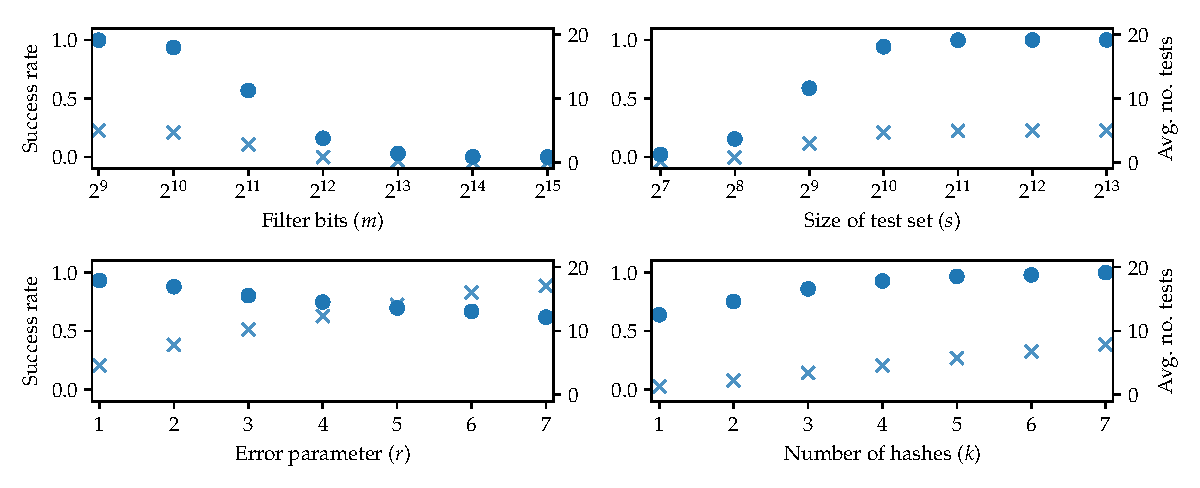
\includegraphics[page=1,scale=0.675]{fig/bf-correct-attk-sim}
\caption{
  %
  Success rate and average-case time complexity for the optimized attack on classic
  Bloom filter.
  %
  Each plot shows the success rate (\mydot), as well as the average number
  of tested sets (\myex), for 1000 executions of
  the attack on simulated inputs.
  %
  Default parameters are $k=4$, $m=2^{10}$, $n=100$, $r=1$, and $s=2^{10}$.
  In each plot, one of these parameters is varied.
}
\label{fig:bf-correct-attk-sim}
\end{SCfigure*}

\ignore{
\heading{Privacy.}
%
\ignore{
  \begin{figure}[t]
    \boxTwoCols{0.48}
    {
      \algorithmv{$\dist[n,\mu]^H$}\\
        $\col \gets \emptyset$;
        for $i\gets 1$ to $n$ do\\
        \tab for $j \gets 1$ to $\mu$ do $\vv_j \gets H(\str(i,j))$\\
        \tab $\col \gets \col \multiunion \{ \str(\vv) \}$\\
        return $\col$
    }
    {
      \adversaryv{$\advA^H$}\\
        for $j \gets 1$ to $\mu$ do $\vv_j \gets H(\str(1,j))$\\
        return $\str(\vv)$\\
    }
    \caption{Distribution~$\dist[n,\mu]$, where $n,\mu \geq0$ are integers, and
    adversary~$\advA$ for attack on ow-rep privacy of~$\BF[k,m,n]$.}
    \label{fig:bf-ow-rep}
  \end{figure}
}
%
The structure~$\BF[k,m,n]$ does not meet our strong notion of \ssrep privacy.
(Indeed, as noted earlier, no keyless data structure can satisfy that
definition.)
%
Even worse, we cannot achieve \owrep privacy for inputs that depend on the
random oracle.
%
Recall that, in the ROM, the distribution~$\dist$ may depend on the random
oracle~$H$.
%
This being the case, we can easily exhibit a distribution with high min-entropy
against which an attacker gets advantage~$1$.
%
Let $\dist$ be a distribution over sets of strings,
parameterized by integers $n,\mu \geq 0$, defined as follows:
%
define a sequence of vectors $\vv_1, \ldots, \vv_n$ so that $\vv_{i}[j] =
H(\str(i,j))$ for each $i\in[n]$ and $j \in [\mu]$.
%
Let $\col = \{\str(\vv_1), \ldots, \str(\vv_n)\}$.
%
Since each query to~$H$ is distinct, the probability that $x \in \col$
for any $x \in \bits^*$ is at most $m^{-\mu}$. Therefore, the point-wise
min-entropy of the distribution is $\mu \cdot \log m$.
%
Now, the attacker can easily compute any $x \in \col$, given access
to~$H$, despite the fact that~$\dist$ has high min-entropy.

Though this attack is theoretical and not particularly interesting in any
practical sense, it is easy to see that \emph{rainbow
tables}~\cite{oechslin2003rainbow}, a practical technique for breaking password
hashes, could be used to deduce the contents.

These negative results for classic BFs in the random oracle model are
reminiscent of the random oracle model \emph{with auxiliary
input}~\cite{unruh2007romaux,dodis2017filling}. In this setting, the adversary
is given a bounded amount of information about the random oracle. This allows us
to model offline computation performed by the adversary before beginning its
attack. Both attacks exploit the fact that the adversary is given the random
oracle \emph{before} choosing its set.
}

\if{0}{
  \heading{Security of RO-independent collections. }
  %
  \cpnote{I vote for cutting this heading entirely. It feels redundant, and the
  restrictions we need to make on the adversary (no stage-1 RO queries) do not
  seem realistic.}
  %
  Both the correctness and privacy attack exploit the fact that the collection may
  depend on the random oracle.
  %
  We remark that, in both settings, security is achievable for collections chosen
  independently of the RO.
  %For correctness, we do not allow the adversary to make
  %queries to~$H$ in its first stage:
  %
  \begin{theorem}[$\BF$ is correct for RO-independent collections]\label{thm:bf-correct*}
    Fix integers $k,m,n,r\ge0$, let $H \colon \bits^* \to [m]$ be a function, modeled as a
    random oracle, and let $\struct_\bloom = \BF[k,m,n]$.
    %
    Let~$\advA$ be an adversary making~$0$ queries to~$H$ in its first stage, and
    $q_{2} \geq 0$ queries to~$H$ and $q_T \geq 0$ queries to~$\QRYO$ in its
    second stage, such that $q_T + q_2 \geq r$.
    %
    Then
    \[
      \Adv{\errep}_{\struct_\bloom,r}(\advA) \leq
      {\dbinom{q_T + q_{2}}{r}} \left( (1-e^{-kn/m})^k + O(1/m) \right)^r\,,
    \]
    \cpnote{We can't use $\Adv{\errep}_{\struct,r}(t,q_T,q_H)$ notation without
    modification.}\tsnote{Added footnote}\cpnote{Muted footnote}
  \end{theorem}
  %
  To be clear, all of the adversary's RO queries are made in its second
  stage.
  %
  The bound reflects the probability that exactly~$r$ of the adversary's stage-2
  queries are a false positive for the set's representation.
  %
  The proof is technically similar to Theorem~\ref{thm:bf-salt-correct}, and so we
  omit the details.
  %

  For privacy, we must restrict the distribution from making any RO queries.  The
  proof is technically similar to Theorem~\ref{thm:bf-salt-ow-rep}, so we again
  omit the details.

  \begin{theorem}[$\BF$ is ow-rep for RO-independent collections]\label{thm:bf-ow-rep*}
    Fix $k,m,n\geq 0$, let $H \colon \bits^* \to [m]$ be a function,
    and let $\struct_\bloom = \BF[k,m,n]$.
    %
    Then for any $t,q_2,\mu \geq 0$, it holds that
    \[
      \Adv{\owrep}_{\struct_\bloom,\mu}(t,0,q_2) \leq
        \frac{(q_2+1)n}{2^\mu} \,,
    \]
    where~$H$ is modeled as a random oracle.
  \end{theorem}
%
}\fi


%\begin{thebibliography}{9}
%\bibitem{bloomfilter} 
%Burton Bloom.
%\textit{Space/time trade-offs in hash coding with allowable errors.}
%Commun. ACM 13, 7 (July 1970), 422-426.
%\end{thebibliography}

%\section{Old-stuff}
%\section{Tom's old Mutuable Hash-Based Filters}
Here we extend the basic Bloom filter syntax to allow for variations on the traditional Bloom filter, e.g. counting Bloom filters~\cite{xxx}, spectral Bloom filters~\cite{xxx}, count-min sketches~\cite{xxx}, stable Bloom filters~\cite{xxx}, etc.   Before giving it, let us briefly describe what is formalized.  Our syntax captures settings in which there is some (potentially empty) initial set~$S$, whose representation~$M$ may undergo updates over time.  Effectively, this allows for expansion of~$S$ to a larger set, or even a multiset, as new elements ``arrive''.    The update algorithm is responsible for altering the current representation.  We allow it to take in a string that encodes inputs needed to carry out the updating.  For example, counting Bloom filters may receive update strings that encode $(x,c)$ where $x \in U$ is the element whose representation should be incremented, and $c \in \mathbb{N}$ is the amount of the increment.  Network applications, such as looking for heavy-hitters across TCP/IP streams seen by a router, may have $x = (\mathrm{IP_{src}},\mathrm{IP_{dst}})$, the source and destintation address of a packet, and~$c$ the number of bytes in the packet payload.  When necessary we will specify what is encoded in the update string, but will assume some implicit and fixed encoding scheme.  Note that our syntax allows for randomized updating.  This accommodates stable Bloom filters, for example, which has a randomized ``forgetting'' feature as part of its update.

\heading{Preliminaries.}
When~$U$ is a set, we let $\multiset{U}{}$ denote the set of all finite multisets of~$U$.  We can denote any multiset~$S$ as $\{(x,\ell) \,|\, x \in U, \ell > 0\}$ where each~$x$ appears exactly once, and each~$\ell$ is an integer.  We define the multiplicity of~$x$ as $\mu_S(x) = \ell$.  We write $|S|= \sum_{(x,\ell)\in S}\mu_S(x)$, and let $\multiset{U}{n}$ denote the set of multisets~$S$ where $|S|=n$.   The notation $S \uplus \{x\}$ denotes multiset union.

\heading{Syntax. }
Fix nonempty sets $U,\Sigma$ and integers $k,m_1,m_2,n>0$ with $m_1 \leq m_2$.  Fix a symbol $\bot \not\in U$.  An $(n,k,[m_1,m_2])$-filter (over universe~$U$) is a tuple  $B=(\Hash,\Init,\Qry,\Update, \Test)$.   
%
The randomized \emph{hash-sampling} algorithm~$\Hash$ samples a size~$k$ family of functions~$\mathcal{H}=\{h_1,h_2,\ldots,h_k\}$ where each $h_i \in  \mathrm{Func}(U,\{0,1,\ldots,m_2-1\})$.  We write $\mathcal{H} \getsr \Hash$ for this operation. 
%
The randomized \emph{initial-representation} algorithm $\Init\colon \multiset{U}{n} \rightarrow \left(\bigcup_{m=m_1}^{m_2}\Sigma^m\right) \times \bits^*$ takes a multiset~$S$ of size~$n$ as input, and outputs representation~$M$ of length~$m_1 \leq m \leq m_2$, and side-information~$\tau$.
%
The determinisitc query algorithm $\Qry\colon \left(\bigcup_{m=m_1}^{m_2}\Sigma^m \right)\times \bits^* \times U \rightarrow \bits^*$ takes a representation $M$, side-information~$\tau$, and an element $x \in U$ as input, and returns a bitstring.  
%
The randomized \emph{update} algorithm $\Update\colon \left(\bigcup_{m=m_1}^{m_2}\Sigma^m \right)\times \bits^* \times \bits^*\rightarrow \left(\bigcup_{m=m_1}^{m_2}\Sigma^m \right) \cup \{\bot\}$ takes a representation~$M$, side-information~$\tau$, and an update string~$\sigma$ as input, and returns an updated representation or the distinguished symbol~$\bot$.  
%
The deterministic \emph{test} algorithm $\Test \colon \multiset{U}{} \times \left(\bigcup_{m=m_1}^{m_2}\Sigma^m \right)\cup\{\bot\} \times \bits^* \times U \rightarrow \bits$ takes a multiset~$S$, a representation~$M$, side-information~$\tau$, and an element~$x \in U$ as input, and returns a bit. \tsnote{The point of $\Test$ is to capture correctness, which is not guaranteed in this setting.  (It isn't something one would actually implement in practice.)  Intuitively, $\Test$ outputs 1 iff $x \in S$ but the representation~$M$ ``says'' it is not.}
%
%We assume that all $\Init,\Qry,\Update,\Test$ all have blackbox access to the functions $h_1,h_2,\ldots,h_k \in \mathcal{H}$, which we denote by writing~$\mathcal{H}$ as a superscript.   

\heading{Correctness. } The kind of filters we capture, here, can have \emph{two-sided} error.  That is, they may result in false-negatives as well as false-positives.  We captures two versions of correctness in Figure~\ref{fig:correctness-mutable}, corresponding to whether or not the adversary is given access to the hash functions used to create and update the multiset representation. \tsnote{These are draft experiments!}

\begin{figure}
\centering
\fpage{.75}{
\hpagess{.6}{.35}
{
\experimentv{$\ExpCorrectSecHash{B}{\distr{U}{n}, A}$}\\
$S \getsr \distr{U}{n}$\\
$ \{h_1,h_2,\ldots,h_k\} \getsr \Hash$\\
$(M,\tau) \getsr \Init^{\HashOracle}(S)$\\
$x \getsr A^{\QryOracle,\UpdateOracle}(S)$\\
if $\Test^{\HashOracle}(S,M,\tau,x) \neq 1$ then\\
\nudge Ret 1\\
Ret 0
}
%
{
\oracle{$\QryOracle(x)$}\\
if $M = \bot$ then Ret $\bot$\\
Ret $\Qry^{\HashOracle}(M,\tau,x)$\\

\medskip
\oracle{$\UpdateOracle(\sigma)$}\\
if $M = \bot$ then Ret $\bot$ \\
$\mathrm{op},\mathrm{val} \gets \sigma$\\
$S \gets S \uplus \{\mathrm{val}\}$\\
$M \getsr \Update^{\HashOracle}(M,\tau,\sigma)$\\

\medskip
\oracle{$\HashOracle(i,x)$}\\
Ret $h_i(x)$\\
}
}
%%%%%%%%%%
\fpage{.75}{
\hpagess{.6}{.35}
{
\experimentv{$\ExpCorrectPubHashBB{B}{\distr{U}{n} , A}$}\\
$S \getsr \distr{U}{n}$\\
$ \{h_1,h_2,\ldots,h_k\} \getsr \Hash$\\
$(M,\tau) \getsr \Init^{\HashOracle}(S)$\\
$x \getsr A^{\QryOracle,\UpdateOracle,\HashOracle}(S)$\\
if $\Test^{\HashOracle}(S,M,\tau,x) \neq 1$ then Ret 1\\
Ret 0
}
%
{
\oracle{$\QryOracle(x)$}\\
if $M = \bot$ then Ret $\bot$\\
Ret $\Qry^{\HashOracle}(M,\tau,x)$\\

\medskip
\oracle{$\UpdateOracle(\sigma)$}\\
if $M = \bot$ then Ret $\bot$ \\
$\mathrm{op},\mathrm{val} \gets \sigma$\\
$S \gets S \uplus \{\mathrm{val}\}$\\
$M \getsr \Update^{\HashOracle}(M,\tau,\sigma)$\\

\medskip
\oracle{$\HashOracle(i,x)$}\\
Ret $h_i(x)$\\
}
}
%%%%%%%%%%%
\fpage{.75}{
\hpagess{.6}{.35}
{
\experimentv{$\ExpCorrectPubHash{B}{\distr{U}{n} , A}$}\\
$S \getsr \distr{U}{n}$\\
$ \{h_1,h_2,\ldots,h_k\} \getsr \Hash$\\
$(M,\tau) \getsr \Init^{\HashOracle}(S)$\\
$x \getsr A^{\QryOracle,\UpdateOracle}(S,\{h_1,h_2,\ldots,h_k\})$\\
if $\Test^{\HashOracle}(S,M,\tau,x) \neq 1$ then Ret 1\\
Ret 0
}
%
{
\oracle{$\QryOracle(x)$}\\
if $M = \bot$ then Ret $\bot$\\
Ret $\Qry^{\HashOracle}(M,\tau,x)$\\

\medskip
\oracle{$\UpdateOracle(\sigma)$}\\
if $M = \bot$ then Ret $\bot$ \\
$\mathrm{op},\mathrm{val} \gets \sigma$\\
$S \gets S \uplus \{\\mathrm{val}\}$\\
$M \getsr \Update^{\HashOracle}(M,\tau,\sigma)$\\

\medskip
\oracle{$\HashOracle(i,x)$}\\
Ret $h_i(x)$\\
}
}
\caption{Trying to define correctness for an $(n,k,[m_1,m_2])$-filter~$B$.  \textcolor{cyan}{Revisit once picture for ``plain'' filters settles.  Also, not exactly right since $\distr{U}{n}$ currently defined to sample from $[U]^n$; here should be multisets.}}
\label{fig:correctness-mutable}
\end{figure}


\heading{Soundness for mutable hash-based filters. } \tsnote{To do.  Same comments as for the simple case, only it's more complicated here because I have no idea what soundness even means in this setting.  Might generically specify two tests as part of the syntax, one for correctness and one for soundness?}


\heading{Privacy of Mutable hash-based filters.} \tsnote{To-do.}


%%%%%%%%%%%%%%%%%%%%%%%%%%%%%%%%%%%%%%%%%%%%%%%%%%%%%%%%%%%%%%%%%
\section{Security Results for Mutable Hash-Based Filters}
\begin{itemize}
\item Prove privacy of ``Stable'' Bloom Filters
\item Ditto for count-min sketch (with and without conservative update)
\item Ditto for scaling BF 
\item Correctness and soundness bounds for these?  (Not sure this is possible without a lot of work; see what's already been done in the papers that propose them)
\end{itemize}

%%%%%%%%%%%%%%%%%%%%%%%%%%%%%%%%%%%%%%%%%%%%%%%%%%%%%%%%%%%%%%%%%

\if{0}
\heading{Multiset-oriented hash-based filters. }
\tsnote{Commented out, but in the source: an alternative way to formalize mutable hash-based filters.  This way directly address the inputs as multisets, instead of starting with a set and then updating the represenation a step at a time.  Not sure which is cleaner and more easily applied to real problems, yet.}

Let $\mathbb{M}_\mathcal{U}$ be the set of multisets over~$\mathcal{U}$.  We can denote any multiset as $\{(x,\ell) \,|\, x \in \mathcal{U}, \ell \in \mathbb{N}\}$, and for a particular multiset~$S$ we define the multiplicity of~$x$ as $\mu_S(x) = \ell$ where $(x,\ell)\in S$.

An $(n,k,[m_1,m_2])$-filter with operations is a tuple  $B=(\Hash,\Rep,\Qry, \mathcal{F})$.  
The set $\mathcal{F}$ is the finite collection of allowable operations.  All operations are of the form 
$f: \mathbb{M}_{\mathcal{U}} \times \mathbb{M}_{\mathcal{U}} \rightarrow \mathbb{M}_{\mathcal{U}} \cup \{\bot\}$.  
%
The deterministic representation algorithm $\Rep\colon \mathbb{M}_\mathcal{U} \rightarrow \bigcup_{m=m_1}^{m_2}\Sigma^m$ takes a multiset~$S$, and outputs representation~$M$ of length~$m_1 \leq m \leq m_2$, or the distinguished symbol~$\bot$.  We assume that if the multiset~$S=\{(x_1,\ell_1),(x_2,\ell_2),\ldots,(x_t,\ell_t)\}$ is such that $n < \sum_{i=1}^t \ell_i$ then $\Rep(S)=\bot$.
%
The randomized hash-sampling algorithm~$\Hash$ is as before.
%
The determinisitic query algorithm $\Qry$... \tsnote{Not sure how to define this!  See my comment, below...}

%Correctness is defined as follows.  Let $S,T$ be arbitrary multisets and let~$f$ be an arbitrary operation in $\mathcal{F}$.  If $f(S,T) = S'\neq \bot$, then for all $x \in S'$ we demand that $\Qry(\Rep(S'),x)=1$.  \tsnote{might need a stronger condition that this holds for any sequence of operations that do not result in $\bot$.}

Let us see how this syntax captures various kinds of Bloom filters.  First, let $\Sigma = \mathbb{N}$ and define $f_{\mathrm{add}}(S,T)=\{(x,\mu_S(x)+\mu_T(x)) \,|\, x \in \mathcal{U}\}$ and $f_\mathrm{del}(S,T) = \{(x,\min\{0,\mu_S(x)-\mu_T(x)\}) \,|\, x \in \mathcal{U} \}$.  Define $\Rep(S')$ as follows: for each $(x,\ell)\in S'$ and $j\in\{1,2,\ldots,k\}$, set $M[h_j(x)]=\ell$.   Finally, define $\Qry(M,x) = 1 \Leftrightarrow \forall j \in \{1,2,\ldots,k\},\; M[h_j(x)] > 0$.  This allows us to capture counting Bloom filters. \tsnote{Does it?  Acutally, you might want $\Qry(M,x)$ to return a number, i.e., a counter value.  How do you define correctness then?}

\tsnote{There are more direct ways to formalize counting Bloom filters, like the syntax above.  But this less direct way will allow us to capture other kinds ``advanced'' Bloom filters proposed in the literature or (more importantly) used in practice. For example, $f_{\mathrm{setify}}(S,T)=\{(x,1) \,|\, x \in \mathcal{U} \mbox{s.t. } \mu_S(x)>0, \mu_T(x)>0\}$.  On the other hand, we may end up deciding it is overkill... }
\fi
